%==============================================================================
\FloatBarrier
% \section{Noise correlations}
% %------------------------------------------------------------------------------
%
% The  \autoref{sec:bg-noisecorr} for an overview of noise correlations.
%
% For the vast majority of neurons
% For contrast-selectivity, the vast majority of neurons do in fact encode stimuli monotonically --- a higher contrast will illicit a stronger neural response. With this in mind, the most beneficial pair-wise neural correlations will nearly always be more negative correlations. This is the direction which more perpendicular to the stimulus encoding direction within the 2-D plane of responses.
%
%
% %% older content
%
% The firing rate of neurons in the sensory system will vary trial-to-trial, even if the stimulus presented is the same.
% The manner in which these responses fluctuate together is known as the noise correlation between neurons.
% If there are positive noise correlations, the changes in neural activity across a population will increase and decrease together.
% Long-standing theoretical work has indicated such correlations will hamper the ability of upstream neurons to accurately decode the stimulus% [cite]
% , which is in keeping with experimental results demonstrating attention reduces noise correlations \citep{Cohen2009}.
% This fits with intuition --- if stimulus A is encoded with one firing rate across a population and stimulus B with a slightly higher rate, a systematic increase or decrease in the population firing rates can easily cause A and B to be confused with one another.
%
% However, recent theoretical results indicate that for a more realistic non-homogeneous population of neurons, neural correlations do not limit the population-wide information as the number of neurons increases \citep{Oram1998,Averbeck2006,Ecker2011}.
%
% Other studies have indicated that noise correlations are beneficial to population encoding, provided that the structure of the correlations means the correlations are orthogonal to the direction in which stimuli are encoded.
% % cite pouget, latham, franke2016
%
% A recent paper by \citet{Gu2011} on neurons recoded from the macaque dorsal \ac{MSTd} before and after training in a head direction discrimination task, found that although pairwise noise correlations between neurons are reduced with training, this does not yield an increase in performance in a decoder.
% We will see if these findings hold here as well.
%
%
% \subsection{Methods}
% \label{sec:dec-meth-noise}
%
% The noise correlation was investigated by considering how strongly correlated the spike counts during test stimulus presentation.
% % (this could have been done using the data from the sample presentation, which would probably have been a better idea).
%
% To evaluate the strength of noise correlations, the Pearson $r$ correlation coefficient was used.
% For two random variables $X$ and $Y$, this is given by
% \begin{equation}
% r(X,Y) = \frac{\operatorname{cov}(X,Y)}{\operatorname{var}(X) \, \operatorname{var}(Y)}
% \end{equation}
% and provides a version of the covariance between the $X$ and $Y$ which is normalised again their standard deviations.
% This means $-1 \le r \le 1$ indicates how well $X$ and $Y$ fit a straight line relationship of either positive or negative slope, regardless of the gradient of the line, which could be changed by rescaling either $X$ or $Y$.
% If $r=\pm1$, there is a perfect linear relationship between $X$ and $Y$, whereas $r=0$ when $X$ and $Y$ are completely independent.
%
% For each individual session, the Pearson $r$ correlation coefficient was computed between the spike counts during test stimulus presentation between pairs of channels, across all the trials in the session.
% $r$ was computed for each pair and each condition, and the mean was taken across all of these.
%
%
% \subsection{Results}
%
% For both \ac{V1} and \ac{V4}, the average noise correlation between pairs of channels seem to remain stable for \ac{M1} and decrease by a small margin for \ac{M2} (see \autoref{fig:noise_r_all}).
% The increase in noise correlation for \ac{M1} \ac{V1} for the last two sessions (session numbers 358 and 359) is due to a decline in data quality and an increase in noise from artificial sources.
% There is a large amount of variance in the noise correlations for different pairs, so the decline in mean correlation for \ac{M2} does not seem very large considering the amount of variance.
%
%
% \begin{figure}[htb]
%     \centering
%     \subfloat[][\label{fig:noise_r_v1_all}\ac{V1}]{
% %         \includegraphics[width=0.47\linewidth]{%
% % ./rcoef_2013-04-09/rcoef_sess_meanpc_2013-04-09/png/rcoef_sess_meanpc_v1_both.png}
% %        \includegraphics[width=0.47\linewidth]{figs/decoding/rcoef_sess_meanpc_v1_both}
%         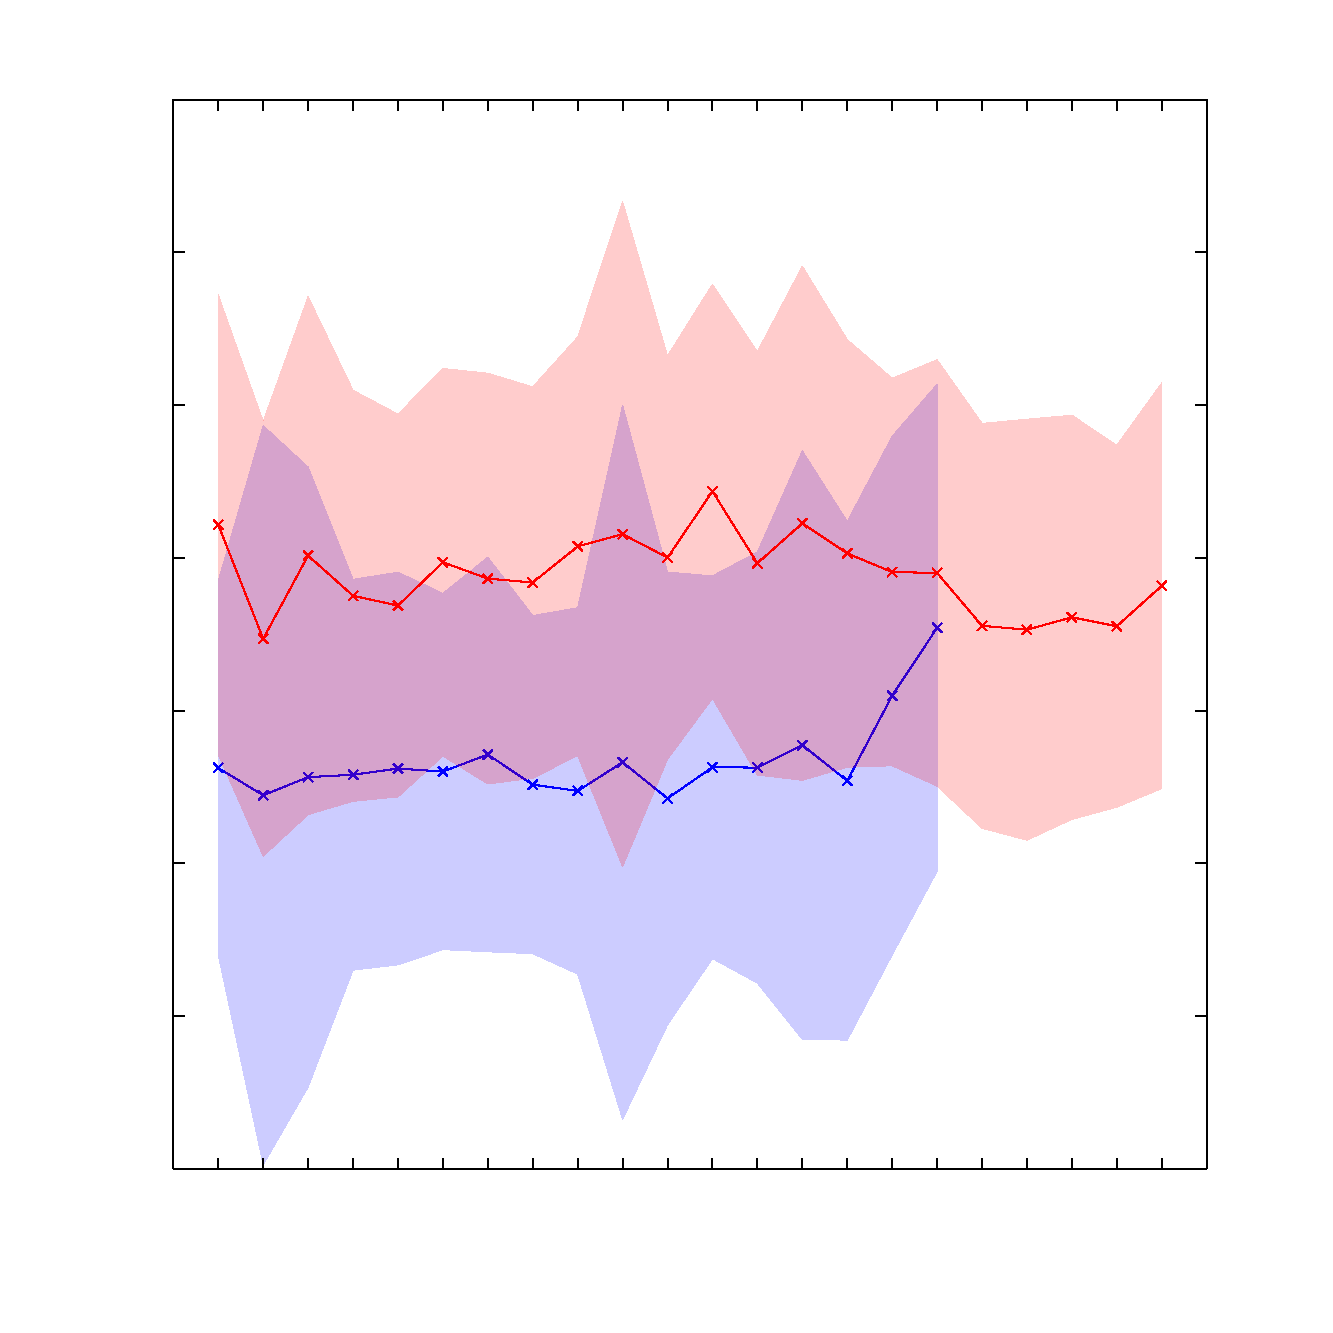
\includegraphics[width=0.47\linewidth]{figs/decoding/rcoef_sess_meanpc_v1_both.pdf}
% }
%     ~~
%     \subfloat[][\label{fig:noise_r_v4_all}\ac{V4}]{
% %         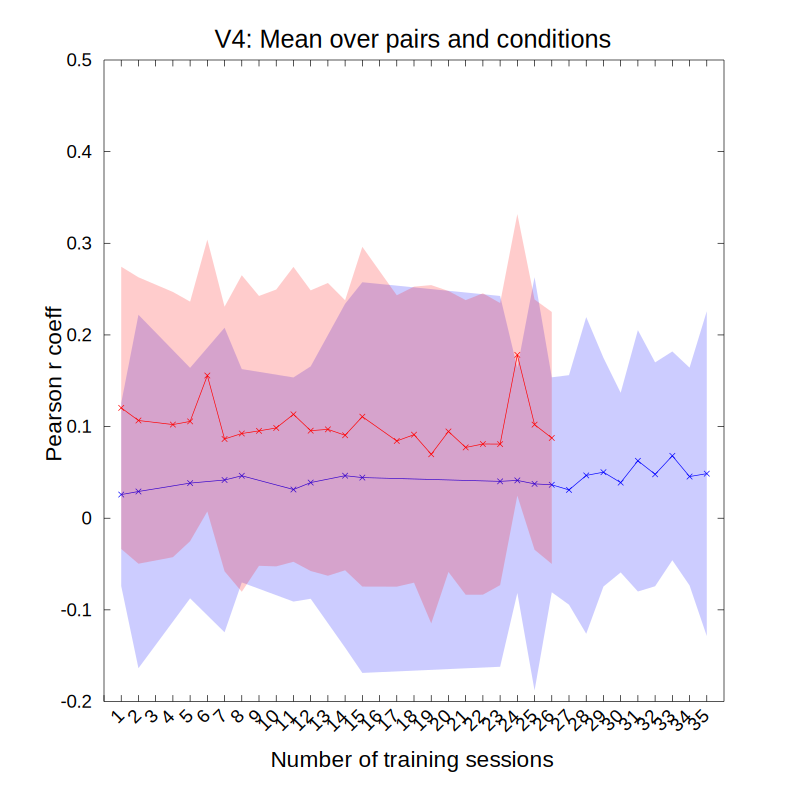
\includegraphics[width=0.47\linewidth]{%
% % ./rcoef_2013-04-09/rcoef_sess_meanpc_2013-04-09/png/rcoef_sess_meanpc_v4_both.png}
%         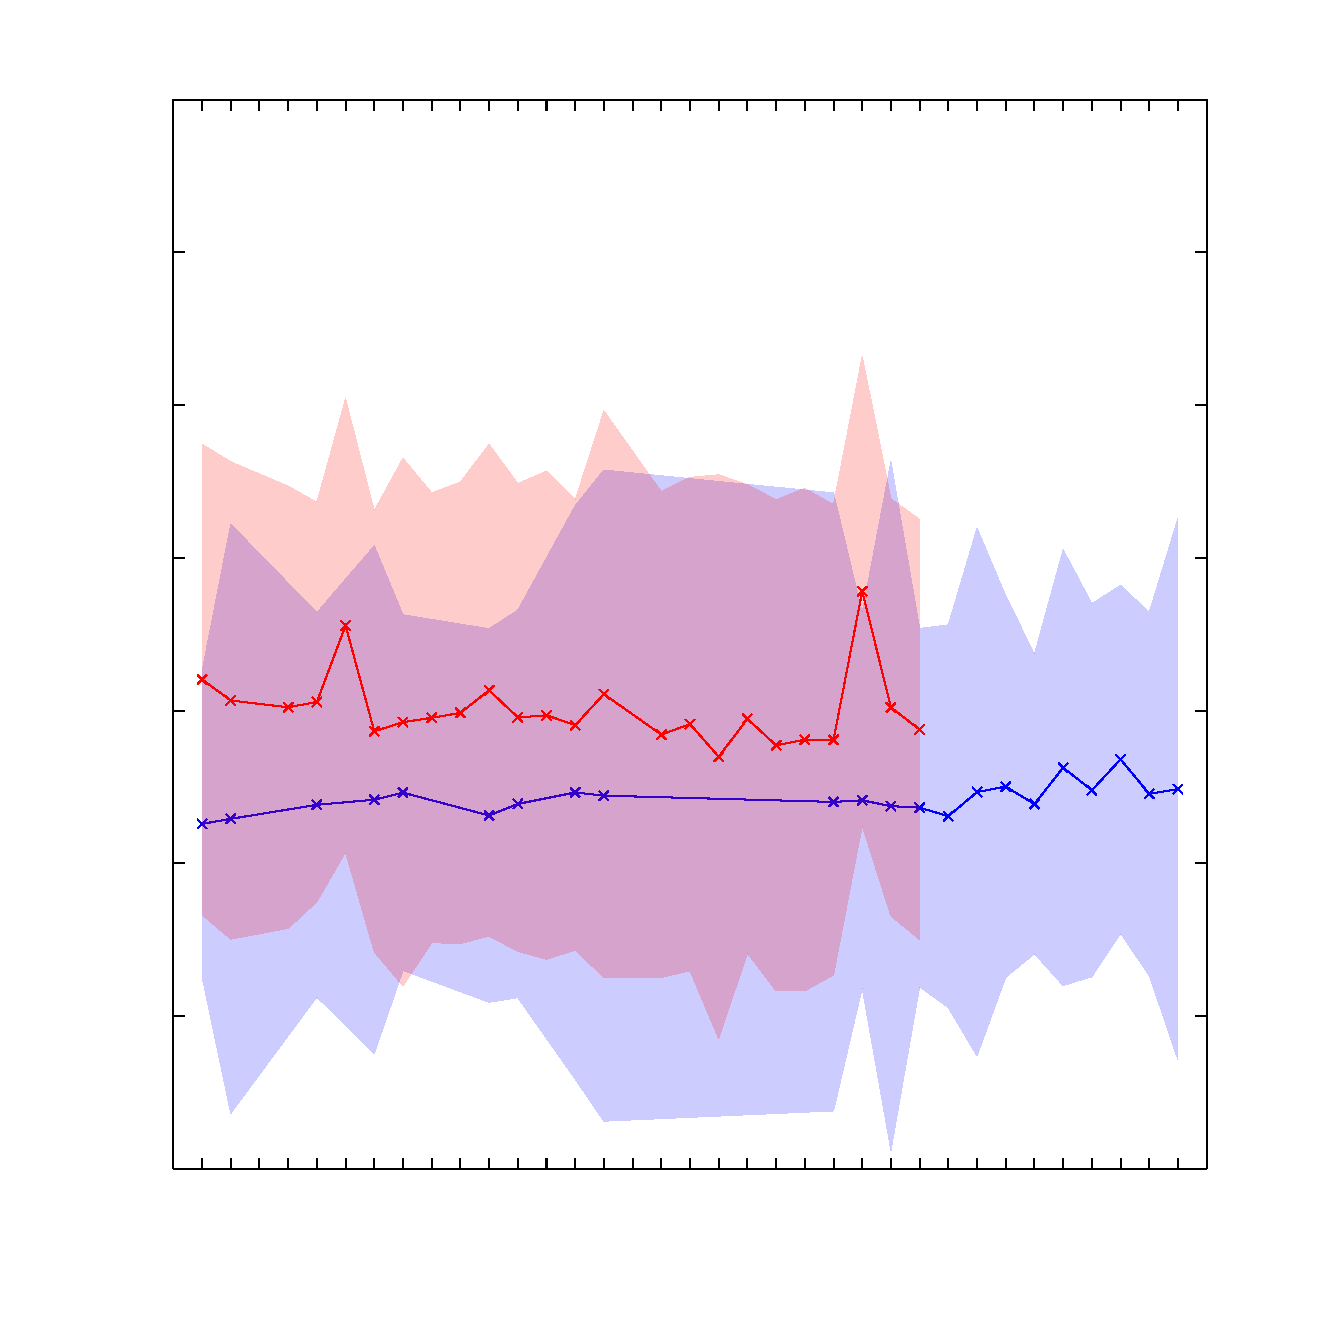
\includegraphics[width=0.47\linewidth]{figs/decoding/rcoef_sess_meanpc_v4_both.pdf}
% }
%     \caption{Change in noise correlations with learning.
% \protect\subref{fig:noise_r_v1_all}:~\ac{V1}.
% \protect\subref{fig:noise_r_v4_all}:~\ac{V4}.
% Blue:~\ac{M1}.
% Red:~\ac{M2}.
% On the x-axis, the number of sessions since the animal began training in the part of the visual field retinotopic to the recording site is shown.
% Line: pearson r coefficient, averaged across the possible pairings between channels for each of the 14 trial conditions.
% Shaded region indicates one standard deviation from mean.
% }
%     \label{fig:noise_r_all}
% \end{figure}
% % \marginnote{In \autoref{fig:noise_r_all} and \autoref{fig:noise_r_hist}, the text is too small due to saving the figure with transparencies in PNG format; if I could get the SVG to load correctly, the text would be sized correctly.}
%
% \autoref{fig:noise_r_hist} is intended to reproduce \citet[Figure 2C]{Gu2011}, with the distribution of $r$ shown across pairs for one pre-training and one post-training session.
% These sessions were chosen from a restricted set of sessions which did not have problems with artificially high correlations from the motion artifact, and selected from this set such that they were as close to the start and end of the training period as possible.
% However, this selection was made before the set of trials was redacted as mentioned in \autoref{sec:dec-meth-noise}, so the sessions selected could possibly be made further apart.
%
% The data presented in \autoref{fig:noise_r_hist} shows that the distribution of noise correlation pairs does not move significantly for \ac{M1} \ac{V1}, which is contrasted by a clear decrease for \ac{M2} \ac{V1}.
% It should be noted though that the distribution for \ac{M2} \ac{V1} begins higher than \ac{M1} and decreases to a similar value as \ac{M1} \ac{V1}.
% For \ac{V4}, there is an increase in mean noise correlation for \ac{M1} and a decrease for \ac{M2}, though as \ac{M2} begins higher than \ac{M1} the two do tend toward to one another.
%
% Cherry-picking is a significant problem here, as there is sizable day-to-day variation in the noise correlation across the pairs.
% Choosing a session where there is more noise correlation than neighbouring sessions at the beginning of training and less at the end of training will give the impression that there is a more significant decrease in noise correlations.
% More effort should be made to counter inadvertently cherry-picking in the session selection, as \autoref{fig:noise_r_j1_pmc} indicates this may be one reason for such a sizable decrease in noise correlation for \ac{M2} \ac{V1}.
%
% \begin{figure}[htbp]
%     \subfloat[][\label{fig:noise_r_b1_hist}]{
%         \centering
% %         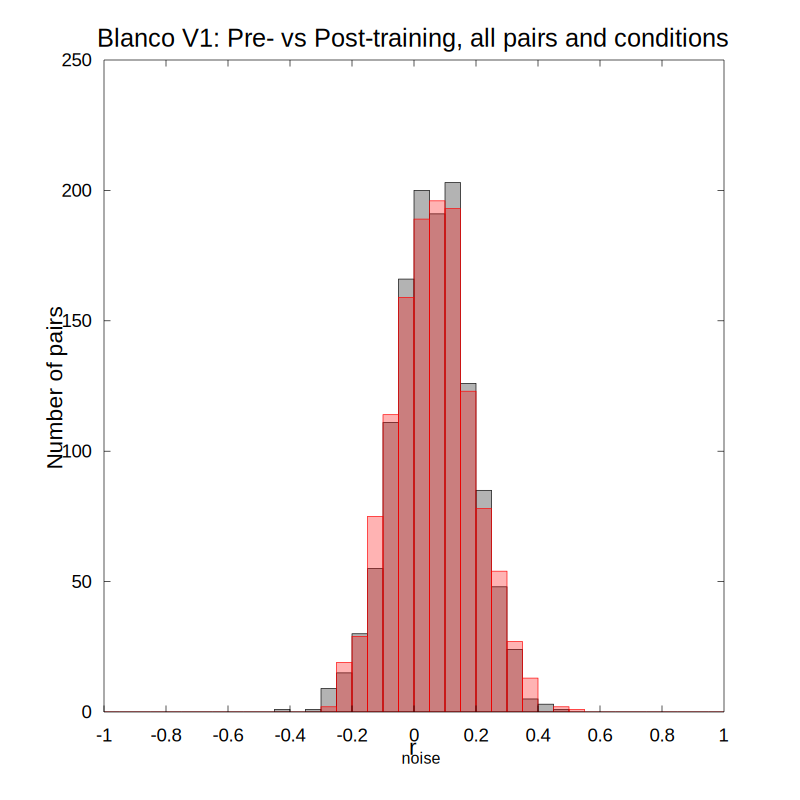
\includegraphics[width=0.47\linewidth]{%
% % ./rcoef_2013-03-25/rcoef_sess_histallover_2013-03-25/png/rcoef_sess_histallover_v1_blanco.png}
%         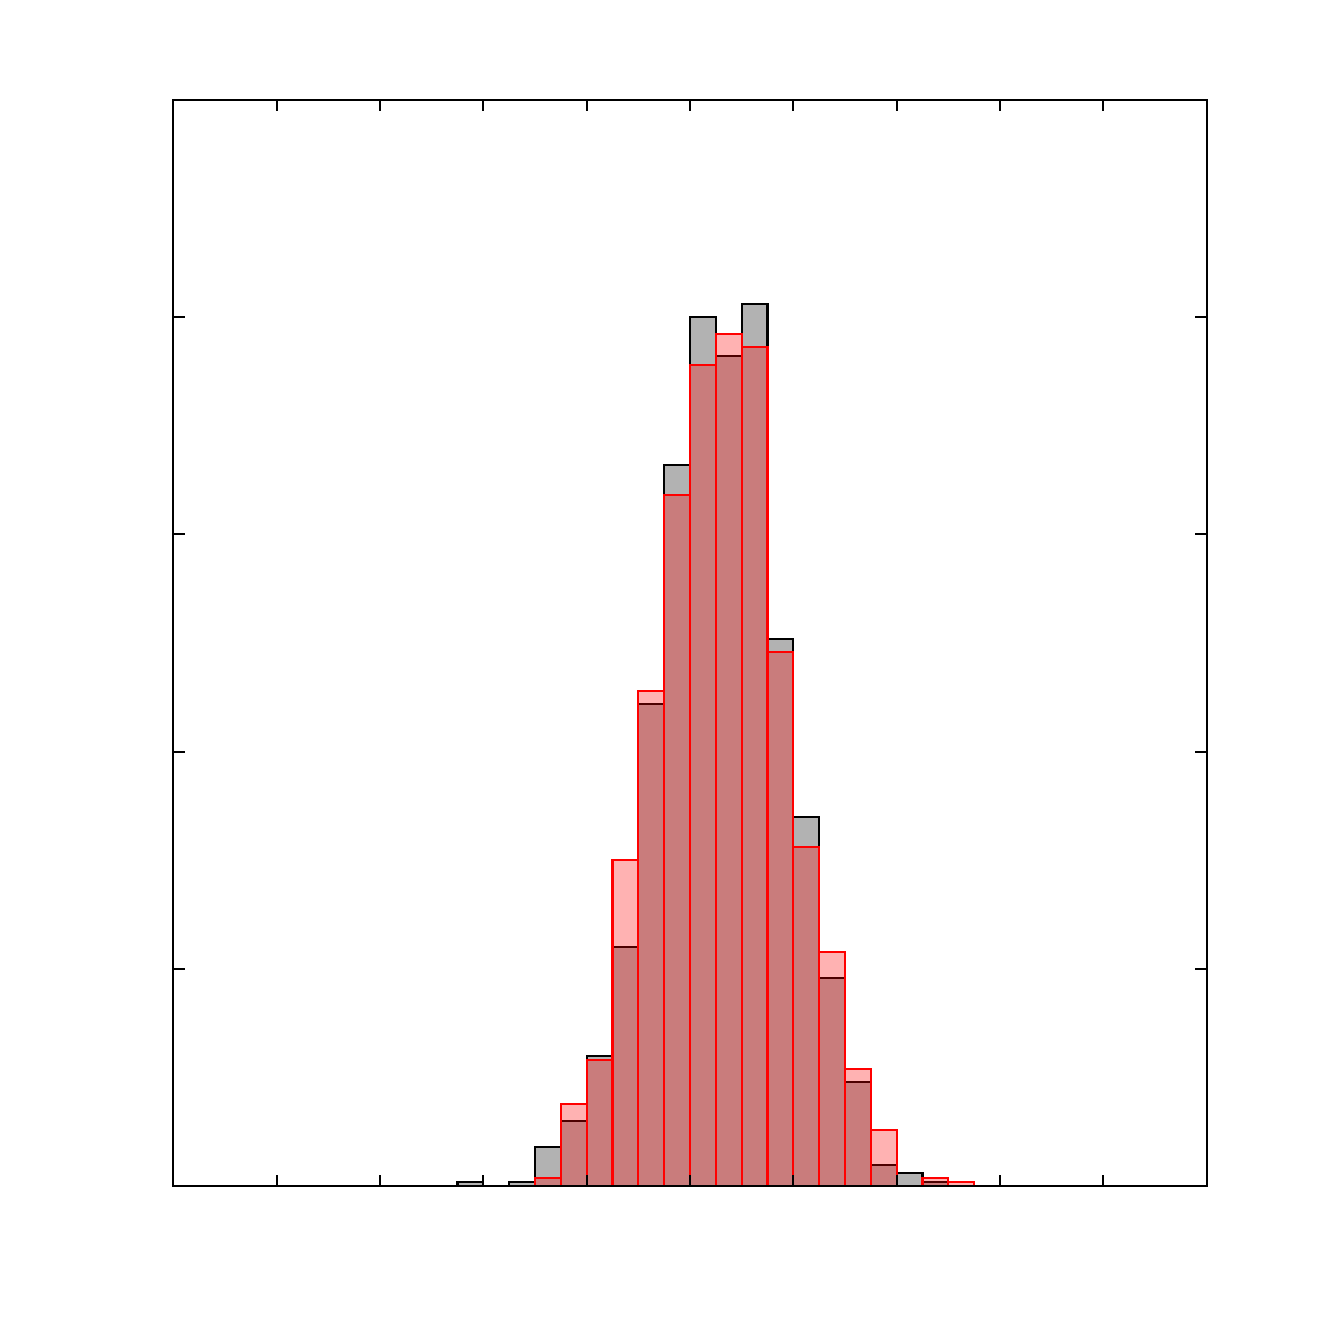
\includegraphics[width=0.47\linewidth]{figs/decoding/rcoef_sess_histallover_v1_blanco.pdf}
%     }
%     ~~
%     \subfloat[][\label{fig:noise_r_j1_hist}]{
%         \centering
% %         \includegraphics[width=0.47\linewidth]{%
% % ./rcoef_2013-03-25/rcoef_sess_histallover_2013-03-25/png/rcoef_sess_histallover_v1_jack.png}
%         \includegraphics[width=0.47\linewidth]{figs/decoding/rcoef_sess_histallover_v1_jack.pdf}
%     }
%     \\
%     \subfloat[][\label{fig:noise_r_b4_hist}]{
%         \centering
% %         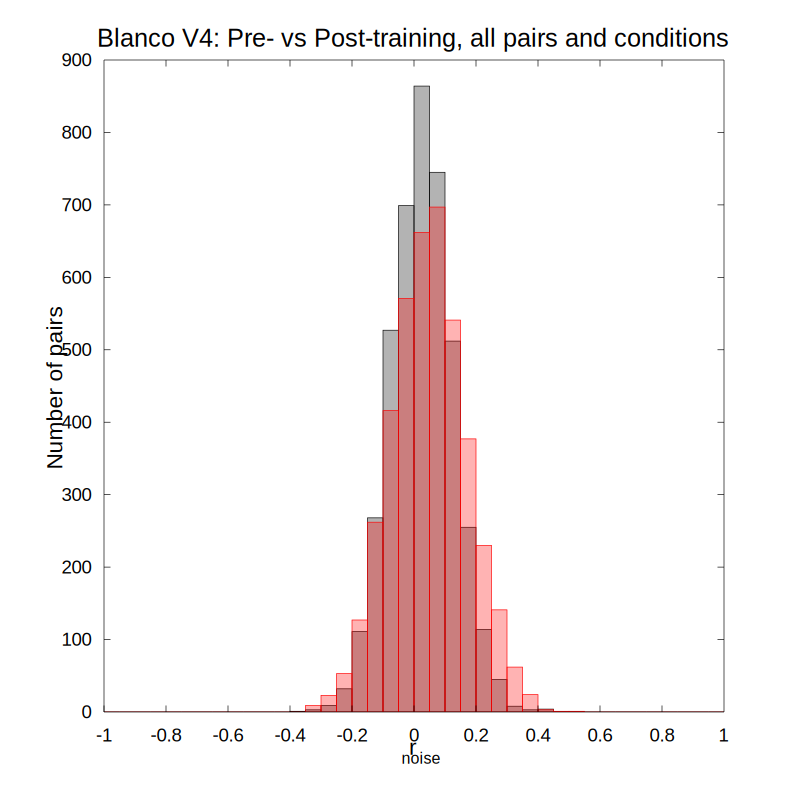
\includegraphics[width=0.47\linewidth]{%
% % ./rcoef_2013-03-25/rcoef_sess_histallover_2013-03-25/png/rcoef_sess_histallover_v4_blanco.png}
%         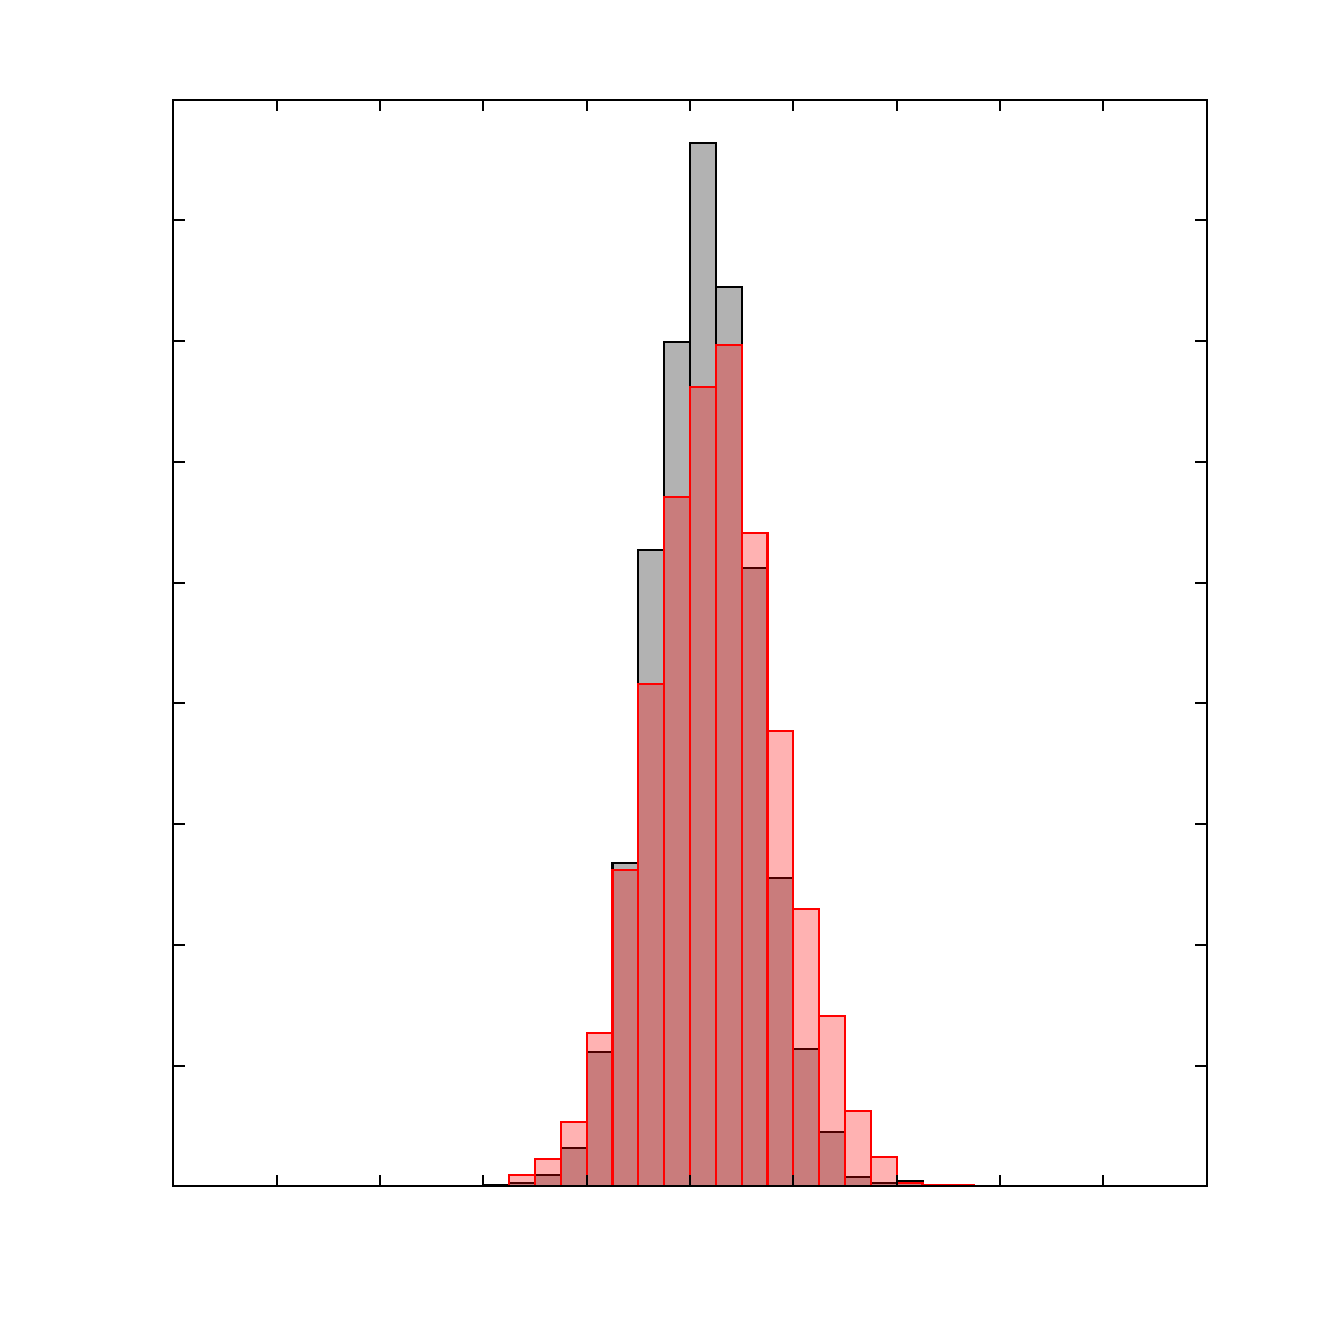
\includegraphics[width=0.47\linewidth]{figs/decoding/rcoef_sess_histallover_v4_blanco.pdf}
%     }
%     ~~
%     \subfloat[][\label{fig:noise_r_j4_hist}]{
%         \centering
% %         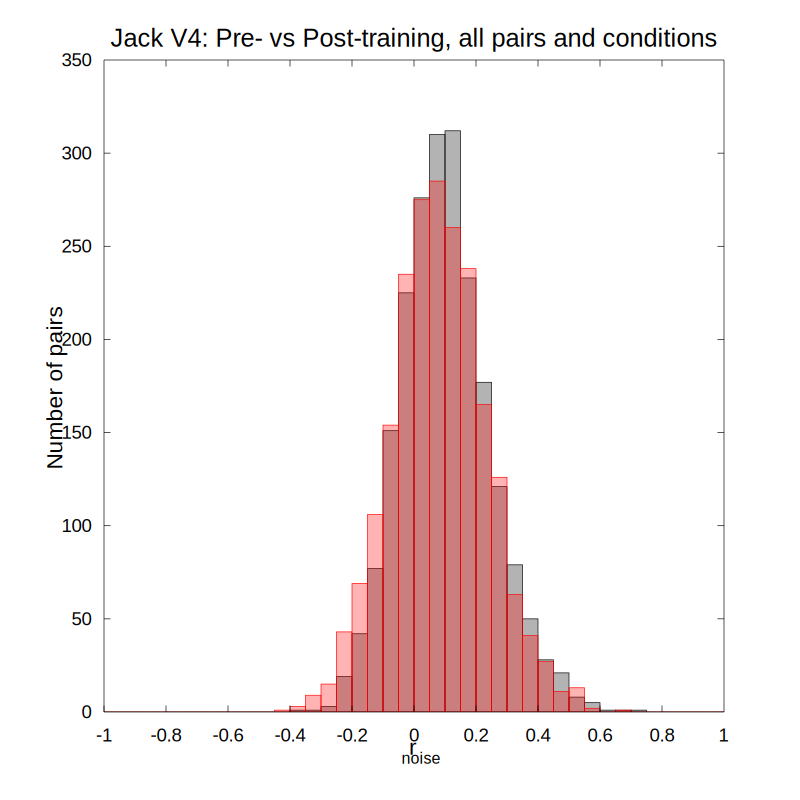
\includegraphics[width=0.47\linewidth]{%
% % ./rcoef_2013-03-25/rcoef_sess_histallover_2013-03-25/png/rcoef_sess_histallover_v4_jack.png}
%         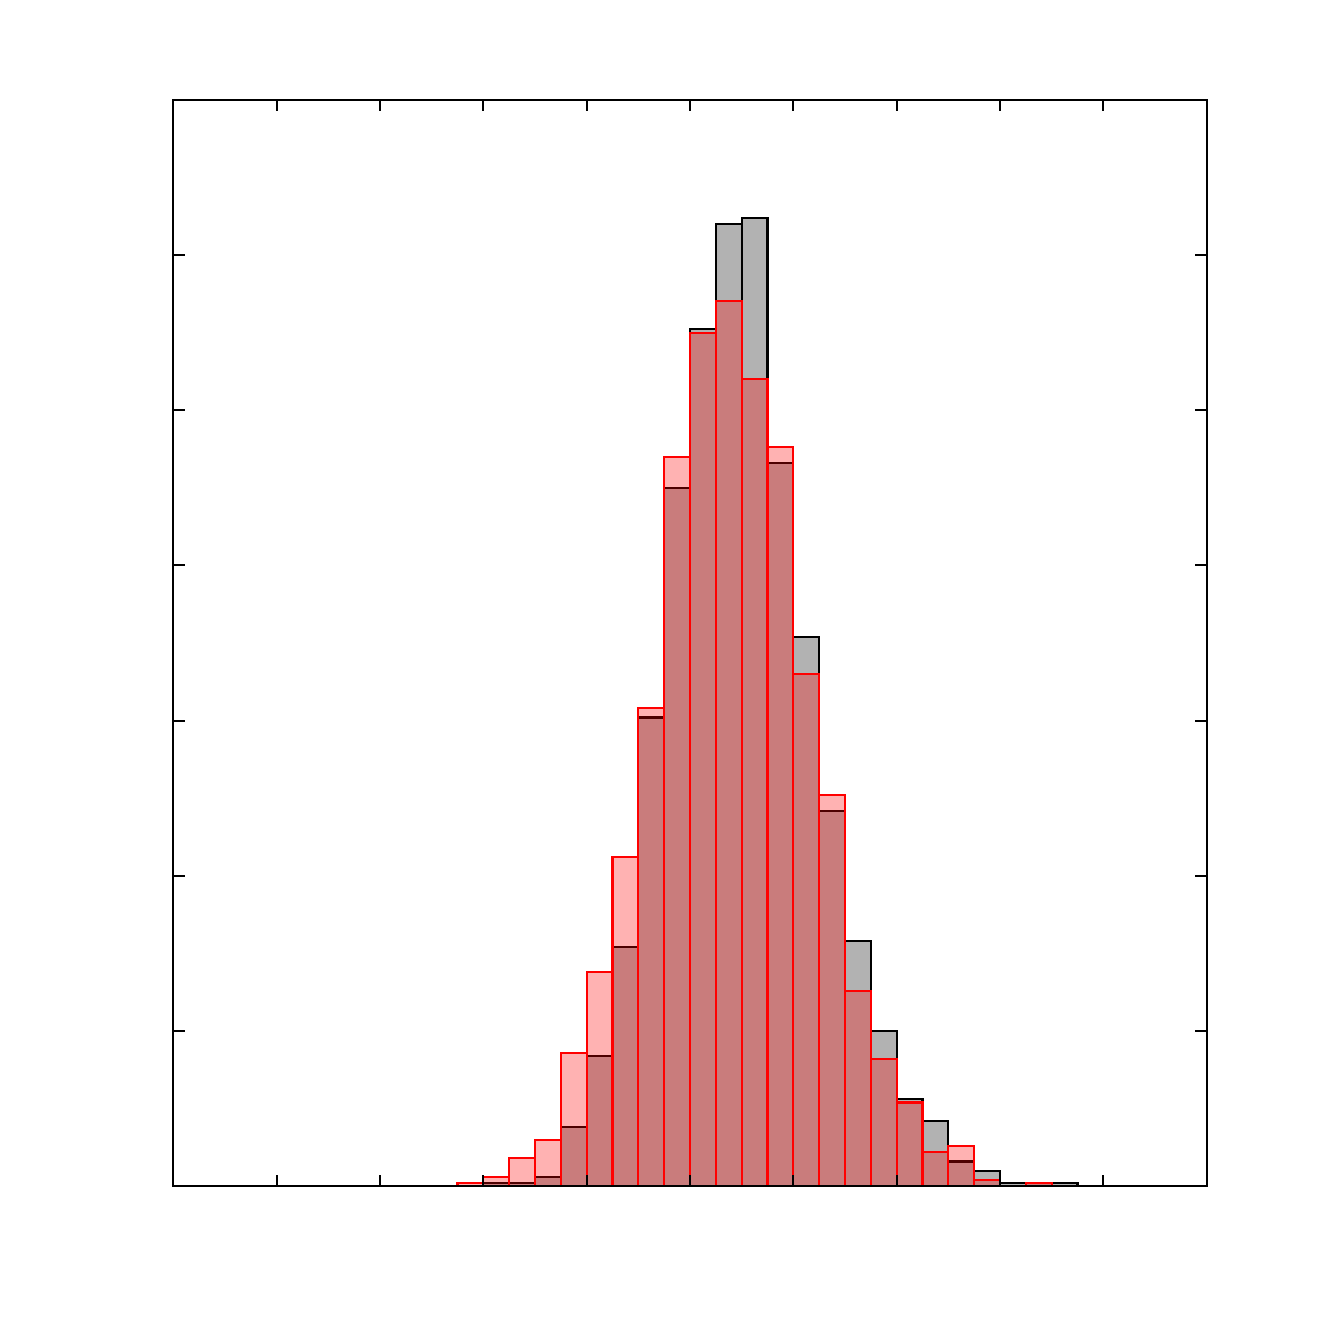
\includegraphics[width=0.47\linewidth]{figs/decoding/rcoef_sess_histallover_v4_jack.pdf}
%     }
%     \caption{Distribution of the noise correlations for the pairings across all conditions.
% Two sessions, one at the beginning of training (black) and one at the end of training (red) are shown for comparitive purposes.
% \protect\subref{fig:noise_r_b1_hist}: \ac{M1} \ac{V1}; sessions 343 and 354.
% \protect\subref{fig:noise_r_j1_hist}: \ac{M2} \ac{V1}; sessions 51 and 71.
% \protect\subref{fig:noise_r_b4_hist}: \ac{M1} \ac{V4}; sessions 307 and 338.
% \protect\subref{fig:noise_r_j4_hist}: \ac{M2} \ac{V4}; sessions 27 and 46.
% }
%     \label{fig:noise_r_hist}
% \end{figure}
%
%
% % \autoref{fig:noise_r_pmc} indicates that noise correlations are correlated for pairs across sessions.
% A pairs of channels which have higher noise correlations in one session are likely to have higher noise correlation in other sessions.
% However, this effect is not present for \ac{M1} \ac{V1}, \autoref{fig:noise_r_b1_pmc}, and could suggest there is less session-to-session consistency for this dataset.
%
% This figure provides an easy way of visually inspecting whether noise correlations are conserved, but does not allow us to quantify this.
%
% \begin{figure}[htbp]
%     \subfloat[][\label{fig:noise_r_b1_pmc}]{
%         \centering
%         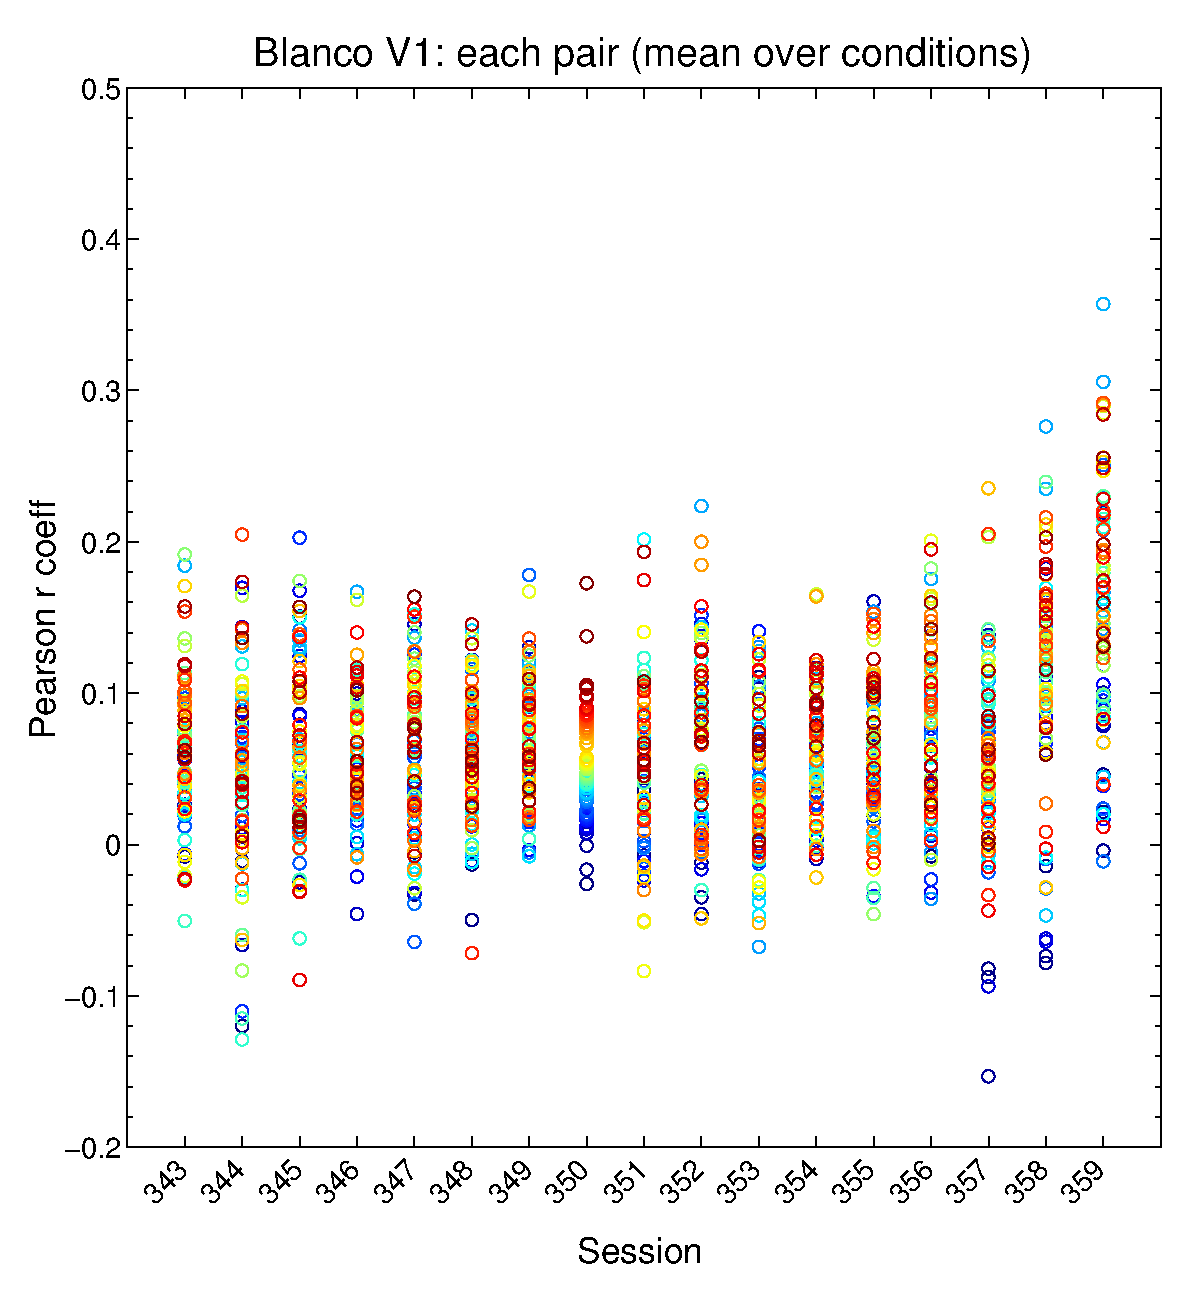
\includegraphics[width=0.47\linewidth]{%
% figs/decoding/rcoef_sess_pairsmeanc_v1_blanco.eps}
%     }
%     ~~
%     \subfloat[][\label{fig:noise_r_j1_pmc}]{
%         \centering
%         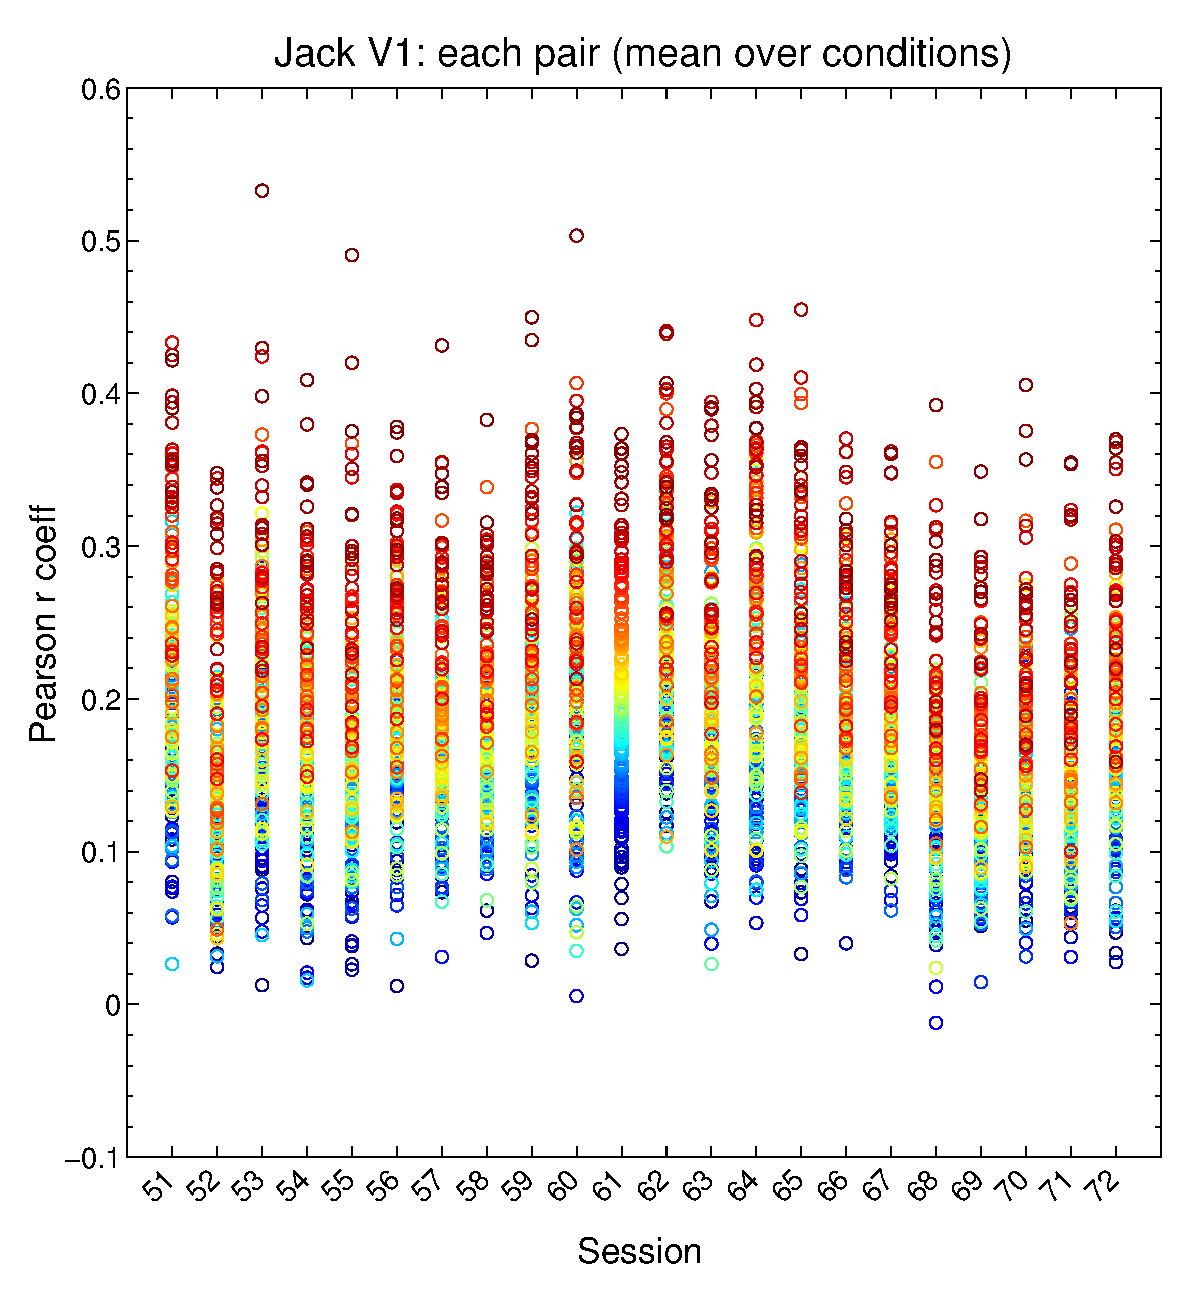
\includegraphics[width=0.47\linewidth]{%
% figs/decoding/rcoef_sess_pairsmeanc_v1_jack.eps}
%     }
%     \\
%     \subfloat[][\label{fig:noise_r_b4_pmc}]{
%         \centering
%         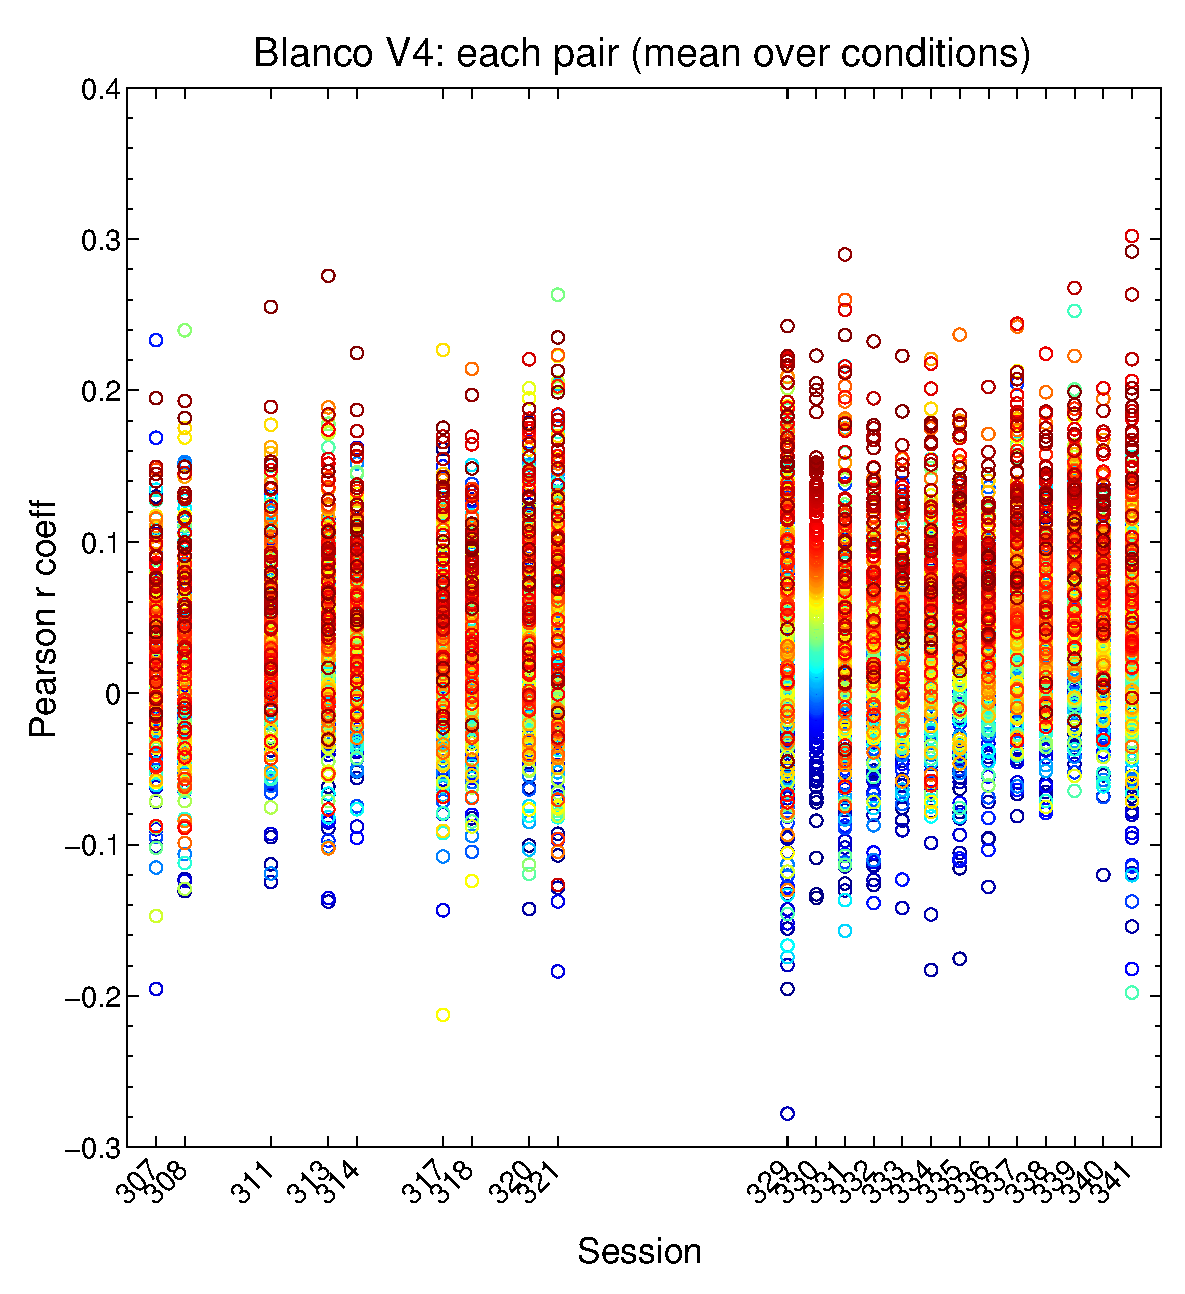
\includegraphics[width=0.47\linewidth]{%
% figs/decoding/rcoef_sess_pairsmeanc_v4_blanco.eps}
%     }
%     ~~
%     \subfloat[][\label{fig:noise_r_j4_pmc}]{
%         \centering
%         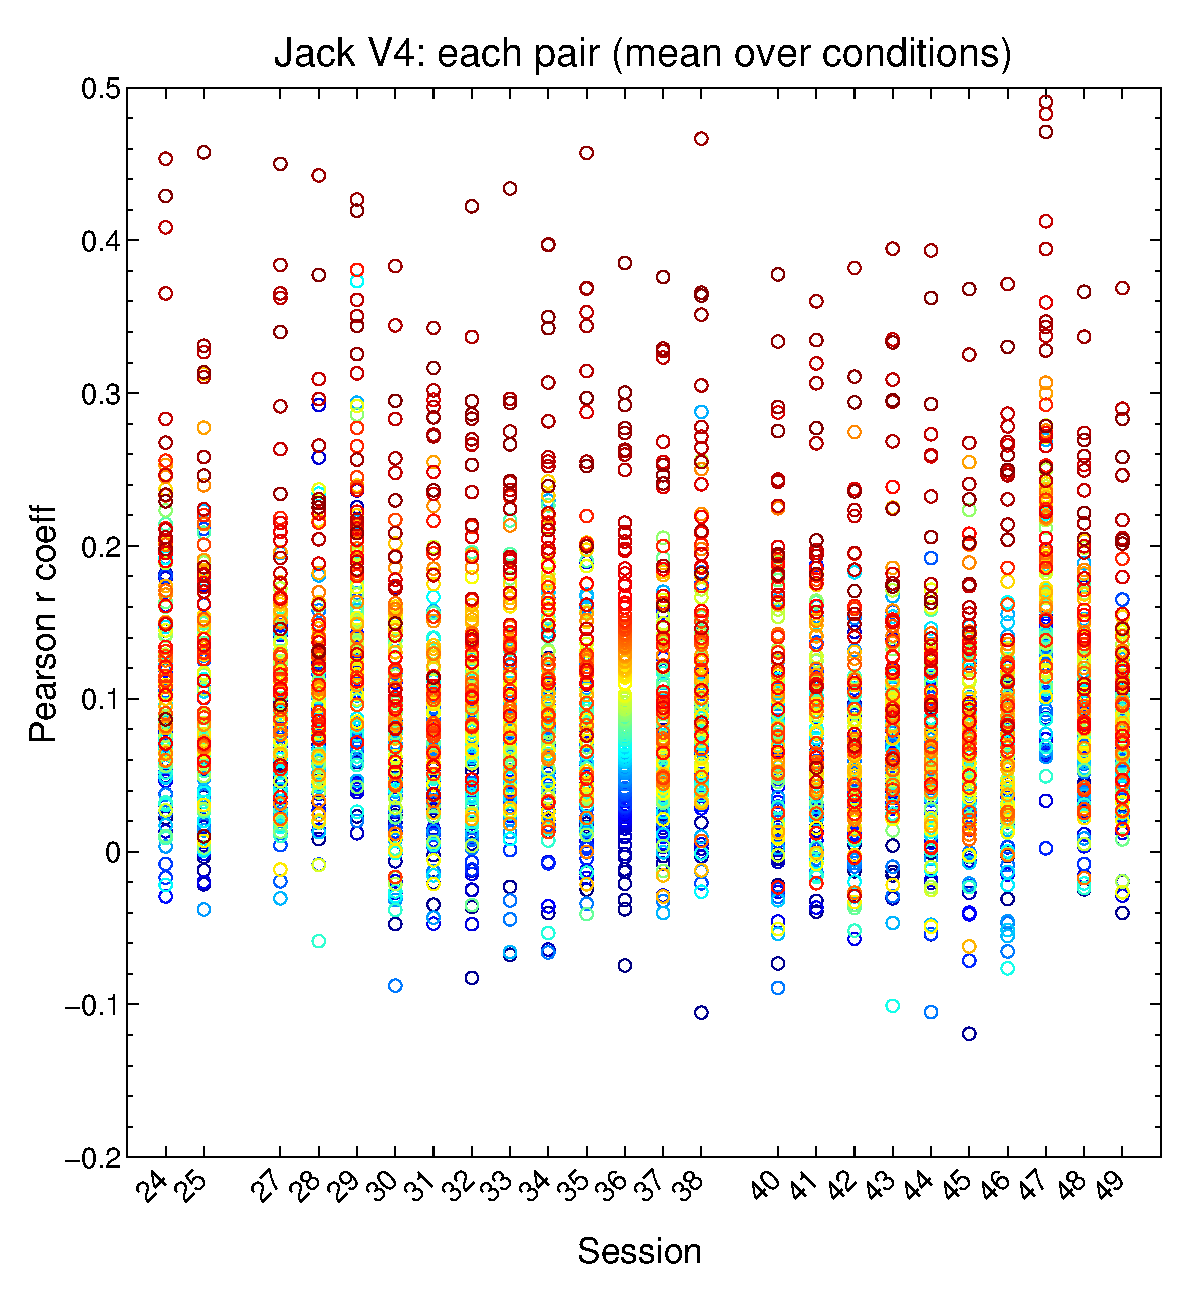
\includegraphics[width=0.47\linewidth]{%
% figs/decoding/rcoef_sess_pairsmeanc_v4_jack.eps}
%     }
%     \caption{Noise correlations for each pair, meaned across the 14 conditions.
% \protect\subref{fig:noise_r_b1_pmc}: \ac{M1} \ac{V1}.
% \protect\subref{fig:noise_r_j1_pmc}: \ac{M2} \ac{V1}.
% \protect\subref{fig:noise_r_b4_pmc}: \ac{M1} \ac{V4}.
% \protect\subref{fig:noise_r_j4_pmc}: \ac{M2} \ac{V4}.
% Colour is assigned by sorting the pairs into ascending order for one of the sessions near the middle of the training period.
% The degree of session-to-session correlation of the noise correlation can hence be inferred by visual inspection.
% }
%     \label{fig:noise_r_pmc}
% \end{figure}
%
%
%==============================================================================
\section{Sensitivity analysis}
%------------------------------------------------------------------------------

One simple method of comparing how the encoding of stimuli changes over time is to use the amount the sensitivity index, $d'$.
This gives a measure of how separable the signal and the noise are, by comparing the difference in their means with the overall standard deviation.
% For a classifier, this is defined as the difference between the hit rate and the false alarm rate,
% \begin{equation}
% d' = P(A | A) - P(A | \bar{A})
% ,\end{equation}

For Gaussian distributed data, the sensitivity index is defined as
\begin{equation}
d' = \frac{\mu_\text{stim} - \mu_\text{noise}}{\sigma_\text{joint}}
,\end{equation}
where the joint standard deviation is the over for the two distributions,
\begin{equation}
% \sigma_\text{joint} = \sqrt
%     \frac{ (n_\text{stim}-1) \, \sigma_\text{stim}^2 + (n_\text{noise}-1) \, \sigma_\text{noise}^2 }
%     { n_\text{stim} + n_\text{noise} - 2}
\sigma_\text{joint} = \sqrt \frac{\sigma_\text{stim}^2 + \sigma_\text{noise}^2}{2}
.\end{equation}
For our analysis, the noise is the spiking activity during periods of spontaneous activity.
With the sample stimulus and 14 test stimuli with differing contrast levels, we have 15 possible signals to choose from for each dataset.
Since it has the most presentations and lies in the middle of the range of the contrasts, we will just consider $d'$ with respect to the response signal when presenting the sample stimulus.

The number of spikes over a finite duration, which cannot be negative, is Poisson distributed instead of Gaussian distributed.
However, the two distributions do converge for large $n$, and so we disregard this and use the Gaussian form of the definition of $d'$.

%------------------------------------------------------------------------------
\subsection{Methods}

To compute $d'$, we considered the signal and noise to be the number of spikes occurring during a \SI{150}{\milli\second} period of activity.
For spontaneous (noise) activity, this was the \SI{150}{\milli\second} immediately preceding the sample stimulus onset.
For signal activity, this was the \SI{150}{\milli\second} either \SI{30}{\milli\second} (\ac{V1}) or \SI{60}{\milli\second} (\ac{V4}).
This delay was used to approximately account for the minimal possible response latency in \ac{V1} and \ac{V4}.

The violin plots showing the distribution over channels of $d'$ before and after training were created by taking a Gaussian kernel density with a bandwidth of 0.15.
This bandwidth was determined using the rule of thumb bandwidth estimator,
\begin{equation}
w = \hat{\sigma} \left( \frac{4}{3 n} \right) ^ \frac{1}{5}
,\end{equation}
for each animal and area on the distribution before and after training, and using the minimum of these 8 values.
This ensures sufficient detail about the distribution is captured for each distribution, and all are comparable with each other.

To investigate whether $d'$ changed significantly during the course of our experiments, we compared the average $d'$ during the first and final three experimental sessions (\zonename{A} and \zonename{B}).
A paired $t$-test (two-tailed) was used to study whether the $d'$ consistently increased or decreased for the channels.

%------------------------------------------------------------------------------
\subsection{\acs{V1} Results}

For \ac{V1}, we found the $d'$ decreased with training (see \autoref{fig:dprime_v1}).
A similar result was observed for each subject.
The average change in was $\Delta d' = -0.324$ ($p=0.02$, paired $t$-test) for \ac{M1} and $\Delta d' = -0.417$ ($p < 3 \times 10 ^{-10}$, paired $t$-test) for \ac{M2}.
 
\begin{figure}[htbp]
    \centering
    \hspace*{\fill}
    \subfloat[\ac{M1} \ac{V1}\label{fig:dprime_v1_blanco}]{
        \centering
        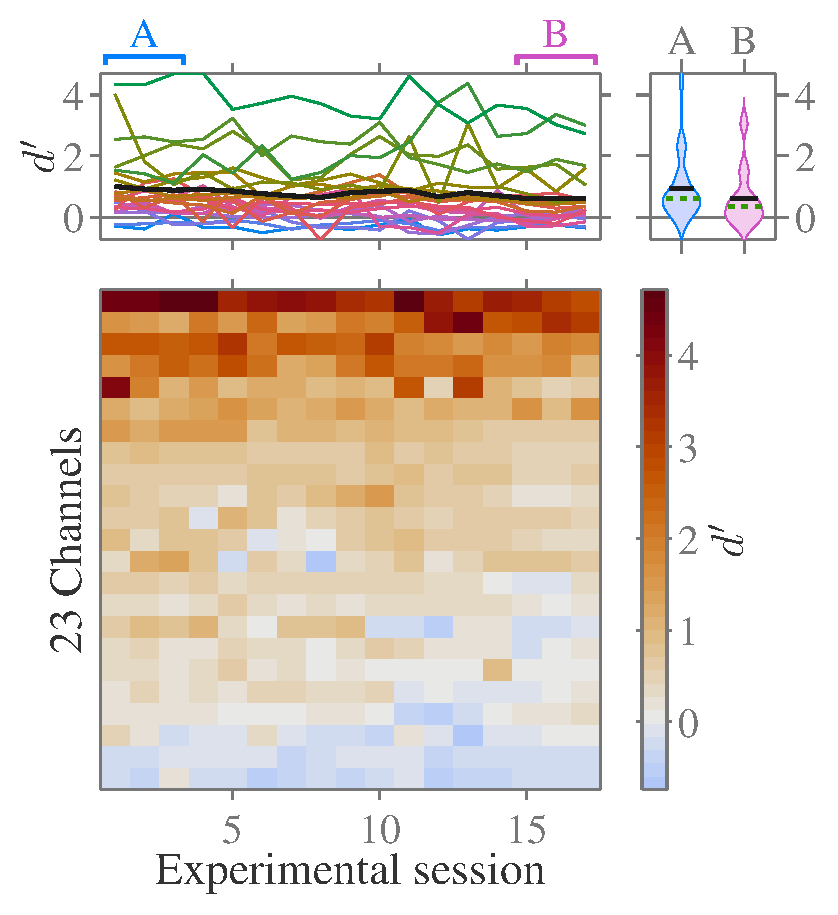
\includegraphics[scale=.45]{%
figs/dprime/dprime_sample_hm_hotcold_blanco_v1_1_rmon2_rmvet2.eps}
    }
    \hspace*{\fill}\hspace{.2cm}\hspace*{\fill}
    \subfloat[\ac{M2} \ac{V1}\label{fig:dprime_v1_jack}]{
        \centering
        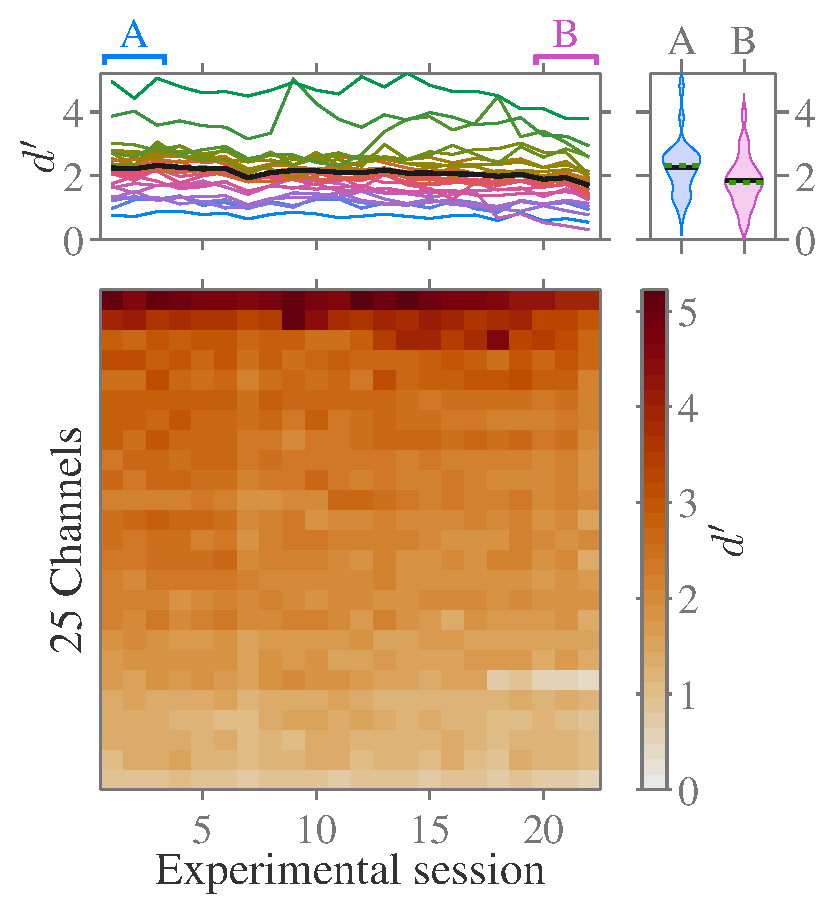
\includegraphics[scale=.45]{%
figs/dprime/dprime_sample_hm_hotcold_jack_v1_1_rmon2_rmvet2.eps}
    }
    \hspace*{\fill}
    \caption{Change in $d'$ over training sessions for \ac{V1} recordings.
\protect\subref{fig:dprime_v1_blanco}: $d'$ for \ac{M1}, shown for each recording channel, with channels ordered according to average $d'$ over all sessions.
Above, traces of $d'$ for each channel (colours), and average over channels (black).
Below, heatmap showing $d'$ for each channel.
Right top, violin plots showing distribution over channels of the average $d'$ in the first three sessions (\zonename{A}) and last three sessions (\zonename{B}), with mean (solid black line) and median (dashed green line) over channels indicated.
The violin plot shows a Gaussian kernel density using a bandwidth determined automatically as described in \autoref{sec:info-methods}.
\protect\subref{fig:dprime_v1_jack}: Same as \protect\subref{fig:dprime_v1_blanco}, but for \ac{M2}.
}
    \label{fig:dprime_v1}
\end{figure}


\subsection{\acs{V4} Results}
\label{sec:pl_dprime_v4}

This is in contrast with our findings for \ac{V4}.
For \ac{M1}, some channels marginally increased and others marginally decreased their $d'$ with training (\autoref{fig:dprime_v4_blanco}).
Overall, there was a small increase in average $d'$, with $\Delta d' = +0.053$, which was not a statistically significant change ($p=0.46$).

With \ac{M2}, many channels began training either indifferent to the stimulus, $d'=0$, or suppressed by it, $d'<0$ (\autoref{fig:dprime_v4_jack}).
Starting from this lower position, there was a significant increase of $\Delta d' = +0.491$ ($p < 7 \times 10 ^{-8}$).
However the final $d'$ for almost all channels recorded for \ac{M2} was still lower than the average $d'$ for \ac{M1}.

\begin{figure}[htbp]
    \centering
    \hspace*{\fill}
    \subfloat[\ac{M1} \ac{V4}\label{fig:dprime_v4_blanco}]{
        \centering
        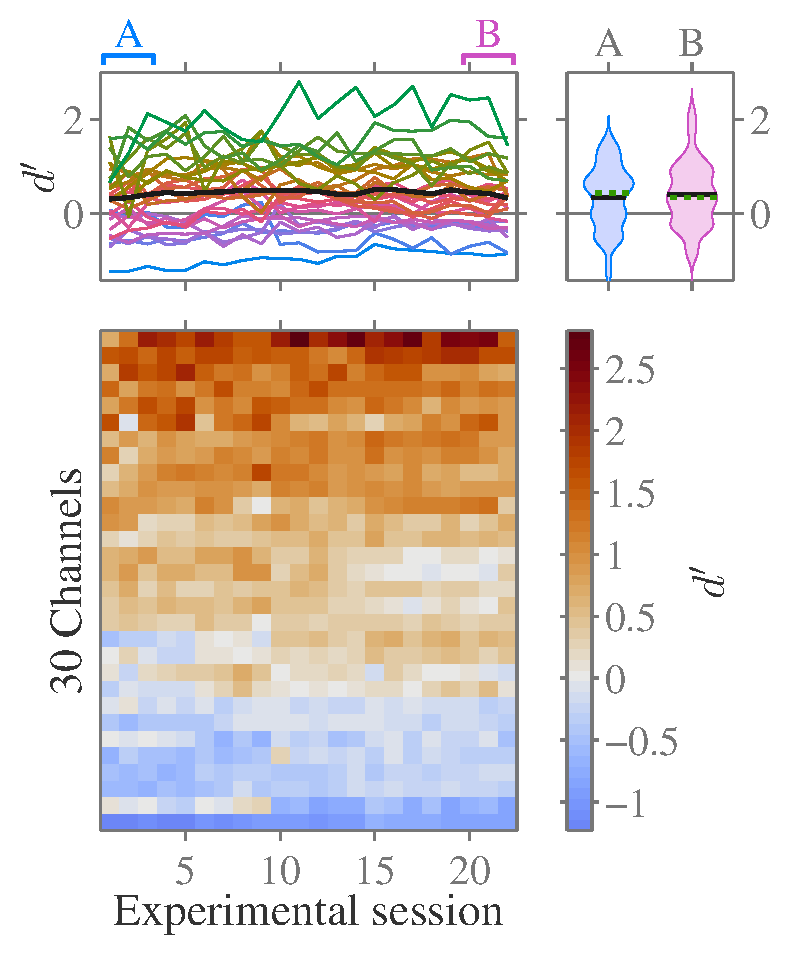
\includegraphics[scale=.45]{%
figs/dprime/dprime_sample_hm_hotcold_blanco_v4_1_rmon2_rmvet2.eps}
    }
    \hspace*{\fill}\hspace{.2cm}\hspace*{\fill}
    \subfloat[\ac{M2} \ac{V4}\label{fig:dprime_v4_jack}]{
        \centering
        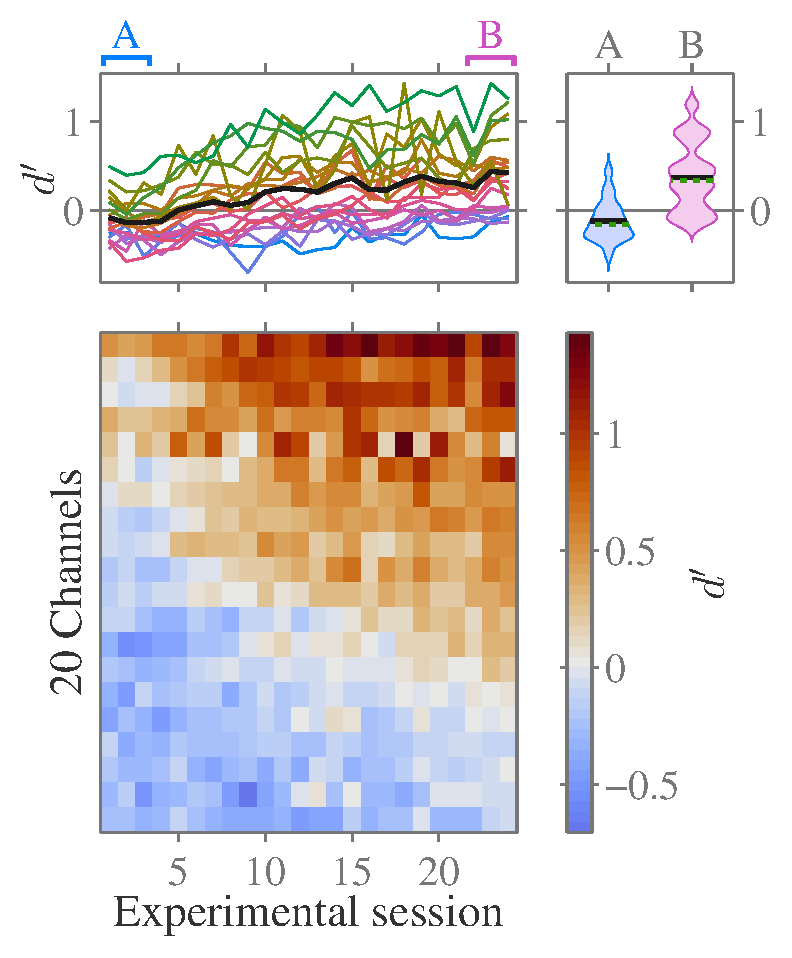
\includegraphics[scale=.45]{%
figs/dprime/dprime_sample_hm_hotcold_jack_v4_1_rmon2_rmvet2.eps}
    }
    \hspace*{\fill}
    \caption{Same as \autoref{fig:dprime_v1}, but for $d'$ during \ac{V4} recordings.
\protect\subref{fig:dprime_v4_blanco}: \ac{M1}.
\protect\subref{fig:dprime_v4_jack}: \ac{M2}.
}
    \label{fig:dprime_v4}
\end{figure}


\subsection{Discussion}
\label{sec:pl_dprime_discuss}

By analysing the sensitivity index, $d'$, we can see whether channels become more or less responsive to our stimulus class over time.
Since \ac{V1} is an early step in the visual processing hierarchy, its neurons respond strongly to simple stimuli such as the sinusoidal gratings we present.
Consequently, neurons have large responses to our stimuli even from the first session of the experimental training.
Over time, we found a decrease in sensitivity in \ac{V1} for both subjects.
We suspect this decrease in sensitivity of the neural response in \ac{V1} to the sample stimulus is due to unpreventable deterioration in the recording quality of the implanted chronic electrodes over time.
Overtime, the noise increases and the signal-to-noise ratio falls, which leads to a reduction in the distinguishability of the two activity distributions.

On the other hand, \ac{V4} is higher up the visual hierarchy and in general responds to more a complex stimulus class.
For \ac{M1}, many of the neurons we recorded from were responsive to the primitive Gabor stimulus from the beginning of training.
But for \ac{M2}, this was not the case --- on the contrary, many neurons were suppress by the Gabor stimulus.
With training, neurons recorded in \ac{M1} did not notably change their sensitivity to the sample stimulus, whereas $d'$ did increase for \ac{M2}.

We make particular note of the fact that the $d'$ in \ac{V4} increased for \ac{M2} from mostly negative initially values.
In principle, a decrease in activity in response to a stimulus can provide as much information about the presence of the stimulus as increase in activity.
However, it is difficult for neurons to increase their spontaneous activity due to the constraining effects of homeostasis, and it would be energetically inefficient for them to do so.
Therefore, since the firing rate of a neuron cannot fall below $0$ there is a smaller limit to the amount by which firing rates can differ if the information about the stimulus is conveyed by a reduction in activity compared to the background rate.
To provided more sensitivity for the response to our experimental stimuli, it thus makes sense for neurons which are suppressed by the stimulus class to increase their responses such that they are enhanced by its presence.
In practice, the de-suppression of the responses may arise not from the need of many individual neurons to encode the stimulus, but from a small number increasing the magnitude of their responses and then the connected neurons (which are positively correlated) increase their responses also.

From these results, we hypothesise that the sensitivity of the response to the experimental stimuli increases for the local network retinotopic to the stimulus location if it is too low for the network overall.
If the neurons are sufficiently sensitive to the stimulus to begin with (if $d'$ is high enough) then the sensitivity remains the same and does not increase with training.
Of course, the recorded sensitivity may decrease due to the decline in the recording quality.

With this measure, we can determine which channels contain neurons which change their relative responsiveness to the stimulus class, but we do not know how the distribution of responses change across the 14 different stimuli.
It is certainly plausible for neurons which begin their training already responsive to the stimuli to change their distribution of activity with respect to the contrast of the stimulus to provide more pertinent information for the experimental task.
For instance, this would be achieved if the absolute activity in response to the sample stimulus remains the same but the rate of change of activity with respect to the contrast of the stimulus increases.


%==============================================================================
\FloatBarrier
\section{Information in individual channels}
%------------------------------------------------------------------------------

We now apply the principles of Shannon information, as described in \autoref{sec:bgit}, to the perceptual learning data.
We are interested in how easy it is to determine which contrast the stimulus was presented with by observing the neural activity in response to the stimulus.
Since the subject's performance increases with training, we expect to find the amount of information encoded in the neural activity to increase with training.

To make its decision, the subject has access to all the neurons we have recorded and all the neurons in the brain from which we have not recorded.
Consequently, it would for the best idea of how much information the brain has access to, we would evaluate how much information is contained in the vector of neuronal responses for every recording channel.
However, this is problematic.
As the number of data streams combined into the response vector increases, the number of possible unique response vectors increases exponentially.
However, the number of trials recorded over is held fixed, and the number of possible response vectors must be constrained to prevent the estimated amount of information diverging to infinity (see \autoref{sec:bgit}).

Therefore, in this section we consider the information about the contrast of the stimulus encoded in the firing rate detected from only a single channel at once.
Because the spikes detected from each channel have been left unsorted and not resolved into clusters corresponding to individual neurons, this will be a multi-unit analysis, but only in the sense of neighbouring neurons being detected by the same electrode contact.


%------------------------------------------------------------------------------
\subsection{Methods}
\label{sec:info-methods}

The mutual information between the spiking activity during the presentation of the test stimulus and the identity of that stimulus was computed using the \textit{Information Breakdown Toolbox} for MATLAB \citep{Magri2009}.
Bias correction was performed using the \ac{PT} method (see \autoref{sec:bgit}) unless indicated otherwise.

The distribution of information over channels is shown using violin plots indicating the Gaussian kernel density with an automatically selected bandwidth.
We state the rule-of-thumb Gaussian basis bandwidth estimator as
\begin{equation}
h = \left( \frac{4}{3n} \right) ^ \frac{1}{5} \, \hat{\sigma}
,\label{eq:estimate-bw}\end{equation}
where $n$ is the number of samples and $\hat{\sigma}$ is the estimated standard deviation over the distribution.
We used \autoref{eq:estimate-bw} to find a suitable kernel basis bandwidth for the distribution over channels of information at the start (\zonename{A}) and end (\zonename{B}) of training.
For the plots, we selected the minimum of $\nicefrac{h_A}{2}$ and $\nicefrac{h_B}{2}$, to ensure sufficient detail was captured and the two distributions were comparable.

To test the significance of changes in information over time, we used a paired Student's $t$-test to compare the difference in information values in $\SET{\zonename{A}}$ and $\SET{\zonename{B}}$ against the null-hypothesis of no change between points \zonename{A} and \zonename{B}.
Although the distribution of information values is evidently non-Gaussian (it is bounded below at \SI{0}{bits}), the distribution in differences in information is close to Gaussian.
We could instead have used the Mann--Whitney $U$ test to compare the two distributions $\SET{\zonename{A}}$ and $\SET{\zonename{B}}$.
This test does not assume the two distributions are Gaussian, but makes the additional assumption that all samples are independent.
Since we record from the same set of channels for both $\SET{\zonename{A}}$ and $\SET{\zonename{B}}$, we are violating the independence assumption, and so the paired Student's $t$-test is a more appropriate choice.


%------------------------------------------------------------------------------
\subsection{Initial analysis}

First, we will consider the amount of information about the stimulus contained in a simple firing rate encoding.
For each test stimulus presentation, our response is the total number of spikes which were detected from a single channel during the first \SI{527}{\milli\second} of the stimulus presentation.%
\footnote{This duration is chosen because there is slight variation in the stimulus presentation time, and \SI{527}{\milli\second} is the shortest presentation duration.}

For each recording channel, we computed how much information was contained in this overall firing response about the identity of which stimulus had been presented.
The results of this initial analysis are shown in \autoref{fig:info_sess_1x527}.
We found that information in the overall firing rate of \ac{V1} channels increased with training for \ac{M2} (\SI{+0.069\pm0.017}{bits} or \SI{+16\pm5}{\percent} relative change, $p=0.0004$) but not for \ac{M1} (\SI{-0.051\pm0.029}{bits} or \SI{-34\pm19}{\percent}, $p=0.09$).
For \ac{V4}, there was an increase in information for both subjects however this increase was significant for \ac{M2} (\SI{+0.056\pm0.013}{bits} or \SI{+87\pm21}{\percent}, $p=0.0005$) but not \ac{M1} (\SI{+0.028\pm0.020}{bits} or \SI{+22\pm16}{\percent}, $p=0.17$).


\begin{figure}[htbp]%
    \centering
    \hspace*{\fill}
    \subfloat[][\ac{M1} \ac{V1}.\label{fig:info_sess_1x527_v1_blanco}]{%
        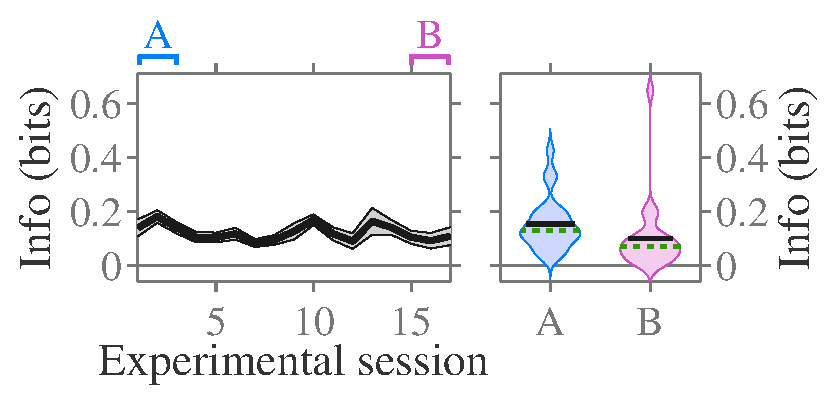
\includegraphics[scale=.45]{%
figs/info2/initial/I_sessionwise_blanco_v1_chmean23_s343-359_oc0_G_1bins_of_527ms_dr_pt_rmvet2_rmvms2_imscn_clhot.eps}}
    \hspace*{\fill}\hspace{.2cm}\hspace*{\fill}
    \subfloat[][\ac{M2} \ac{V1}.\label{fig:info_sess_1x527_v1_jack}]{%
        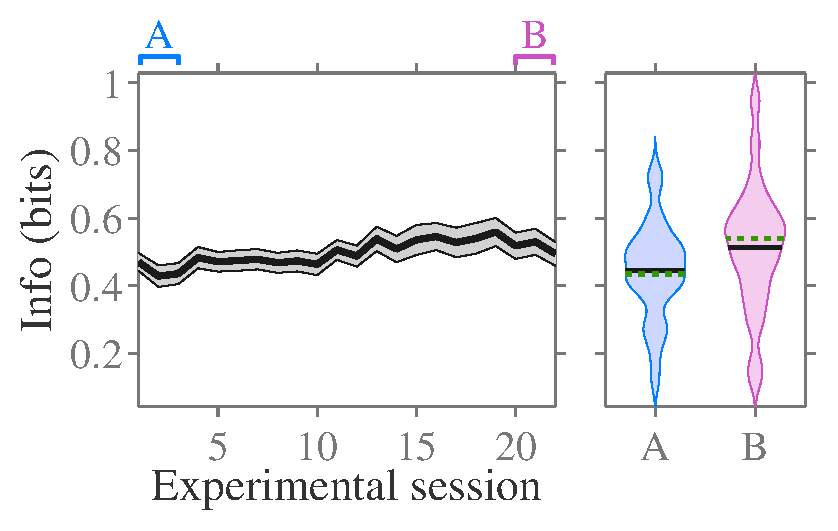
\includegraphics[scale=.45]{%
figs/info2/initial/I_sessionwise_jack_v1_chmean25_s51-72_oc0_G_1bins_of_527ms_dr_pt_rmvet2_rmvms2_imscn_clhot.eps}}
    \hspace*{\fill}
    \\
    \hspace*{\fill}
    \subfloat[][\ac{M1} \ac{V4}.\label{fig:info_sess_1x527_v4_blanco}]{%
        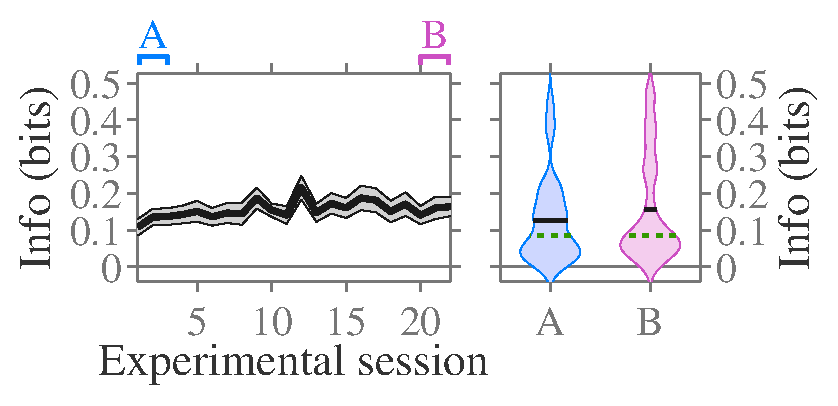
\includegraphics[scale=.45]{%
figs/info2/initial/I_sessionwise_blanco_v4_chmean30_s307,308,311,313,314,317,318,320,321,329-341_oc0_G_1bins_of_527ms_dr_pt_rmvet2_rmvms2_imscn_clhot.eps}}
    \hspace*{\fill}\hspace{.2cm}\hspace*{\fill}
    \subfloat[][\ac{M2} \ac{V4}.\label{fig:info_sess_1x527_v4_jack}]{%
        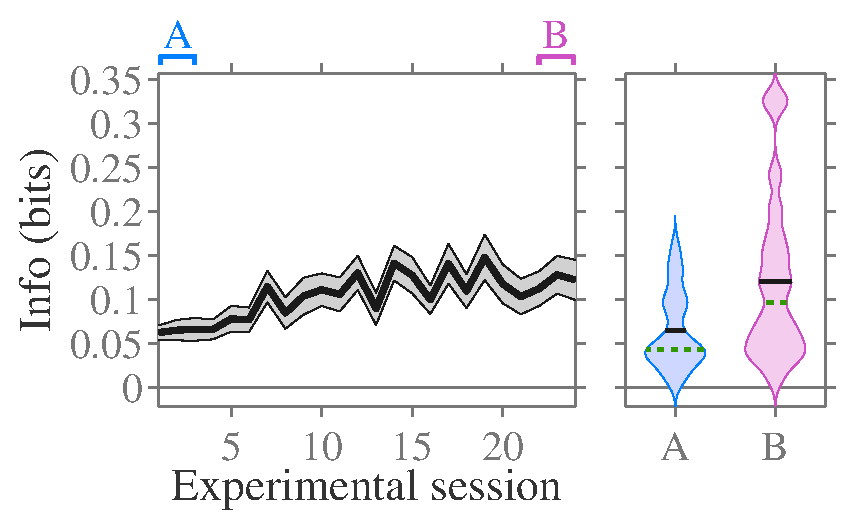
\includegraphics[scale=.45]{%
figs/info2/initial/I_sessionwise_jack_v4_chmean20_s24,25,27-38,40-49_oc0_G_1bins_of_527ms_dr_pt_rmvet2_rmvms2_imscn_clhot.eps}}
    \hspace*{\fill}
    \caption{Information about the test stimulus contained in the firing rate during test presentation and its progression over training sessions.
% The mutual information with the test stimulus is taken for a spike timing based code for a \SI{20}{ms} window of spiking activity, sampled with the start of the window offset ($y$-axis) from \SI{0}{ms} up to \SI{500}{ms} after test stimulus onset.
% The sampling is in intervals of \SI{5}{ms}, so any 4 adjacent squares within each session are highly correlated.
% The recording session number for the data is given along the $x$-axis, and the number of days the animal has been trained for increases from left to right.
% Average mutual information across all the channels is denoted by the pseudo-colour of each of the rectangular patches, centred around the $(x,y)$ co-ordinate to which the measurement relates.
Main panels: the average over channels (\protect\subref{fig:info_sess_1x527_v1_blanco}~23 channels, \protect\subref{fig:info_sess_1x527_v1_jack}~$25$ channels, \protect\subref{fig:info_sess_1x527_v4_blanco}~30 channels, \protect\subref{fig:info_sess_1x527_v4_jack}~$20$ channels) with standard error over channels indicated by the shaded region.
Right hand panels: distribution over channels of the information contained in the first three sessions (\zonename{A}) versus last three sessions (\zonename{B}), with mean (solid black line) and median (dashed green line) over channels indicated.
The violin plot shows a Gaussian kernel density, using a bandwidth determined as described in \autoref{sec:info-methods}.
The \ac{PT} bias correction method was used, without further correction to the residual bias.
}
    \label{fig:info_sess_1x527}
\end{figure}


As described in \autoref{sec:pl_dprime_discuss}, the reduction of information witnessed for \ac{M1} \ac{V1} is most likely explained by the inescapable reduction of recording signal quality over time.
However, one channel had a large increase in information content against the trend observed for other channels on this electrode array (see \autoref{fig:info_sess_1x527_v1_blanco}, right panel).
This channel is one of a minority whose response profile changes completely between consecutive sessions, and so the sudden large increase in information is most likely due to a small movement in the electrode contact changing which neurons are measured in the data.
We address this discrepancy next.


%------------------------------------
\subsubsection{Removing inconsistent channels}

We noted that some channels were moving between sessions.
In general, it is just as likely for electrode contacts to move into locations where they are more informative as to move such that they are less informative.
However, to make the results more comparable across sessions, we chose to remove channels whose raster profile or overall firing rate in response to the \SI{30}{\percent} sample stimulus clearly changed from one session to the next.
We manually selected a small number of channels on this basis, and removed them from the analysis.
For each dataset, the number of channels included afterwards is indicated in \autoref{tab:nchannels_restricted}.


\begin{table}[bthp]
\begin{center}
\begin{tabular}{ccrr}
\toprule
Region  & Animal    & Channels before   & Channels after \\
\midrule
V1      & M1        & 23                & 14 \\
        & M2        & 25                & 20 \\
V4      & M1        & 30                & 25 \\
        & M2        & 20                & 18 \\
\bottomrule
\end{tabular}
\end{center}
\caption{Number of channels before and after restriction on the basis of consistent or smoothly changing firing rates across sessions.}
\label{tab:nchannels_restricted}
\end{table}


\begin{figure}[htbp]%
    \centering
    \hspace*{\fill}
    \subfloat[][\ac{M1} \ac{V1}.\label{fig:info_sess_1x527_restrictchn_v1_blanco}]{%
        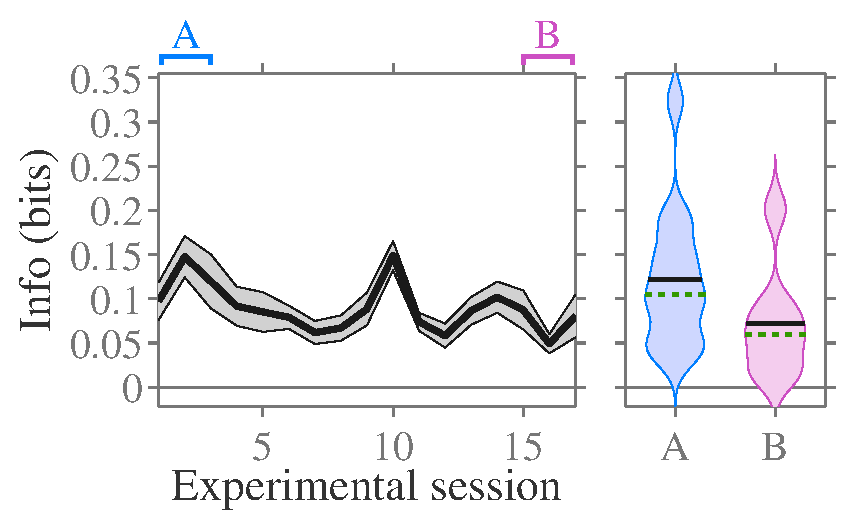
\includegraphics[scale=.45]{%
figs/info2/initial/I_sessionwise_blanco_v1_chmean14_s343-359_oc0_G_1bins_of_527ms_dr_pt_rmvet2_rmvms2_imscn_clhot.eps}}
    \hspace*{\fill}\hspace{.2cm}\hspace*{\fill}
    \subfloat[][\ac{M2} \ac{V1}.\label{fig:info_sess_1x527_restrictchn_v1_jack}]{%
        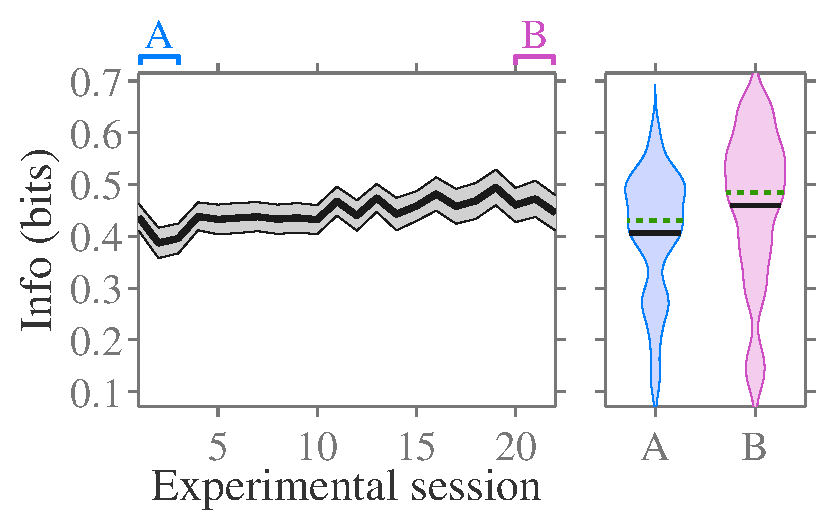
\includegraphics[scale=.45]{%
figs/info2/initial/I_sessionwise_jack_v1_chmean20_s51-72_oc0_G_1bins_of_527ms_dr_pt_rmvet2_rmvms2_imscn_clhot.eps}}
    \hspace*{\fill}
    \\
    \hspace*{\fill}
    \subfloat[][\ac{M1} \ac{V4}.\label{fig:info_sess_1x527_restrictchn_v4_blanco}]{%
        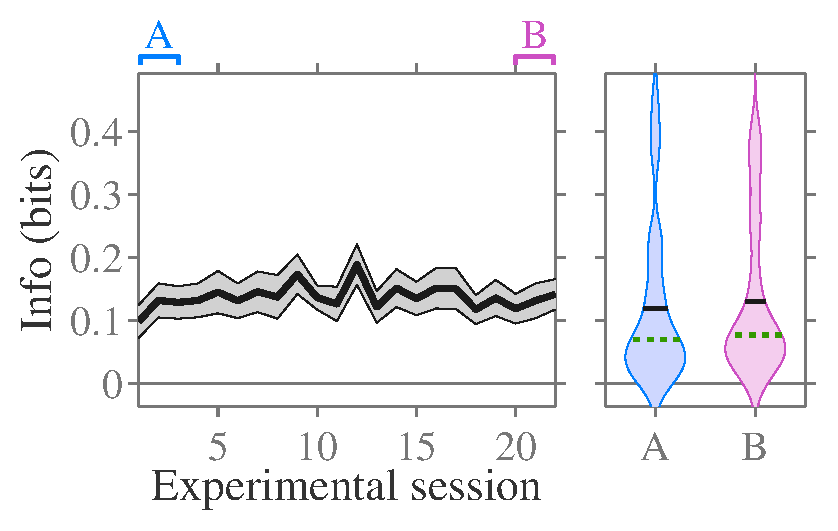
\includegraphics[scale=.45]{%
figs/info2/initial/I_sessionwise_blanco_v4_chmean25_s307,308,311,313,314,317,318,320,321,329-341_oc0_G_1bins_of_527ms_dr_pt_rmvet2_rmvms2_imscn_clhot.eps}}
    \hspace*{\fill}\hspace{.2cm}\hspace*{\fill}
    \subfloat[][\ac{M2} \ac{V4}.\label{fig:info_sess_1x527_restrictchn_v4_jack}]{%
        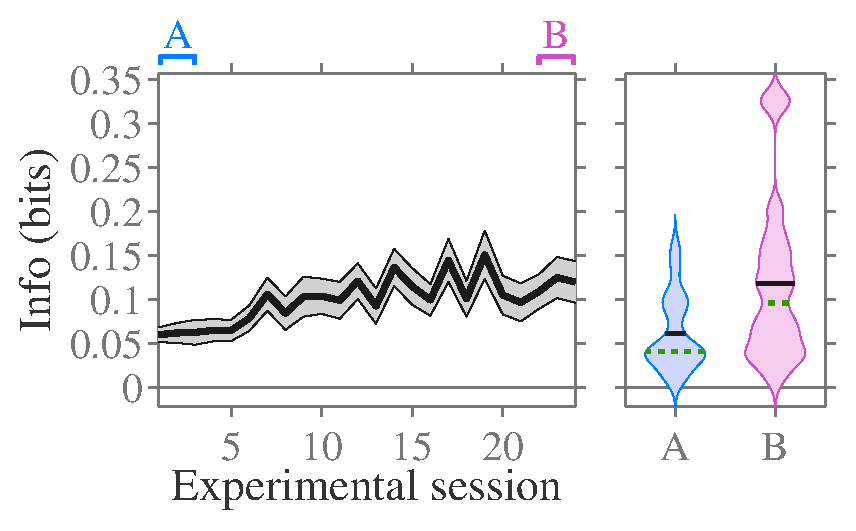
\includegraphics[scale=.45]{%
figs/info2/initial/I_sessionwise_jack_v4_chmean18_s24,25,27-38,40-49_oc0_G_1bins_of_527ms_dr_pt_rmvet2_rmvms2_imscn_clhot.eps}}
    \hspace*{\fill}
    \caption{Information about the test stimulus contained in the firing rate during test presentation and its progression over training sessions.
Main panels: the average over channels (\protect\subref{fig:info_sess_1x527_restrictchn_v1_blanco}~$14$ channels, \protect\subref{fig:info_sess_1x527_restrictchn_v1_jack}~$20$ channels, \protect\subref{fig:info_sess_1x527_restrictchn_v4_blanco}~$25$ channels, \protect\subref{fig:info_sess_1x527_restrictchn_v4_jack}~$18$ channels) with standard error over channels indicated by the shaded region.
Right hand panels: distribution over channels of the information contained in the first three sessions (\zonename{A}) versus last three sessions (\zonename{B}), with mean (solid black line) and median (dashed green line) over channels indicated.
The violin plot shows a Gaussian kernel density, using a bandwidth determined as described in \autoref{sec:info-methods}.
The \ac{PT} bias correction method was used, without further correction to the residual bias.
}
    \label{fig:info_sess_1x527_restrictchn}
\end{figure}

% blanco v1 1x527.00ms
% dr pt
% same bandwidth bw = 0.018561 used for all cols
% h=1.000000  p=0.014856=1.485642e-02   delta = -0.049242+/-0.017549 = -40.514232%+/-14.587530%
%
% jack v1 1x527.00ms
% dr pt
% same bandwidth bw = 0.033931 used for all cols
% h=1.000000  p=0.000970=9.696090e-04   delta = +0.052784+/-0.013545 = +12.980690%+/-4.272728%
%
% blanco v4 1x527.00ms
% dr pt
% same bandwidth bw = 0.033252 used for all cols
% h=0.000000  p=0.556266=5.562658e-01   delta = +0.010819+/-0.018130 = +9.059702%+/-15.387211%
%
% jack v4 1x527.00ms
% dr pt
% same bandwidth bw = 0.012428 used for all cols
% h=1.000000  p=0.001046=1.046127e-03   delta = +0.056465+/-0.014315 = +91.889667%+/-23.318749%

Besides the channel for \ac{M1} \ac{V1} with an aberrantly large increase in information mentioned above, there is little impact on the results (\autoref{fig:info_sess_1x527_restrictchn}) compared with previously (\autoref{fig:info_sess_1x527}).
For this dataset, \ac{M1} \ac{V1}, the removal of the outlier means the reduction in information over time is now statistically significant (\SI{-0.049\pm0.018}{bits} or \SI{-41\pm15}{\percent}, $p=0.015$).
For the other datasets, there were no notable changes.


%------------------------------------
\subsubsection{Correcting for stimulus class imbalance}
\label{sec:pl_class_imbalance}

As mentioned in \autoref{sec:pl_task}, the stimulus presentation procedure was to include a fixed number of repetitions of each stimulus in a block of trials and present them in a random order.
At the end of each block, additional trials were presented for stimuli which the subject responded to incorrectly.
Since stimuli with a contrast far from the pedestal contrast of \SI{30}{\percent} are much easier for the subject, trials which were repeated at the end of the block were not uniformly distributed across the stimuli.
Overall, this means that harder stimuli close to \SI{30}{\percent} contrast are presented more often than the easier stimuli.

When computing the amount of information about the stimulus contained in the animal's response, we do not need to have a uniform distribution across stimuli.
However, the subject becomes better at the task with training, and the change in relative performance is not uniform across sessions.
Performance on the easiest stimuli is high at the beginning of training and has little room for further improvements.
The hardest stimuli are very challenging, and performance on these does not rise much above chance even after training.
The increase in performance is highest for the stimuli of intermediate difficulty, and so since their first-try success rate improves they represent a smaller proportion of the total trials after training.

FIGURE SHOWING CHANGE IN CLASS BALANCE OVER TIME

Changes in the distribution of classes between sessions can impact our analysis in two ways.
Firstly, as described \autoref{eq:info} the amount of information between stimulus, $\SET{S}$, and response, $\SET{R}$, is dependent on the entropy of the stimulus, $\HH(\SET{S})$.
As the distribution of stimulus classes moves closer to uniform, the stimulus entropy increases.
Since our stimulus distribution becomes flatter with training, this may cause an the measured information to become inflated as training progresses.
Secondly, the proportion trials which are in the easier categories increases over time.
These stimuli will have the most distinguishable responses, and their increasing prevalence in the dataset may also produce an artificial increase in information with training.

We corrected the class imbalance on a session-by-session basis by subsampling the trials for more frequent stimulus classes down to the frequency of the least common stimulus class.
The trials included in the subsample were selected at random across the set of trials for each stimulus, without replacement.


\begin{figure}[htbp]%
    \centering
    \hspace*{\fill}
    \subfloat[][\ac{M1} \ac{V1}.\label{fig:info_sess_1x527_balanced_v1_blanco}]{%
        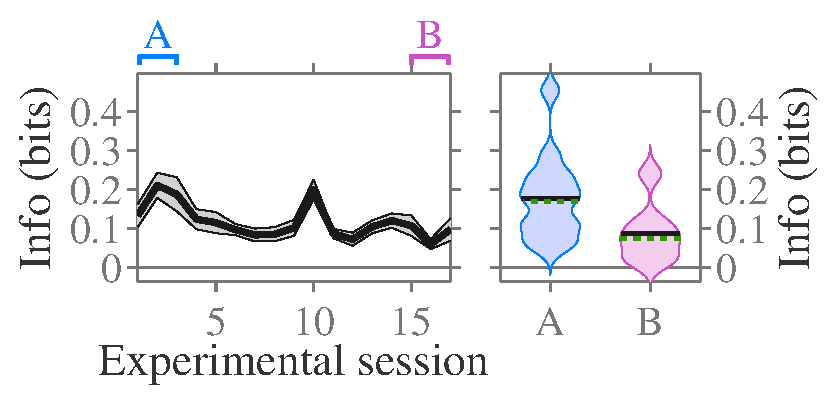
\includegraphics[scale=.45]{%
figs/info2/initial/I_sessionwise_blanco_v1_chmean14_s343-359_oc0_Gbalanced_1bins_of_527ms_dr_pt_rmvet2_rmvms2_imscn_clhot.eps}}
    \hspace*{\fill}\hspace{.2cm}\hspace*{\fill}
    \subfloat[][\ac{M2} \ac{V1}.\label{fig:info_sess_1x527_balanced_v1_jack}]{%
        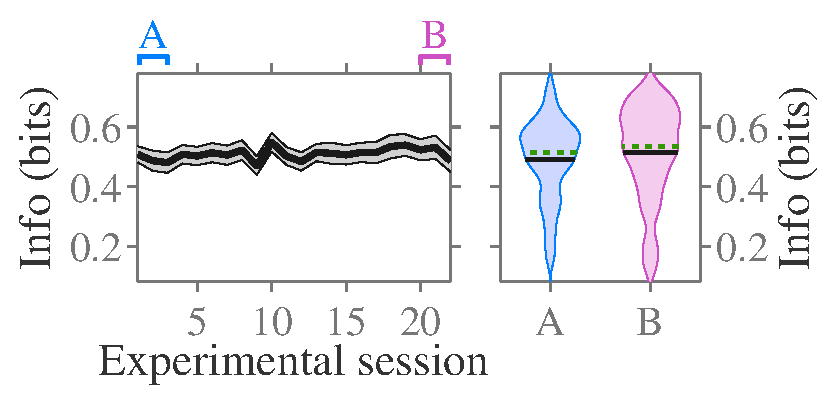
\includegraphics[scale=.45]{%
figs/info2/initial/I_sessionwise_jack_v1_chmean20_s51-72_oc0_Gbalanced_1bins_of_527ms_dr_pt_rmvet2_rmvms2_imscn_clhot.eps}}
    \hspace*{\fill}
    \\
    \hspace*{\fill}
    \subfloat[][\ac{M1} \ac{V4}.\label{fig:info_sess_1x527_balanced_v4_blanco}]{%
        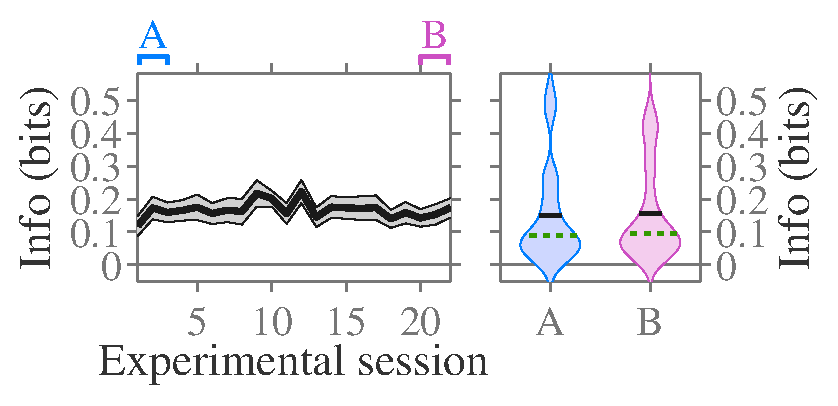
\includegraphics[scale=.45]{%
figs/info2/initial/I_sessionwise_blanco_v4_chmean25_s307,308,311,313,314,317,318,320,321,329-341_oc0_Gbalanced_1bins_of_527ms_dr_pt_rmvet2_rmvms2_imscn_clhot.eps}}
    \hspace*{\fill}\hspace{.2cm}\hspace*{\fill}
    \subfloat[][\ac{M2} \ac{V4}.\label{fig:info_sess_1x527_balanced_v4_jack}]{%
        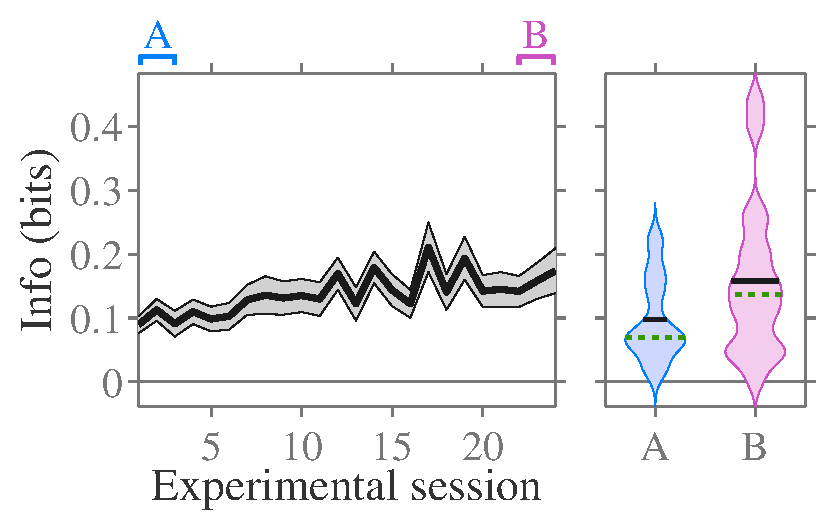
\includegraphics[scale=.45]{%
figs/info2/initial/I_sessionwise_jack_v4_chmean18_s24,25,27-38,40-49_oc0_Gbalanced_1bins_of_527ms_dr_pt_rmvet2_rmvms2_imscn_clhot.eps}}
    \hspace*{\fill}
    \caption{Information about the test stimulus contained in the firing rate during test presentation and its progression over training sessions, after correcting for the stimulus class balance in each session.
Main panels: the average over channels (\protect\subref{fig:info_sess_1x527_balanced_v1_blanco}~$14$ channels, \protect\subref{fig:info_sess_1x527_balanced_v1_jack}~$20$ channels, \protect\subref{fig:info_sess_1x527_balanced_v4_blanco}~$25$ channels, \protect\subref{fig:info_sess_1x527_balanced_v4_jack}~$18$ channels) with standard error over channels indicated by the shaded region.
Right hand panels: distribution over channels of the information contained in the first three sessions (\zonename{A}) versus last three sessions (\zonename{B}), with mean (solid black line) and median (dashed green line) over channels indicated.
The violin plot shows a Gaussian kernel density, using a bandwidth determined as described in \autoref{sec:info-methods}.
The \ac{PT} bias correction method was used, without further correction to the residual bias.
}
    \label{fig:info_sess_1x527_balanced}
\end{figure}

% blanco v1 1x527.00ms
% dr pt
% same bandwidth bw = 0.02234 used for all cols
% h=1.000000  p=0.001794=1.794017e-03   delta = -0.089123+/-0.022797 = -50.472174%+/-13.226381%
%
% jack v1 1x527.00ms
% dr pt
% same bandwidth bw = 0.038202 used for all cols
% h=0.000000  p=0.179003=1.790031e-01   delta = +0.022181+/-0.015896 = +4.511570%+/-4.419345%
%
% blanco v4 1x527.00ms
% dr pt
% same bandwidth bw = 0.038581 used for all cols
% h=0.000000  p=0.779391=7.793914e-01   delta = +0.006273+/-0.022144 = +4.185196%+/-15.076193%
%
% jack v4 1x527.00ms
% dr pt
% same bandwidth bw = 0.018676 used for all cols
% h=1.000000  p=0.004131=4.130838e-03   delta = +0.060078+/-0.018145 = +61.470204%+/-18.627960%


Overall, we find the amount of information increases when the class imbalance is for (compare the y-scales of \autoref{fig:info_sess_1x527_balanced} with those of \autoref{fig:info_sess_1x527_restrictchn}).
This is because the stimulus entropy, $\HH(\SET{S})$, has increased when the stimulus distribution became uniform.

As anticipated, correcting for changes in the class balance over time reduces the relative increase in information between the beginning and end of training.
For \ac{V1}, the reduction in information with time seen in \ac{M1} is increased (\SI{-0.089\pm0.023}{bits} or \SI{-50\pm13}{\percent}, $p=0.0018$) and the increase in information for \ac{M2} is no longer statistically significant (\SI{+0.022\pm0.016}{bits} or \SI{+4.5\pm4.4}{\percent}, $p=0.18$).
For \ac{V4}, the outcomes stand unchanged even though the relative change in information is reduced
(\ac{M1}: \SI{+0.006\pm0.022}{bits} or \SI{+4\pm15}{\percent}, $p=0.78$; \ac{M2}: \SI{+0.060\pm0.018}{bits} or \SI{+61\pm19}{\percent}, $p=0.004$).


%------------------------------------
\subsubsection{Defending against changes in session duration}

A large amount of session-to-session variability in the measurements was observed in our results (\autoref{fig:info_sess_1x527}).
Further investigation revealed that this variability was due to changes in the duration of each session --- some sessions contain $5$ times as many trials as others.

Although we were utilising the \ac{PT} bias correction technique, this typically requires $4$ trials per response for each stimulus condition to be completely effective \citep{Panzeri2007}.
When analysing the amount of information contained in the overall firing rate, the cardinality of the set of spike counts per channel ranges from N to M.
The number of trials per session (including all 14 stimulus conditions) ranges from N to M. (250 to 1250, approx)
Consequently, the number of trials per stimulus ranges from N to M.
After correcting for the stimulus class imbalance, the effective number of trials per session ranges from N to M.

This shortage of trials per stimulus condition results means the \ac{PT} bias correction method underestimates the bias for the shorter sessions, leading to an overestimate in the reported information.
This is illustrated in \autoref{fig:I_vs_invN}, where we compare with the estimated information with the reciprocal number of trials, $\nicefrac{1}{N}$, and find a linear correlation.
This is in keeping with the literature, since $\I_{\text{measured}}$ is known to be proportional to $\nicefrac{1}{N}$ if no bias correction is performed \citep{Treves1995}.


\begin{figure}[htbp]
    \centering
    \hspace*{\fill}
    \subfloat[][\ac{M1} \ac{V1}.\label{fig:I_vs_invN_v1_blanco}]{%
        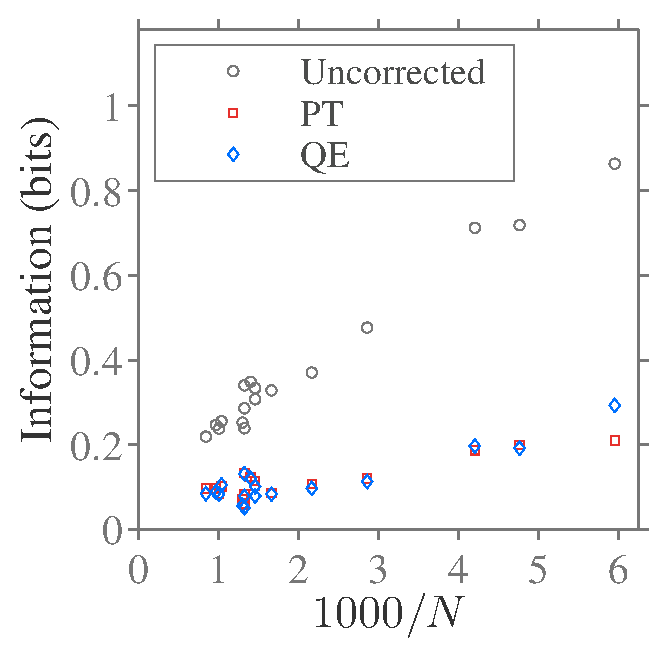
\includegraphics[scale=.45]{%
figs/info2/bias/ntrials_I_vs_invN_combindivpap_leg_blanco_v1_14chn_Gbalanced_1bins_of_527ms.eps}}
    \hspace*{\fill}\hspace{.2cm}\hspace*{\fill}
    \subfloat[][\ac{M2} \ac{V1}.\label{fig:I_vs_invN_v1_jack}]{%
        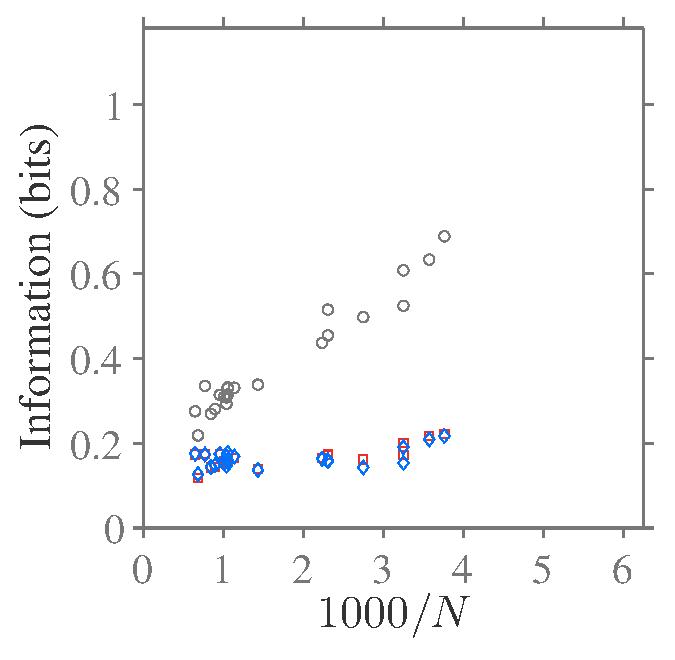
\includegraphics[scale=.45]{%
figs/info2/bias/ntrials_I_vs_invN_combindivpap_blanco_v4_25chn_Gbalanced_1bins_of_527ms.eps}}
    \hspace*{\fill}
    \\
    \hspace*{\fill}
    \subfloat[][\ac{M1} \ac{V4}.\label{fig:I_vs_invN_v4_blanco}]{%
        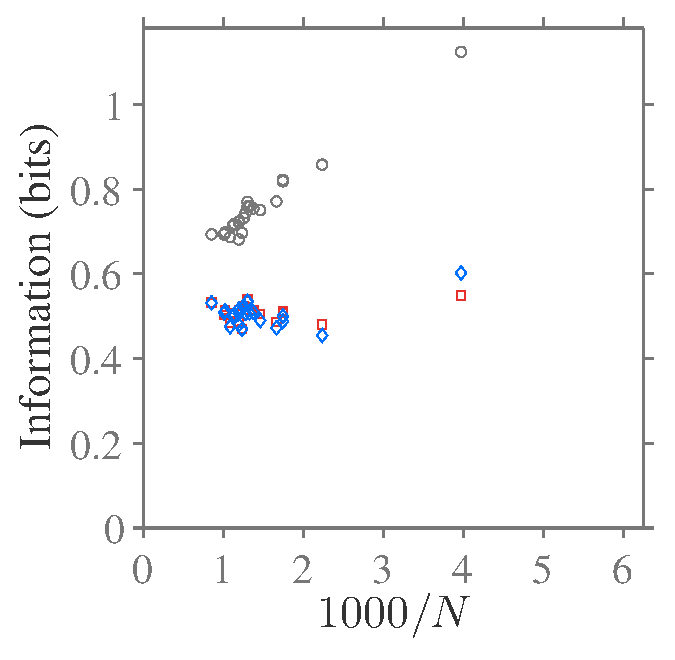
\includegraphics[scale=.45]{%
figs/info2/bias/ntrials_I_vs_invN_combindivpap_jack_v1_20chn_Gbalanced_1bins_of_527ms.eps}}
    \hspace*{\fill}\hspace{.2cm}\hspace*{\fill}
    \subfloat[][\ac{M2} \ac{V4}.\label{fig:I_vs_invN_v4_jack}]{%
        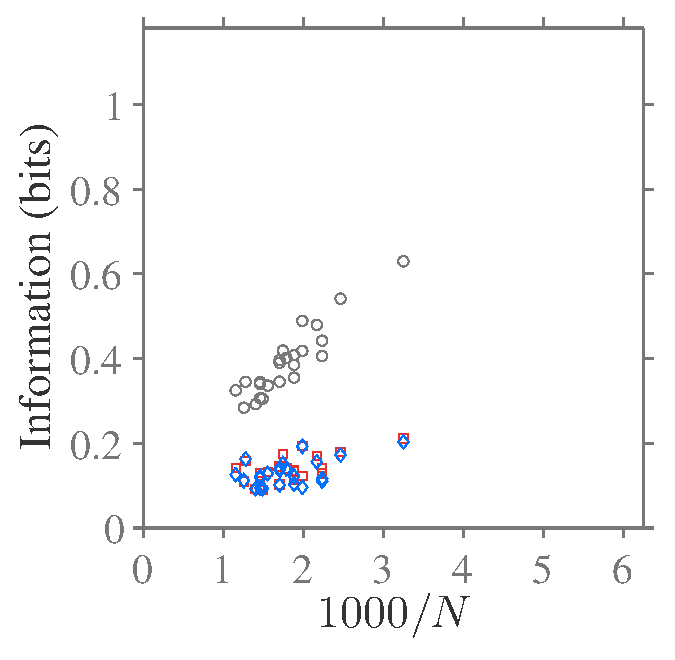
\includegraphics[scale=.45]{%
figs/info2/bias/ntrials_I_vs_invN_combindivpap_jack_v4_18chn_Gbalanced_1bins_of_527ms.eps}}
    \hspace*{\fill}
    \caption{Distribution of measured information as a function of $\nicefrac{1}{N}$, where $N$ is the number of trials in the session.
Results are shown both without correcting for the finite measurement bias (grey circles), using \ac{PT} bias correction (red squares), and using \ac{QE} bias correction (blue diamonds).
Information was computed after using subsampling to address the stimulus class imbalance (see \autoref{sec:pl_class_imbalance}), and this is reflected in the value of $N$.
}
    \label{fig:IvN}
    \label{fig:I_vs_invN}
\end{figure}


There are several potential ways we can correct for the change in bias incurred by the changes in number of trials.
\begin{itemize}
\item Subsample all sessions down to the same number of trials (rarefy).
\item Use bootstrapping, randomising the mapping between stimulus and response, to estimate the residual bias and subtract this from the reported information.
\item Group together stimuli above and below \SI{30}{\percent} contrast so we only two conditions each with approximately $7$ times more trials.
\item Group together trials across consecutive sessions so we have the same number of trials in each information computation step.
\end{itemize}

The first method is clearly undesirable, since we would be throwing away most of our data and knowingly operating in the regime where the bias correction method breaks down for all sessions instead of only a few.
In such a scenario, the bias on the estimated information would be larger than the actual information and our comparison across sessions would have little validity.
Instead, we focus on the three other more practical methods, whose outcomes are described below.


%------------------------------------
 \subsubsection{Bootstrap correction}
 \label{sec:pl_bootstrapping}

Shuffling the responses across stimuli destroys the information contained in the response about the stimulus.
By performing such shuffling and computing the amount of information between the randomly paired labels, we can estimate the bias \citep{Optican1991}.
Using this in conjunction with a bias correction technique such as \ac{PT} both when performing the original and bootstrapped information calculation allows us to estimate the residual bias after on the corrected value.
As described in \autoref{sec:info-bias} and by \citet{Panzeri1996}, this will typically lead to an overestimate of the bias.
However, since our residual bias will be significantly reduced beforehand due to the \ac{PT} technique, the overestimation is on a much smaller residual bias and impacts the results less.

\begin{figure}[htbp]
    \centering
    \hspace*{\fill}
    \subfloat[][\ac{M1} \ac{V1}.\label{fig:I_vs_invN_btsp_v1_blanco}]{%
        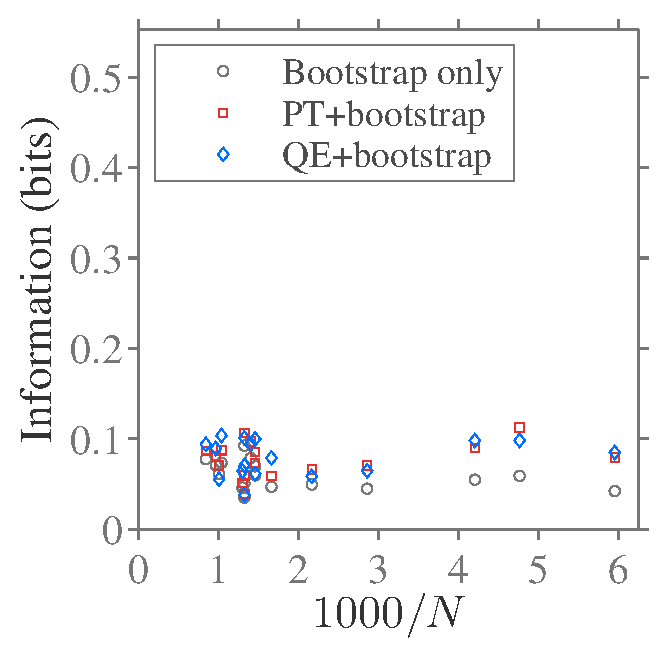
\includegraphics[scale=.45]{%
figs/info2/bias/ntrials_I_vs_invN_combindivpap_leg_blanco_v1_14chn_Gbalanced_1bins_of_527ms_btsp20.eps}}
    \hspace*{\fill}\hspace{.2cm}\hspace*{\fill}
    \subfloat[][\ac{M2} \ac{V1}.\label{fig:I_vs_invN_btsp_v1_jack}]{%
        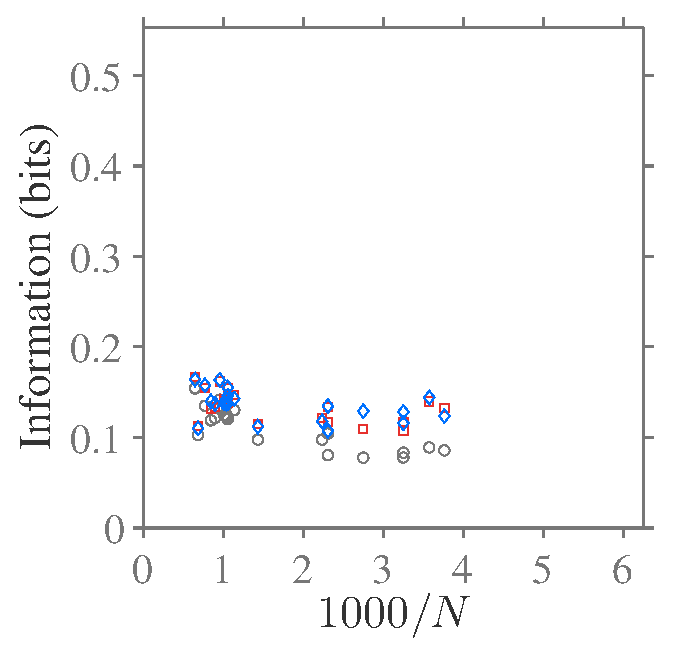
\includegraphics[scale=.45]{%
figs/info2/bias/ntrials_I_vs_invN_combindivpap_blanco_v4_25chn_Gbalanced_1bins_of_527ms_btsp20.eps}}
    \hspace*{\fill}
    \\
    \hspace*{\fill}
    \subfloat[][\ac{M1} \ac{V4}.\label{fig:I_vs_invN_btsp_v4_blanco}]{%
        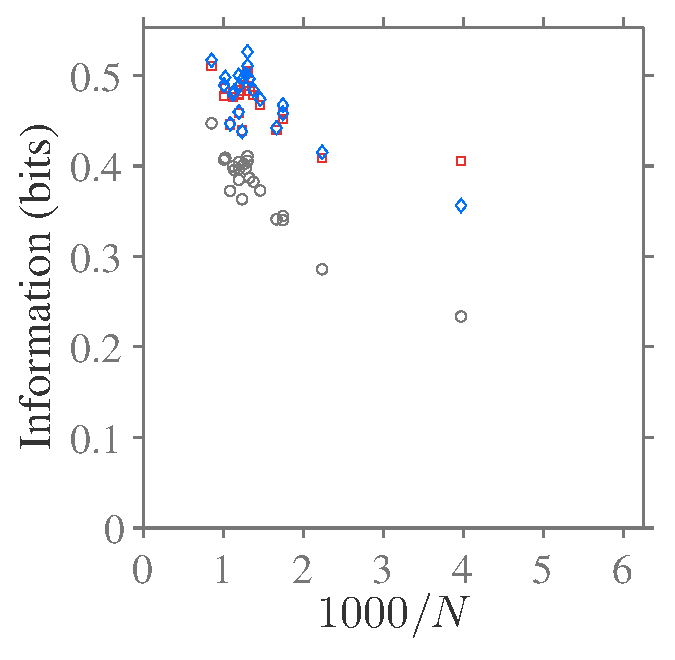
\includegraphics[scale=.45]{%
figs/info2/bias/ntrials_I_vs_invN_combindivpap_jack_v1_20chn_Gbalanced_1bins_of_527ms_btsp20.eps}}
    \hspace*{\fill}\hspace{.2cm}\hspace*{\fill}
    \subfloat[][\ac{M2} \ac{V4}.\label{fig:I_vs_invN_btsp_v4_jack}]{%
        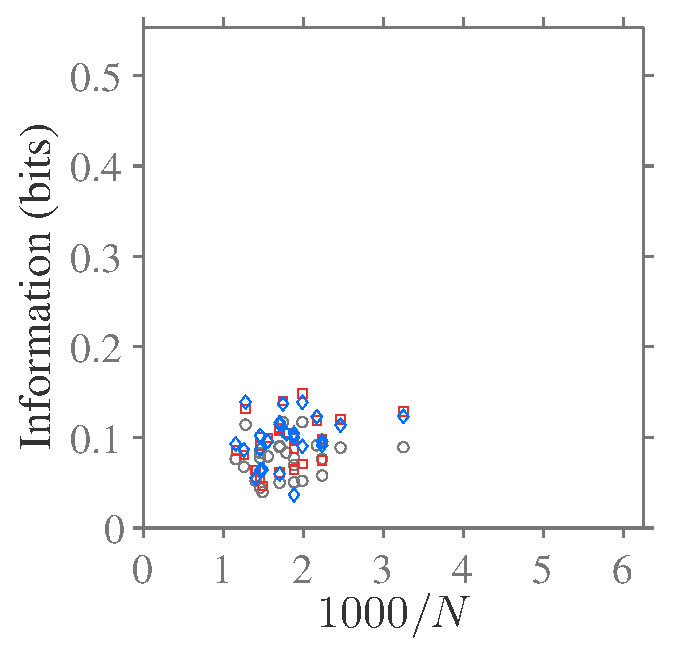
\includegraphics[scale=.45]{%
figs/info2/bias/ntrials_I_vs_invN_combindivpap_jack_v4_18chn_Gbalanced_1bins_of_527ms_btsp20.eps}}
    \hspace*{\fill}
    \caption{Distribution of measured information as a function of $\nicefrac{1}{N}$, where $N$ is the number of trials in the session.
Results are shown with bias correction either achieved solely from subtracting the information contained in response-shuffled copies of the data (grey circles), or by combining this with a better principled bias correction technique (\ac{PT}, red squares; \ac{QE}, blue diamonds).
Information was computed after using subsampling to address the stimulus class imbalance (see \autoref{sec:pl_class_imbalance}), and this is reflected in the value of $N$.
}
    \label{fig:I_vs_invN_btsp}
\end{figure}

We find that using bootstrapping for the bias correction does indeed overestimate the bias, resulting in a negative correlation between information and $\nicefrac{1}{N}$.
This effect is particularly dominant for the \ac{M1} \ac{V4} dataset (see \autoref{fig:I_vs_invN_btsp_v4_blanco}).

%------------------------------------
 \subsubsection{Grouping stimuli together}
 \label{sec:pl_bias_grouping}

During the experiment, the subject is tasked with determining whether the stimulus contrast is higher or lower than the \SI{30}{\percent} sample stimulus presented at the start of each trial.
As a consequence of this, the subject does not need to learn exactly what stimulus is on screen, only whether the stimulus is in the half above or below \SI{30}{\percent} contrast.
For instance, since the target output is the same for \SI{31}{\percent} and \SI{32}{\percent} contrast stimuli, there is no need for the subject to discriminate between them, but there is motivation for the subject to learn to discriminate between these and the \SI{29}{\percent} contrast stimulus.


\begin{figure}[htbp]
    \centering
    \hspace*{\fill}
    \subfloat[][\ac{M1} \ac{V1}.\label{fig:I_vs_invN_target-group_v1_blanco}]{%
        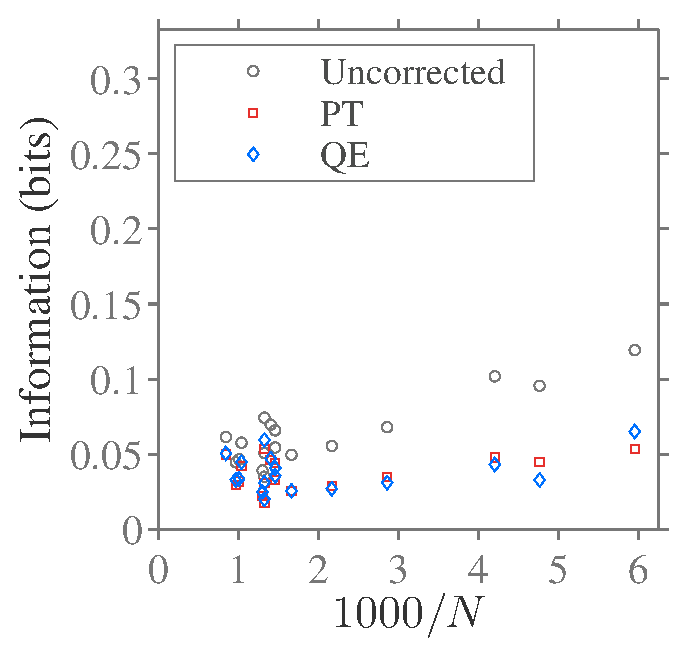
\includegraphics[scale=.45]{%
figs/info2/bias/ntrials_I_vs_invN_combindivpap_leg_blanco_v1_14chn_Gclass-group-balanced_1bins_of_527ms.eps}}
    \hspace*{\fill}\hspace{.2cm}\hspace*{\fill}
    \subfloat[][\ac{M2} \ac{V1}.\label{fig:I_vs_invN_target-group_v1_jack}]{%
        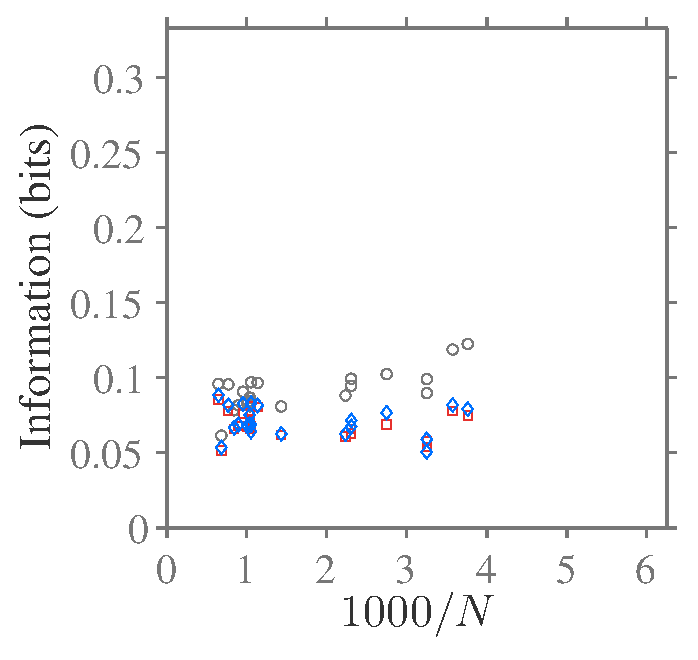
\includegraphics[scale=.45]{%
figs/info2/bias/ntrials_I_vs_invN_combindivpap_blanco_v4_25chn_Gclass-group-balanced_1bins_of_527ms.eps}}
    \hspace*{\fill}
    \\
    \hspace*{\fill}
    \subfloat[][\ac{M1} \ac{V4}.\label{fig:I_vs_invN_target-group_v4_blanco}]{%
        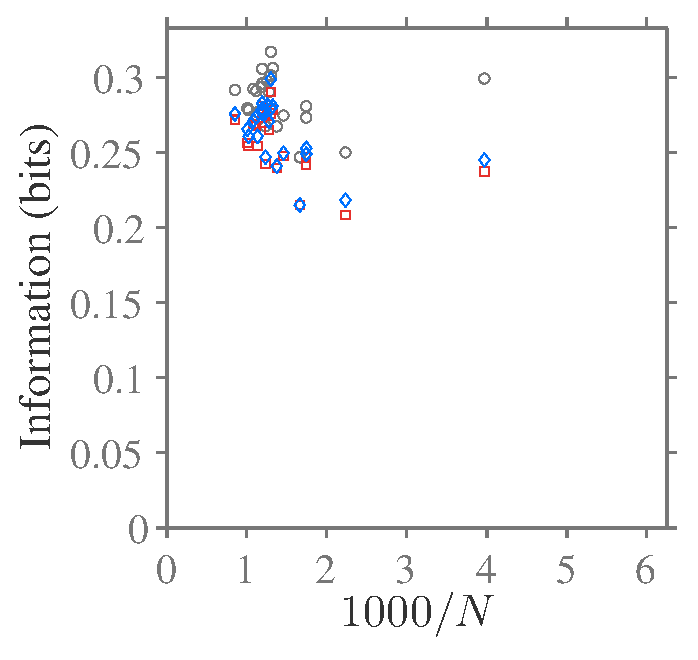
\includegraphics[scale=.45]{%
figs/info2/bias/ntrials_I_vs_invN_combindivpap_jack_v1_20chn_Gclass-group-balanced_1bins_of_527ms.eps}}
    \hspace*{\fill}\hspace{.2cm}\hspace*{\fill}
    \subfloat[][\ac{M2} \ac{V4}.\label{fig:I_vs_invN_target-group_v4_jack}]{%
        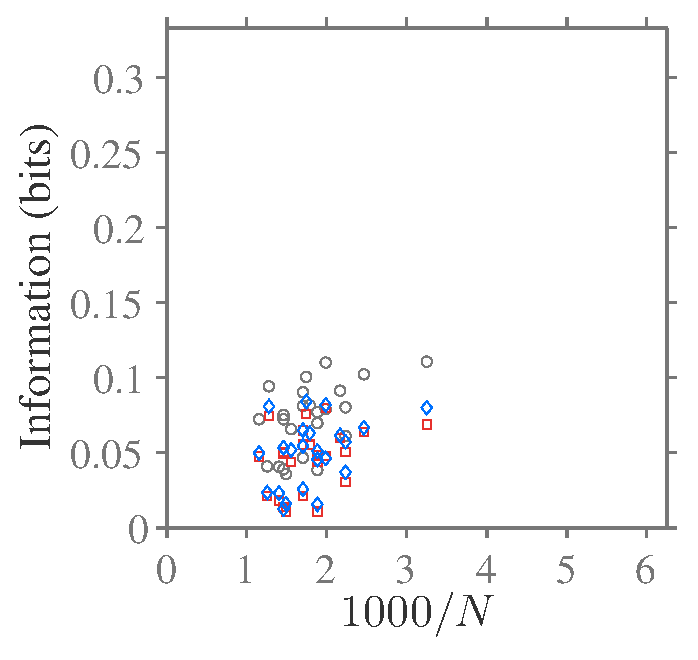
\includegraphics[scale=.45]{%
figs/info2/bias/ntrials_I_vs_invN_combindivpap_jack_v4_18chn_Gclass-group-balanced_1bins_of_527ms.eps}}
    \hspace*{\fill}
    \caption{Distribution of measured information as a function of $\nicefrac{1}{N}$, where $N$ is the number of trials in the session.
Results are shown both without correcting for the finite measurement bias (grey circles), using \ac{PT} bias correction (red squares), and using \ac{QE} bias correction (blue diamonds).
Information was computed after using subsampling to address the stimulus class imbalance (see \autoref{sec:pl_class_imbalance}), and this is reflected in the value of $N$.
}
    \label{fig:I_vs_invN_target-group}
\end{figure}

Grouping the stimuli together in this manner reduces the total amount of information which is measured (compare the $y$-axis scale bars of \autoref{fig:I_vs_invN_target-group} with \autoref{fig:I_vs_invN}).
The fraction of information encoded in the neural response which is task-specific is investigated in more detail in \autoref{sec:task-info}.
For now, we are only concerned with whether we can prevent differences in information estimation between sessions due to a shortage of trials per stimulus by grouping together the stimuli into two categories.

As anticipated, using only two stimulus classes to increase the number of trials per stimulus class greatly reduces the residual bias after \ac{PT} bias correction.
This is witnessed in the reduced correlation between estimated information and $\nicefrac{1}{N}$ seen in \autoref{fig:I_vs_invN_target-group}.

%------------------------------------
 \subsubsection{Trial-wise analysis}

We now consider what happens if we group together trials from multiple sessions into a single block and analyse them together.
Doing so allows us overcome the difference in bias between sessions, since the same number of trials would be used in each block and this can be set large enough to ensure we are in the correct domain for bias correction perform adequately.
There are typically no more than $25$ different firing rates for any single channel, so we grouped together $100$ trials of each stimulus condition.

Using this methodology, we focus on the subject's performance as a function of the number of trials which they have completed since the beginning of the experiment, irrespective of how many training sessions these trials are spread across.
Therefore, such a technique makes sense if we consider learning to occur during sessions and not to occur between them.
However, such a view is in contrast with the hypothesis that one of the important functions of sleep is to facilitate consolidation of memories and learning from during the day.
Should this be an important contributor towards perceptual learning, one would expect the breaks between sessions not to be irrelevant but to instead enable an increase in performance even without exposure to the training stimuli.


\begin{figure}[htbp]%
    \centering
    \hspace*{\fill}
    \subfloat[][\ac{M1} \ac{V1}.\label{fig:info_trial_1x527_balanced_v1_blanco}]{%
        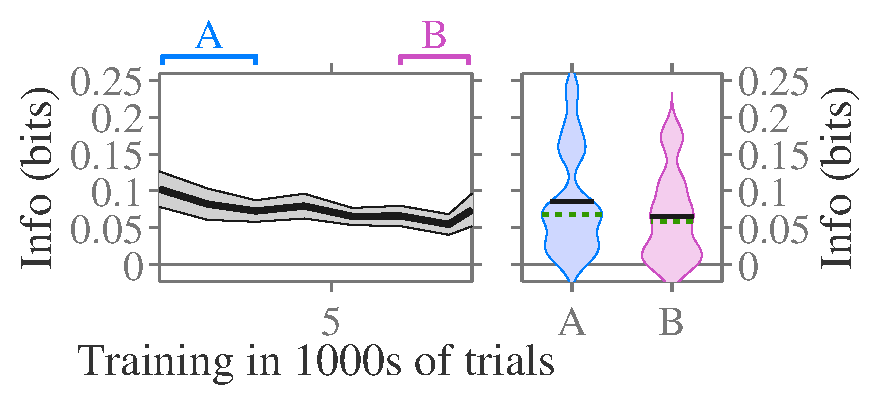
\includegraphics[scale=.45]{%
figs/info2/bias/I_trialwise_blanco_v1_chmean14_s343-354,355.1,355.2,356-359_tp4_1bins_of_527ms_dr_pt_oc0_Gbalanced_test_tc5-5-20,22-3-28,32,35-5-50,60,90_nt1400_ts1400_rmvet2_rmvms2_imscn_clhot.eps}}
    \hspace*{\fill}\hspace{.2cm}\hspace*{\fill}
    \subfloat[][\ac{M2} \ac{V1}.\label{fig:info_trial_1x527_balanced_v1_jack}]{%
        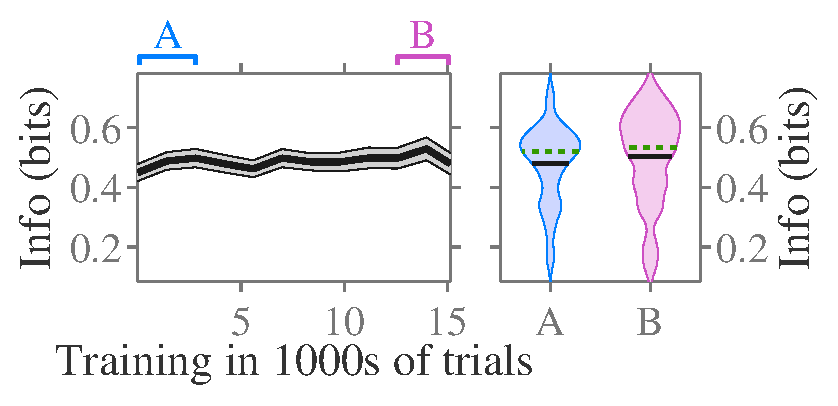
\includegraphics[scale=.45]{%
figs/info2/bias/I_trialwise_jack_v1_chmean20_s51-72_tp4_1bins_of_527ms_dr_pt_oc0_Gbalanced_test_tc5-5-20,22-3-28,32,35-5-50,60,90_nt1400_ts1400_rmvet2_rmvms2_imscn_clhot.eps}}
    \hspace*{\fill}
    \\
    \hspace*{\fill}
    \subfloat[][\ac{M1} \ac{V4}.\label{fig:info_trial_1x527_balanced_v4_blanco}]{%
        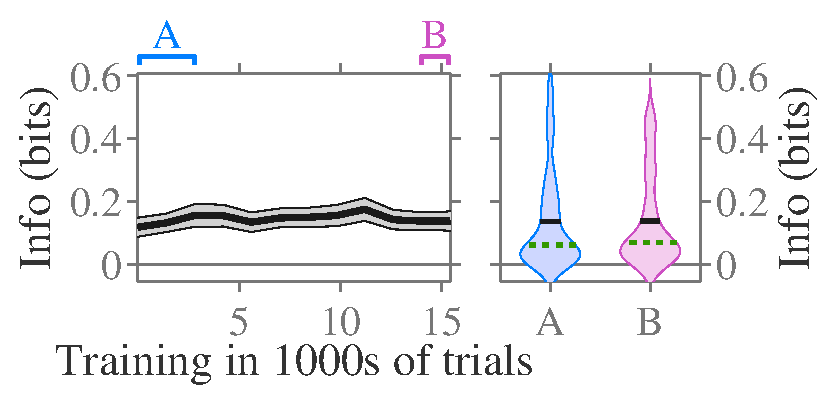
\includegraphics[scale=.45]{%
figs/info2/bias/I_trialwise_blanco_v4_chmean25_s307,308,311,313,314,317,318,320,321,329-341_tp4_1bins_of_527ms_dr_pt_oc0_Gbalanced_test_tc10-5-25,27-29,31-33,35,40-10-60_nt1400_ts1400_rmvet2_rmvms2_imscn_clhot.eps}}
    \hspace*{\fill}\hspace{.2cm}\hspace*{\fill}
    \subfloat[][\ac{M2} \ac{V4}.\label{fig:info_trial_1x527_balanced_v4_jack}]{%
        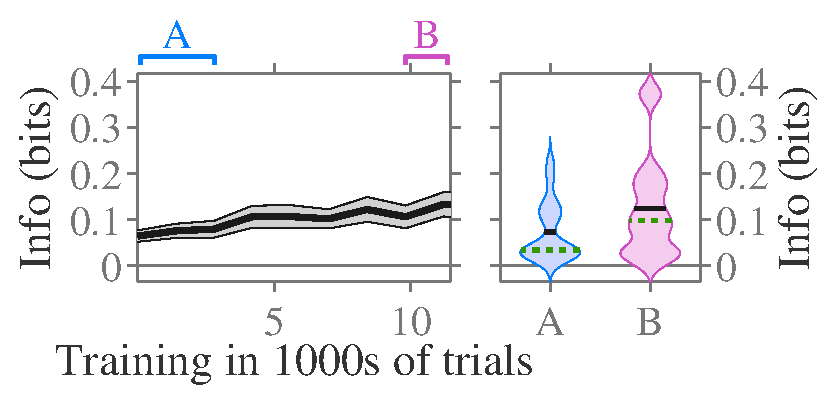
\includegraphics[scale=.45]{%
figs/info2/bias/I_trialwise_jack_v4_chmean18_s24,25,27-38,40-49_tp4_1bins_of_527ms_dr_pt_oc0_Gbalanced_test_tc10-5-25,27-29,31-33,35,40-10-60_nt1400_ts1400_rmvet2_rmvms2_imscn_clhot.eps}}
    \hspace*{\fill}
    \caption{Information about the test stimulus contained in the firing rate during test presentation and its progression over training sessions, estimated across blocks of $100$ consecutive trials of each stimulus class taken by merging consecutive sessions together to accumulate sufficiently many trials.
Main panels: the average over channels (\protect\subref{fig:info_trial_1x527_balanced_v1_blanco}~$14$ channels, \protect\subref{fig:info_trial_1x527_balanced_v1_jack}~$20$ channels, \protect\subref{fig:info_trial_1x527_balanced_v4_blanco}~$25$ channels, \protect\subref{fig:info_trial_1x527_balanced_v4_jack}~$18$ channels) with standard error over channels indicated by the shaded region.
Right hand panels: distribution over channels of the information contained in the first three blocks of $1400$ trials (\zonename{A}) versus last three blocks (\zonename{B}), with mean (solid black line) and median (dashed green line) over channels indicated.
The violin plot shows a Gaussian kernel density, using a bandwidth determined as described in \autoref{sec:info-methods}.
The \ac{PT} bias correction method was used, without further correction to the residual bias.
The stimulus class imbalance was address on a session-by-session basis by subsampling as described previously (\autoref{sec:pl_class_imbalance}) before merging sessions together.
}
    \label{fig:info_trial_1x527_balanced}
\end{figure}


Since we performed the spike extraction such that the spontaneous firing rate is held constant across sessions for each channel, the firing rate during stimulus presentation is comparable between sessions.
This means it is plausible that, when decoding the information, the extracted firing rate corresponding to the stimuli could be similar across consecutive sessions.

We find that grouping trials together in this way smooths out the problems with inter-session changes in residual bias on the information estimate.
But because of both changes in neural connectivity and small movement in the electrode contacts between sessions, the neural code is not guaranteed to be the same between sessions.
Indeed, we observed a peak in the estimated information corresponding to longer sessions where the trial sample size is smaller than or a similar size to the number of trials grouped together in each block.
For this reason, it is prudent not to proceed with such a methodology.


%------------------------------------------------------------------------------
\subsection{Task-pertinent and nonpertinent information}
% \subsection{Comparing information about the stimulus with task-relevant information}
\label{sec:task-info}

So far, we have been computing the amount of information in the neural response (more specifically, the firing rate over the stimulus presentation period) about the identity of the presented stimulus.
Computing the mutual information between these two tells us how much information we gain about which stimulus was presented when we are told how many spikes were detected with a given electrode contact.
However, the object the subject is tasked with is more specific --- to identify whether the presented stimulus has a contrast higher or lower than the pedestal contrast.
To achieve this goal, it is not necessary to distinguish exactly which stimulus was presented.

We can separate the information given by the neural response into two parts: task-pertinent and task-nonpertinent information.
The task-pertinent information helps us tell whether the stimulus was in the half above or below the pedestal contrast of \SI{30}{\percent}.
However we also gain information about exactly which stimuli within the upper and lower half of the set of contrasts is more likely to have been presented.
Although this information helps us distinguish which stimulus was presented (and hence presumably helps the subject perceive the stimuli more accurately), it is not pertinent to the subject's task.

For instance, any information which helps us discriminate between whether a \SI{29}{\percent} or \SI{31}{\percent} contrast stimulus was more likely to have been presented is pertinent to the task.
Whereas if we gain information about the stimulus which updates the probability of it having a \SI{28}{\percent} versus a \SI{29}{\percent} contrast without changing the probability that it was one of \SI{28}{\percent} or \SI{29}{\percent} contrast, this is not pertinent to the task.


\subsubsection{Methods}
\label{sec:task-info-methods}

First, we computed the total information contained in the neural response as before, using the total spikes recorded by a single channel over \SI{527}{\milli\second} of stimulus presentation as the response on each trial.
The finite sampling bias on the estimated information was corrected for using the \ac{PT} method, and further residual bias removed using bootstrapping (see \autoref{sec:pl_bootstrapping}).
Stimulus class imbalance was corrected for using subsampling, as described in \autoref{sec:pl_class_imbalance}.

The amount of task-pertinent information contained in the response was estimated by shuffling the stimulus labels against the responses, whilst preserving which side of \SI{30}{\percent} contrast the stimulus label was on.
This destroys any information about the stimulus beyond that pertinent to the task --- choosing whether the stimulus was above or below \SI{30}{\percent} contrast --- but maintains the number of class labels and samples per class.
Consequently, the bias on the information will be similar to that when computing the total information, and the results will be more directly comparable\footnote{However, the bias will not be the same for the two information values because after shuffling the range of possible values for the response will have increased. Consequently, it is still necessary to do individual bias correction with \ac{PT} and bootstrapping on each of the information computations.}.
We repeated this with $20$ permutations, each with their own set of $20$ bootstraps, and took the average across them.
The amount of task-nonpertinent information was estimated by subtracting the task-pertinent information (found with shuffling) from the total information (found without shuffling).

To compute the proportion of information encapsulated within the response which was pertinent to the task, we divided the estimated task-pertinent information by the total information (after correcting for the bias on each estimate).
To prevent channels whose responses contain negligible information about the stimulus contaminating the results with anomalously large (or small) outliers after the division, we excluded any channels whose total information was less than $1.5$ times the standard deviation across the bootstrapped information values.
Additionally, the proportional information reported for each channel was capped at $0$ and $1$ taking the average across channels.

To quantify the change over time, we again compared the information averaged over the first three sessions (\zonename{A}) with the information over the last three sessions (\zonename{B}).
For the relative information, only channels which had a significant amount of total information (exceeding $1.5$ times the standard deviation over bootstraps) for both \zonename{A} and \zonename{B} were included.
This step was included to ensure \zonename{A} and \zonename{B} were directly comparable; a paired $t$-test was used to compare the information at \zonename{A} with \zonename{B}.

Similarly, we considered the amount of information about the stimulus contained in the behavioural response of the animal, which was a saccade to one of two targets, indicating whether the subject believed the contrast to be higher or lower than \SI{30}{\percent} (two forced-choice).
The same procedure was used to decomposed the the total information in this response into task-pertinent and nonpertinent components, and find the proportion of the information which was task-pertinent.

Although it is only a binary response (a choice of one of two saccade targets), it is still possible for the behavioural response to encode both task-pertinent and task-nonpertinent information.
For instance, let us assume that the subject completes the task at a rate higher than chance.
Then, a behavioural response of ``\textit{test contrast is lower}'' tells us a contrast in the lower half was more likely to have been presented, providing task-pertinent information.
Additionally, since contrasts further from the \SI{30}{\percent} threshold are easier for the subject, we can empirically observe that a response of ``\textit{test contrast is lower}'' is more likely to be elicited if the contrast was further below the threshold than if it was close to the threshold\footnote{This trivially follows using Bayes' rule}.
This difference in relative likelihood supplies us with additional, task-nonpertinent, information about which stimulus was presented.


\subsubsection{\acs{V1} Results}

We separated the total information about the stimulus contained in the neural response into task-pertinent and task-nonpertinent components as described in \autoref{sec:task-info-methods}.
For \ac{M1}, there was a non-significant decrease in the total information, task-pertinent information, and the task-nonpertinent information between \zonename{A} and \zonename{B} (paired Student's $t$-test; $p=0.20$, $p=0.38$, and $p=0.13$ respectively), as shown in \autoref{fig:info_taskpertinent_v1_ch_blanco}.
Correspondingly, there was no significant change in the fraction of the total information which was task-pertinent either ($p=0.60$; see \autoref{fig:info_taskpertinent_rel_v1_ch_blanco}).

For \ac{M2}, there was a small, non-significant, decrease in the task-nonpertinent information between \zonename{A} and \zonename{B} (\SI{-0.010\pm0.007}{bits}, $p=0.16$), but there was a significant increase in the task-pertinent information (\SI{+0.060\pm0.011}{bits}, $p=0.00002$; see \autoref{fig:info_taskpertinent_v1_ch_jack}).
Together, these give a combined increase in the total information of \SI{+0.050\pm0.015}{bits} ($p=0.004$).
Since the task-nonpertinent information is stable while the task-pertinent information increases with training, the proportion of encoded information which is task-pertinent increases by \SI{+7.0\pm1.3}{\percent} ($p=0.00004$), as shown in \autoref{fig:info_taskpertinent_rel_v1_ch_jack}.

% blanco v1 1x527.00ms
% dr pt
% For Total Info (bits)
% n=14  h=0.000000  p=0.205484=2.054842e-01   delta = -0.026854+/-0.020149 = -29.290339%+/-22.139211%
% For Task-pertinent Info (bits)
% n=14  h=0.000000  p=0.375025=3.750246e-01   delta = -0.010713+/-0.011662 = -25.593377%+/-27.886183%
% For Task-nonpertinent Info (bits)
% n=14  h=0.000000  p=0.133354=1.333535e-01   delta = -0.016142+/-0.010081 = -32.396084%+/-20.293906%
% selected bw  :  bandwidth=0.011217
%
% For Task-pertinent Info (%)
% n=4  h=0.000000  p=0.596176=5.961759e-01   delta = +4.414025+/-7.470531 = +10.618742%+/-533.852117%
% For Task-nonpertinent Info (%)
% n=4  h=0.000000  p=0.596176=5.961759e-01   delta = -4.414025+/-7.470531 = -7.554155%+/-533.702687%
% selected bw  :  bandwidth=2.813857
%
%
% jack v1 1x527.00ms
% dr pt
% For Total Info (bits)
% n=20  h=1.000000  p=0.003762=3.761940e-03   delta = +0.049989+/-0.015146 = +11.458962%+/-4.411886%
% For Task-pertinent Info (bits)
% n=20  h=1.000000  p=0.000020=2.022440e-05   delta = +0.060332+/-0.010732 = +28.392210%+/-5.205318%
% For Task-nonpertinent Info (bits)
% n=20  h=0.000000  p=0.162219=1.622189e-01   delta = -0.010343+/-0.007113 = -4.622742%+/-3.554708%
% selected bw  :  bandwidth=0.015976
%
% For Task-pertinent Info (%)
% n=20  h=1.000000  p=0.000036=3.596357e-05   delta = +7.049025+/-1.315612 = +14.317851%+/-97.552405%
% For Task-nonpertinent Info (%)
% n=20  h=1.000000  p=0.000036=3.596357e-05   delta = -7.049025+/-1.315612 = -13.884894%+/-97.550225%
% selected bw  :  bandwidth=1.236527

\begin{figure}[htbp]%
    \centering
    \hspace*{\fill}
    \subfloat[][\ac{M1} \ac{V1} Information.\label{fig:info_taskpertinent_v1_ch_blanco}]{%
        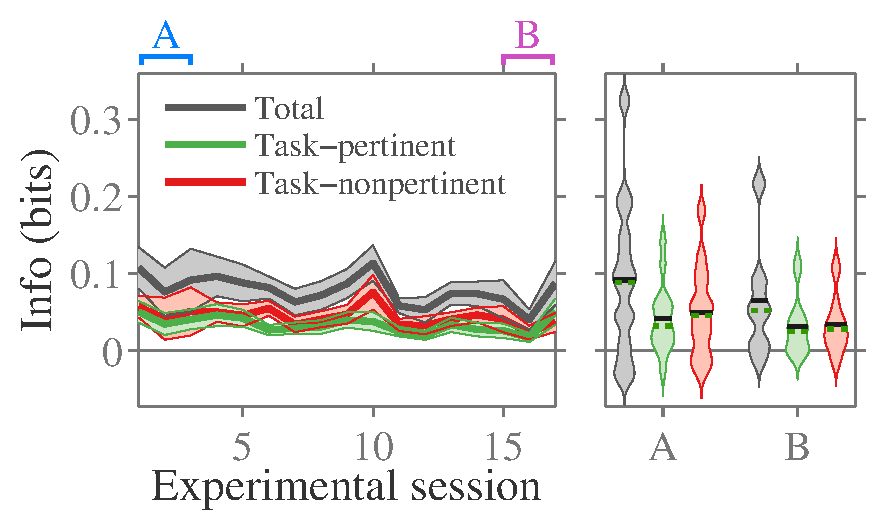
\includegraphics[scale=.45]{%
figs/info2/task-pertinent/I_sessionwise_blanco_v1_chmean14_s343-359_oc0_Gclass-shuffled-balanced_1bins_of_527ms_dr_pt_btsp20_rmvet2_rmvms2_info_leg.eps}}
    \hspace*{\fill}\hspace{.2cm}\hspace*{\fill}
    \subfloat[][\ac{M2} \ac{V1} Information.\label{fig:info_taskpertinent_v1_ch_jack}]{%
        \includegraphics[scale=.45]{%
figs/info2/task-pertinent/I_sessionwise_jack_v1_chmean20_s51-72_oc0_Gclass-shuffled-balanced_1bins_of_527ms_dr_pt_btsp20_rmvet2_rmvms2_info.eps}}
    \hspace*{\fill}
    \\
    \hspace*{\fill}
    \subfloat[][\ac{M1} \ac{V1} Relative information.\label{fig:info_taskpertinent_rel_v1_ch_blanco}]{%
        \includegraphics[scale=.45]{%
figs/info2/task-pertinent/I_sessionwise_blanco_v1_chmean14_s343-359_oc0_Gclass-shuffled-balanced_1bins_of_527ms_dr_pt_btsp20_rmvet2_rmvms2_relative-info.eps}}
    \hspace*{\fill}\hspace{.2cm}\hspace*{\fill}
    \subfloat[][\ac{M2} \ac{V1} Relative information.\label{fig:info_taskpertinent_rel_v1_ch_jack}]{%
        \includegraphics[scale=.45]{%
figs/info2/task-pertinent/I_sessionwise_jack_v1_chmean20_s51-72_oc0_Gclass-shuffled-balanced_1bins_of_527ms_dr_pt_btsp20_rmvet2_rmvms2_relative-info.eps}}
    \hspace*{\fill}
    \caption{Breakdown of task-pertinent and nonpertinent information contained in \ac{V1} recording channels.
In \protect\subref{fig:info_taskpertinent_v1_ch_blanco} and \protect\subref{fig:info_taskpertinent_v1_ch_jack}, the total information about the stimulus (grey), task-pertinent information (green), and task-nonpertinent (red) contained in each of $14$ and $20$ channels respectively.
In \protect\subref{fig:info_taskpertinent_rel_v1_ch_blanco} and \protect\subref{fig:info_taskpertinent_rel_v1_ch_jack}, the relative information about the stimulus which is task-pertinent (green) and task-nonpertinent (red) contained in channels with a significant amount of total information ($4$ and $20$ respectively).
Main panels: across training sessions, the average information over channels, with standard error over channels indicated by the shaded region.
Right hand panels: distribution over channels of the information (or relative information) in the first three sessions (\zonename{A}) versus last three sessions (\zonename{B}), with mean (solid black line) and median (dashed green line) over channels indicated.
The violin plot shows a Gaussian kernel density, using a bandwidth determined as described in \autoref{sec:info-methods}.
The \ac{PT} bias correction method was used, with the residual bias further reduced using bootstrapping (see \autoref{sec:pl_bootstrapping}).
The stimulus class imbalance was corrected using subsampling, as described in \autoref{sec:pl_class_imbalance}.
    \label{fig:info_taskpertinent_v1_ch}
}
\end{figure}


Over the same period of training, we examined the decomposition of the information contained in the behavioural response of the experimental subject.
Similar trends were found for \ac{M1} and \ac{M2}.
There was a vast increase in the amount of task-pertinent information between \zonename{A} and \zonename{B} of \SI{+0.32}{bits} and \SI{+0.34}{bits} respectively, which more than tripled the amount of task-pertinent information given in the subject's response between the beginning and end of the experiment.
The task-nonpertinent information in the response increased by a modest \SI{+0.06}{bits} and \SI{+0.03}{bits} respectively, which is a relative increase of \SI{71}{\percent} and \SI{32}{\percent} from \zonename{A} to \zonename{B}.
Collectively, this meant the proportion of information which was task-pertinent increased from near \SI{60}{\percent} to near \SI{80}{\percent} for both subjects.

% Behavioural info for blanco v1
% For Total Info (bits)
% n=1  h=NaN  p=NaN=NaN   delta = +0.381066+/-0.000000 = +172.797622%+/-0.000000%
% For Task-pertinent Info (bits)
% n=1  h=NaN  p=NaN=NaN   delta = +0.323136+/-0.000000 = +230.776949%+/-0.000000%
% For Task-nonpertinent Info (bits)
% n=1  h=NaN  p=NaN=NaN   delta = +0.057930+/-0.000000 = +71.956869%+/-0.000000%
% For Task-pertinent Info (%)
% n=1  h=NaN  p=NaN=NaN   delta = +13.494701+/-0.000000 = +21.253604%+/-0.000000%
% For Task-nonpertinent Info (%)
% n=1  h=NaN  p=NaN=NaN   delta = -13.494701+/-0.000000 = -36.965408%+/-0.000000%
%
% Behavioural info for jack v1
% For Total Info (bits)
% n=1  h=NaN  p=NaN=NaN   delta = +0.366698+/-0.000000 = +139.268115%+/-0.000000%
% For Task-pertinent Info (bits)
% n=1  h=NaN  p=NaN=NaN   delta = +0.335353+/-0.000000 = +201.184738%+/-0.000000%
% For Task-nonpertinent Info (bits)
% n=1  h=NaN  p=NaN=NaN   delta = +0.031345+/-0.000000 = +32.443197%+/-0.000000%
% For Task-pertinent Info (%)
% n=1  h=NaN  p=NaN=NaN   delta = +16.382229+/-0.000000 = +25.877507%+/-0.000000%
% For Task-nonpertinent Info (%)
% n=1  h=NaN  p=NaN=NaN   delta = -16.382229+/-0.000000 = -44.646533%+/-0.000000%

\begin{figure}[htbp]%
    \centering
    \hspace*{\fill}
    \subfloat[][\ac{M1} \ac{V1} Information.\label{fig:info_taskpertinent_v1_behav_blanco}]{%
        \includegraphics[scale=.45]{%
figs/info2/task-pertinent/I_behav_blanco_v1_s343-359_Gclass-shuffled-balanced_dr_pt_btsp20_rmvet2_info.eps}}
    \hspace*{\fill}\hspace{.2cm}\hspace*{\fill}
    \subfloat[][\ac{M2} \ac{V1} Information.\label{fig:info_taskpertinent_v1_behav_jack}]{%
        \includegraphics[scale=.45]{%
figs/info2/task-pertinent/I_behav_jack_v1_s51-72_Gclass-shuffled-balanced_dr_pt_btsp20_rmvet2_info.eps}}
    \hspace*{\fill}
    \\
    \hspace*{\fill}
    \subfloat[][\ac{M1} \ac{V1} Relative information.\label{fig:info_taskpertinent_rel_v1_behav_blanco}]{%
        \includegraphics[scale=.45]{%
figs/info2/task-pertinent/I_behav_blanco_v1_s343-359_Gclass-shuffled-balanced_dr_pt_btsp20_rmvet2_relative-info.eps}}
    \hspace*{\fill}\hspace{.2cm}\hspace*{\fill}
    \subfloat[][\ac{M2} \ac{V1} Relative information.\label{fig:info_taskpertinent_rel_v1_behav_jack}]{%
        \includegraphics[scale=.45]{%
figs/info2/task-pertinent/I_behav_jack_v1_s51-72_Gclass-shuffled-balanced_dr_pt_btsp20_rmvet2_relative-info.eps}}
    \hspace*{\fill}
    \caption{Breakdown of task-pertinent and nonpertinent information contained in behavioural responses during \ac{V1} recording.
In \protect\subref{fig:info_taskpertinent_v1_behav_blanco} and \protect\subref{fig:info_taskpertinent_v1_behav_jack}, the total information about the stimulus (grey), task-pertinent information (green), and task-nonpertinent (red) contained the behavioural response on each trial.
In \protect\subref{fig:info_taskpertinent_rel_v1_behav_blanco} and \protect\subref{fig:info_taskpertinent_rel_v1_behav_jack}, the relative information about the stimulus which is task-pertinent (green) and task-nonpertinent (red).
The \ac{PT} bias correction method was used, with the residual bias further reduced using bootstrapping (see \autoref{sec:pl_bootstrapping}).
The stimulus class imbalance was corrected using subsampling, as described in \autoref{sec:pl_class_imbalance}.
    \label{fig:info_taskpertinent_v1_behav}
}
\end{figure}


\subsubsection{\acs{V4} Results}

For \ac{M1}, we found no significant change in the total, task-pertinent, or task-nonpertinent information about the stimulus encoded in \ac{V4} channels ($p=0.48$, $p=0.19$, and $p=0.94$ respectively; see \autoref{fig:info_taskpertinent_v4_ch_blanco}).
There was a small, but non-significant, increase of \SI{+0.014\pm0.010}{bits} in the average task-pertinent information between \zonename{A} and \zonename{B}.
Correspondingly, there was no significant change in the fraction of information which was task-pertinent either ($p=0.61$; see \autoref{fig:info_taskpertinent_rel_v4_ch_blanco}).

On the other hand, for \ac{M2} there was a significant ($p=0.0005$) increase in task-pertinent information from \zonename{A} to \zonename{B}, increasing by \SI{+0.054\pm0.013}{bits}, which is approximately $5$ times its initial value.
Meanwhile, the amount of task-nonpertinent information did not notably change (\SI{+0.008\pm0.008}{bits}, $p=0.32$).
Together, these effects accumulatively produced an significant increase in total information of \SI{+0.062\pm0.018}{bits} ($p=0.003$).
As a consequence of this, the proportion of information which is task-pertinent increased from under \SI{20}{\percent} to around \SI{50}{\percent}, with a swing from \zonename{A} to \zonename{B} of \SI{+33\pm3}{\percent} ($p=0.00005$).

Most information is initially not pertinent to the task, which may relate to most channels initially being inhibited by sample stimulus, as described in \autoref{sec:pl_dprime_v4} (\autoref{fig:dprime_v4_jack}).
The largest increase in task-pertinent information occurs on the 5th experimental session.
This corresponds to a session where several channels changed from stimulus-inhibited (negative $d'$) to stimulus-excited (positive $d'$).

% blanco v4 1x527.00ms
% dr pt
% For Total Info (bits)
% n=25  h=0.000000  p=0.480089=4.800887e-01   delta = +0.014921+/-0.020800 = +12.563164%+/-17.729269%
% For Task-pertinent Info (bits)
% n=25  h=0.000000  p=0.192543=1.925430e-01   delta = +0.014002+/-0.010443 = +26.745305%+/-19.984138%
% For Task-nonpertinent Info (bits)
% n=25  h=0.000000  p=0.941701=9.417010e-01   delta = +0.000919+/-0.012434 = +1.383585%+/-18.794865%
% selected bw  :  bandwidth=0.016494
%
% For Task-pertinent Info (%)
% n=13  h=0.000000  p=0.613049=6.130492e-01   delta = -2.717323+/-5.233468 = -5.561730%+/-601.681813%
% For Task-nonpertinent Info (%)
% n=13  h=0.000000  p=0.613049=6.130492e-01   delta = +2.717323+/-5.233468 = +5.313240%+/-601.673483%
% selected bw  :  bandwidth=3.203598
%
% jack v4 1x527.00ms
% dr pt
% For Total Info (bits)
% n=18  h=1.000000  p=0.002821=2.821313e-03   delta = +0.062224+/-0.017844 = +108.817777%+/-31.227202%
% For Task-pertinent Info (bits)
% n=18  h=1.000000  p=0.000527=5.272562e-04   delta = +0.054160+/-0.012710 = +505.870407%+/-118.716410%
% For Task-nonpertinent Info (bits)
% n=18  h=0.000000  p=0.321069=3.210688e-01   delta = +0.008065+/-0.007890 = +17.352317%+/-17.000845%
% selected bw  :  bandwidth=0.004437
%
% For Task-pertinent Info (%)
% n=7  h=1.000000  p=0.000051=5.059743e-05   delta = +33.408297+/-3.262665 = +136.706215%+/-360.592804%
% For Task-nonpertinent Info (%)
% n=7  h=1.000000  p=0.000051=5.059743e-05   delta = -33.408297+/-3.262665 = -44.213106%+/-360.371435%
% selected bw  :  bandwidth=2.699929

\begin{figure}[htbp]%
    \centering
    \hspace*{\fill}
    \subfloat[][\ac{M1} \ac{V4} Information.\label{fig:info_taskpertinent_v4_ch_blanco}]{%
        \includegraphics[scale=.45]{%
figs/info2/task-pertinent/I_sessionwise_blanco_v4_chmean25_s307,308,311,313,314,317,318,320,321,329-341_oc0_Gclass-shuffled-balanced_1bins_of_527ms_dr_pt_btsp20_rmvet2_rmvms2_info_leg.eps}}
    \hspace*{\fill}\hspace{.2cm}\hspace*{\fill}
    \subfloat[][\ac{M2} \ac{V4} Information.\label{fig:info_taskpertinent_v4_ch_jack}]{%
        \includegraphics[scale=.45]{%
figs/info2/task-pertinent/I_sessionwise_jack_v4_chmean18_s24,25,27-38,40-49_oc0_Gclass-shuffled-balanced_1bins_of_527ms_dr_pt_btsp20_rmvet2_rmvms2_info.eps}}
    \hspace*{\fill}
    \\
    \hspace*{\fill}
    \subfloat[][\ac{M1} \ac{V4} Relative information.\label{fig:info_taskpertinent_rel_v4_ch_blanco}]{%
        \includegraphics[scale=.45]{%
figs/info2/task-pertinent/I_sessionwise_blanco_v4_chmean25_s307,308,311,313,314,317,318,320,321,329-341_oc0_Gclass-shuffled-balanced_1bins_of_527ms_dr_pt_btsp20_rmvet2_rmvms2_relative-info_leg.eps}}
    \hspace*{\fill}\hspace{.2cm}\hspace*{\fill}
    \subfloat[][\ac{M2} \ac{V4} Relative information.\label{fig:info_taskpertinent_rel_v4_ch_jack}]{%
        \includegraphics[scale=.45]{%
figs/info2/task-pertinent/I_sessionwise_jack_v4_chmean18_s24,25,27-38,40-49_oc0_Gclass-shuffled-balanced_1bins_of_527ms_dr_pt_btsp20_rmvet2_rmvms2_relative-info.eps}}
    \hspace*{\fill}
    \caption{Breakdown of task-pertinent and nonpertinent information contained in \ac{V4} recording channels.
In \protect\subref{fig:info_taskpertinent_v4_ch_blanco} and \protect\subref{fig:info_taskpertinent_v4_ch_jack}, the total information about the stimulus (grey), task-pertinent information (green), and task-nonpertinent (red) contained in each of $25$ and $18$ channels respectively.
In \protect\subref{fig:info_taskpertinent_rel_v4_ch_blanco} and \protect\subref{fig:info_taskpertinent_rel_v4_ch_jack}, the relative information about the stimulus which is task-pertinent (green) and task-nonpertinent (red) contained in channels with a significant amount of total information ($13$ and $7$ respectively).
Main panels: across training sessions, the average information over channels, with standard error over channels indicated by the shaded region.
Right hand panels: distribution over channels of the information (or relative information) in the first three sessions (\zonename{A}) versus last three sessions (\zonename{B}), with mean (solid black line) and median (dashed green line) over channels indicated.
The violin plot shows a Gaussian kernel density, using a bandwidth determined as described in \autoref{sec:info-methods}.
The \ac{PT} bias correction method was used, with the residual bias further reduced using bootstrapping (see \autoref{sec:pl_bootstrapping}).
The stimulus class imbalance was corrected using subsampling, as described in \autoref{sec:pl_class_imbalance}.
    \label{fig:info_taskpertinent_v4_ch}
}
\end{figure}


The behavioural information for \ac{V4} training sessions shows a similar trend to the behavioural information during \ac{V1} training sessions.
Namely, there is a larger increase in task-pertinent information and a smaller increase in task-nonpertinent information.

For \ac{M1}, the subject began training with a decent initial performance, and correspondingly a decent amount of task-pertinent information is given by the behavioural response, as shown in \autoref{fig:info_taskpertinent_v4_behav_blanco}.
Indeed, for \ac{M1} around \SI{75}{\percent} of the information contained in the behavioural response is task-pertinent at the beginning of training, and this percentage does not notably change throughout training (see \autoref{fig:info_taskpertinent_rel_v4_behav_blanco}).
The total information encoded in the neural response does increase with training, but the most of this arising from an increase in task-pertinent information (\SI{+0.128}{bits}) as opposed to nonpertinent information (\SI{+0.034}{bits}).

Compared to \ac{M1}, subject \ac{M2} began training with very poor performance on the task.
Correspondingly, the behavioural response initially provides less information about which stimulus was presented (see \autoref{fig:info_taskpertinent_v4_behav_jack}) --- and over \SI{80}{\percent} of that is not pertinent to the task (see \autoref{fig:info_taskpertinent_rel_v4_behav_jack}).
The amount of task-pertinent information given by the behavioural response increases by \SI{0.238}{bits} from \zonename{A} to \zonename{B} (a 26-fold increase), whilst the task-nonpertinent information doubles, only increasing by \SI{0.057}{bits}.
Consequently, there is a massive swing of \SI{+54}{\percent} in the fraction of information encoded in the behavioural response which is task-pertinent.

% Behavioural info for blanco v4
% For Total Info (bits)
% n=1  h=NaN  p=NaN=NaN   delta = +0.162043+/-0.000000 = +44.813597%+/-0.000000%
% For Task-pertinent Info (bits)
% n=1  h=NaN  p=NaN=NaN   delta = +0.127796+/-0.000000 = +47.636289%+/-0.000000%
% For Task-nonpertinent Info (bits)
% n=1  h=NaN  p=NaN=NaN   delta = +0.034247+/-0.000000 = +36.698947%+/-0.000000%
% For Task-pertinent Info (%)
% n=1  h=NaN  p=NaN=NaN   delta = +1.446146+/-0.000000 = +1.949190%+/-0.000000%
% For Task-nonpertinent Info (%)
% n=1  h=NaN  p=NaN=NaN   delta = -1.446146+/-0.000000 = -5.603514%+/-0.000000%
%
% Behavioural info for jack v4
% For Total Info (bits)
% n=1  h=NaN  p=NaN=NaN   delta = +0.294209+/-0.000000 = +485.223076%+/-0.000000%
% For Task-pertinent Info (bits)
% n=1  h=NaN  p=NaN=NaN   delta = +0.237539+/-0.000000 = +2537.475948%+/-0.000000%
% For Task-nonpertinent Info (bits)
% n=1  h=NaN  p=NaN=NaN   delta = +0.056669+/-0.000000 = +110.525845%+/-0.000000%
% For Task-pertinent Info (%)
% n=1  h=NaN  p=NaN=NaN   delta = +54.141348+/-0.000000 = +350.678733%+/-0.000000%
% For Task-nonpertinent Info (%)
% n=1  h=NaN  p=NaN=NaN   delta = -54.141348+/-0.000000 = -64.026394%+/-0.000000%

\begin{figure}[htbp]%
    \centering
    \hspace*{\fill}
    \subfloat[][\ac{M1} \ac{V4} Information.\label{fig:info_taskpertinent_v4_behav_blanco}]{%
        \includegraphics[scale=.45]{%
figs/info2/task-pertinent/I_behav_blanco_v4_s307,308,311,313,314,317,318,320,321,329-341_Gclass-shuffled-balanced_dr_pt_btsp20_rmvet2_info.eps}}
    \hspace*{\fill}\hspace{.2cm}\hspace*{\fill}
    \subfloat[][\ac{M2} \ac{V4} Information.\label{fig:info_taskpertinent_v4_behav_jack}]{%
        \includegraphics[scale=.45]{%
figs/info2/task-pertinent/I_behav_jack_v4_s24,25,27-38,40-49_Gclass-shuffled-balanced_dr_pt_btsp20_rmvet2_info.eps}}
    \hspace*{\fill}
    \\
    \hspace*{\fill}
    \subfloat[][\ac{M1} \ac{V4} Relative information.\label{fig:info_taskpertinent_rel_v4_behav_blanco}]{%
        \includegraphics[scale=.45]{%
figs/info2/task-pertinent/I_behav_blanco_v4_s307,308,311,313,314,317,318,320,321,329-341_Gclass-shuffled-balanced_dr_pt_btsp20_rmvet2_relative-info.eps}}
    \hspace*{\fill}\hspace{.2cm}\hspace*{\fill}
    \subfloat[][\ac{M2} \ac{V4} Relative information.\label{fig:info_taskpertinent_rel_v4_behav_jack}]{%
        \includegraphics[scale=.45]{%
figs/info2/task-pertinent/I_behav_jack_v4_s24,25,27-38,40-49_Gclass-shuffled-balanced_dr_pt_btsp20_rmvet2_relative-info.eps}}
    \hspace*{\fill}
    \caption{Breakdown of task-pertinent and nonpertinent information contained in behavioural responses during \ac{V4} recording.
In \protect\subref{fig:info_taskpertinent_v4_behav_blanco} and \protect\subref{fig:info_taskpertinent_v4_behav_jack}, the total information about the stimulus (grey), task-pertinent information (green), and task-nonpertinent (red) contained the behavioural response on each trial.
In \protect\subref{fig:info_taskpertinent_rel_v4_behav_blanco} and \protect\subref{fig:info_taskpertinent_rel_v4_behav_jack}, the relative information about the stimulus which is task-pertinent (green) and task-nonpertinent (red).
The \ac{PT} bias correction method was used, with the residual bias further reduced using bootstrapping (see \autoref{sec:pl_bootstrapping}).
The stimulus class imbalance was corrected using subsampling, as described in \autoref{sec:pl_class_imbalance}.
    \label{fig:info_taskpertinent_v4_behav}
}
\end{figure}


\subsubsection{Discussion}

We decomposed the information, encoded in the firing rate detected by \ac{V1} and \ac{V4} recording channels, into task-pertinent information and task-nonpertinent information.
The task-pertinent information is that which would help an observer to classify whether the stimulus was in the upper or lower half of all stimulus contrasts.
Task-nonpertinent information, which is also encoded in the firing rate, is that which would help an observer to narrow down which of the stimuli within the upper or lower half was more likely.
Although the task-nonpertinent information is useful when trying to decode exactly which stimulus was presented, it is not useful for the behavioural task which the subject needs to perform.
Consequently, there is an incentive for the subject's neocortex to increase the amount of task-pertinent information which is encoded so that the task can be completed more accurately, but no direct incentive to increase the amount of task-nonpertinent information.

We applied the same procedure whilst considering the subject's behavioural response.
Although the behavioural response is binary, differences in the success rate for each specific stimulus mean we gain task-nonpertinent information about the stimulus when observing the behavioural response.

Across \ac{V1} and \ac{V4} firing rates for both subjects, there was never a significant change in the amount of task-nonpertinent information between the beginning (\zonename{A}) and end (\zonename{B}) of training.
For \ac{M2}, the firing rate from both \ac{V1} and \ac{V4} channels showed a significant increase in the task-pertinent information between beginning and end of training.
Consequently, the total information encoded also increased significantly, and the proportion of information which was task-pertinent increased significantly.
For \ac{M1}, the firing rate from \ac{V1} and \ac{V4} channels did not show a significant increase in task-pertinent information.
Similarly, there was no significant change in the total information, nor in the proportion of information which was task-pertinent.
These results are consistent with the neocortex learning to optimise the reward signal given from the behavioural task --- the encoded information which is not pertinent to the task is held constant throughout training whilst the task-pertinent information increases with training.

There was an increase in both task-pertinent and task-nonpertinent information contained in the behavioural response for both subjects during training with both \ac{V1} and \ac{V4} recordings.
However, the increase in task-pertinent information was always larger than the increase in task-nonpertinent information.

Arguably, changes in amount of task-pertinent information are more interesting to consider than the amount of task-nonpertinent information, since this directly relates to the performance of the subject.
But even if this were not the case, there is no significant change in the task-nonpertinent information.
Consequently, we from now on only compute the amount of information about the stimulus which is task-pertinent by collapsing the stimulus labels together into only two groups.
As described in \autoref{sec:pl_bias_grouping}, this will reduce the amount of residual bias on the computed information.


%------------------------------------------------------------------------------
\subsection{Information versus firing rate integration window duration}

So far, we have only been considering the amount of information about the stimulus encoded in the firing rate during the entire stimulation period.
But is this entirely necessary?
It is possible that the signal encoding which stimulus is on screen is only transiently emitted by visual neurons, in which case a shorter window will give just as much information about the stimulus.

In this section, we investigate the relationship between the duration of the window over which the neural firing rate is extracted and the information it contains.


\subsection{Methods}
\label{sec:pl_windur_offset_methods}

For each window length, we considered the firing rates within a window of that duration offset from the time of stimulus onset by a variety of amounts.
The offsets considered were arranged linearly from the start to the end of the stimulus presentation period in intervals equal to one quarter of the window length.
For each window and offset, we computed the amount of task-pertinent information (see \autoref{sec:task-info}) about the stimulus contained in its firing rate, with the bias corrected for using the \ac{PT} method.
When performing this calculation, the stimulus class imbalance was corrected using subsampling, as described in \autoref{sec:pl_class_imbalance}.

To report information as a function of window duration and offset, shown in \autoref{fig:info_offset_vs_winlen}, we first took the average over sessions.
Next, we created a vector of time samples with high sampling frequency, and for each window duration averaged the amount of information over every offset window overlapping with that point.
These steps were repeated for bootstrapped information values (see \autoref{sec:pl_bootstrapping}), and the average was subtracted from the information estimate.

To report the change over sessions in information for each window length, we took the maximum information across all window offsets (\autoref{fig:info_winlen}).
We then subtracted from this the maximum of the bootstraps relating to each offset.

For \autoref{fig:info_offset}, we considered only windows with duration \SI{50}{\milli\second} and doubled the sampling frequency to an eight of the window duration (\SI{6.25}{\milli\second}).
This allows us to investigate the change in information with training at a particular offset.

\subsection{Results}

As shown in \autoref{fig:info_offset_vs_winlen}, 

Using the full 


\begin{figure}[htbp]%
    \centering
    \hspace*{\fill}
    \subfloat[][\ac{M1} \ac{V1}.\label{fig:info_offset_vs_winlen_v1_blanco}]{%
        \includegraphics[scale=.45]{%
figs/info2/binlen/I_offsetVwinlen_blanco_v1_chmean14_s343-359_oc0_Gclass-group-balanced_1bins_4-fold-sampling_dr_pt_btsp20_rmvet2_rmvms2_imscn_clhot.eps}}
    \hspace*{\fill}\hspace{.2cm}\hspace*{\fill}
    \subfloat[][\ac{M2} \ac{V1}.\label{fig:info_offset_vs_winlen_v1_jack}]{%
        \includegraphics[scale=.45]{%
figs/info2/binlen/I_offsetVwinlen_jack_v1_chmean20_s51-72_oc0_Gclass-group-balanced_1bins_4-fold-sampling_dr_pt_btsp20_rmvet2_rmvms2_imscn_clhot.eps}}
    \hspace*{\fill}
    \\
    \hspace*{\fill}
    \subfloat[][\ac{M1} \ac{V4}.\label{fig:info_offset_vs_winlen_v4_blanco}]{%
        \includegraphics[scale=.45]{%
figs/info2/binlen/I_offsetVwinlen_blanco_v4_chmean25_s307,308,311,313,314,317,318,320,321,329-341_oc0_Gclass-group-balanced_1bins_4-fold-sampling_dr_pt_btsp20_rmvet2_rmvms2_imscn_clhot.eps}}
    \hspace*{\fill}\hspace{.2cm}\hspace*{\fill}
    \subfloat[][\ac{M2} \ac{V4}.\label{fig:info_offset_vs_winlen_v4_jack}]{%
        \includegraphics[scale=.45]{%
figs/info2/binlen/I_offsetVwinlen_jack_v4_chmean18_s24,25,27-38,40-49_oc0_Gclass-group-balanced_1bins_4-fold-sampling_dr_pt_btsp20_rmvet2_rmvms2_imscn_clhot.eps}}
    \hspace*{\fill}
    \caption{Information encoded as firing rate over windows with varying duration.
Main panels: heatmap showing information 
Above: 
Right: 
Only task-pertinent information, as described in \autoref{sec:task-info} is included, as described in \autoref{sec:pl_bias_grouping}.
    \label{fig:info_offset_vs_winlen}
}
\end{figure}


\begin{figure}[htbp]%
    \centering
    \hspace*{\fill}
    \subfloat[][\ac{M1} \ac{V1}.\label{fig:info_winlen_v1_blanco}]{%
        \includegraphics[scale=.45]{%
figs/info2/binlen/I_binlength_blanco_v1_chmean14_s343-359_oc0_Gclass-group-balanced_1bins_4-fold-sampling_dr_pt_btsp20_rmvet2_rmvms2_imscn_clhot.eps}}
    \hspace*{\fill}\hspace{.2cm}\hspace*{\fill}
    \subfloat[][\ac{M2} \ac{V1}.\label{fig:info_winlen_v1_jack}]{%
        \includegraphics[scale=.45]{%
figs/info2/binlen/I_binlength_jack_v1_chmean20_s51-72_oc0_Gclass-group-balanced_1bins_4-fold-sampling_dr_pt_btsp20_rmvet2_rmvms2_imscn_clhot.eps}}
    \hspace*{\fill}
    \\
    \hspace*{\fill}
    \subfloat[][\ac{M1} \ac{V4}.\label{fig:info_winlen_v4_blanco}]{%
        \includegraphics[scale=.45]{%
figs/info2/binlen/I_binlength_blanco_v4_chmean25_s307,308,311,313,314,317,318,320,321,329-341_oc0_Gclass-group-balanced_1bins_4-fold-sampling_dr_pt_btsp20_rmvet2_rmvms2_imscn_clhot.eps}}
    \hspace*{\fill}\hspace{.2cm}\hspace*{\fill}
    \subfloat[][\ac{M2} \ac{V4}.\label{fig:info_winlen_v4_jack}]{%
        \includegraphics[scale=.45]{%
figs/info2/binlen/I_binlength_jack_v4_chmean18_s24,25,27-38,40-49_oc0_Gclass-group-balanced_1bins_4-fold-sampling_dr_pt_btsp20_rmvet2_rmvms2_imscn_clhot.eps}}
    \hspace*{\fill}
    \caption{Information encoded as firing rate over windows with varying duration.
Main panels: heatmap showing information 
Above: 
Right: 
Only task-pertinent information, as described in \autoref{sec:task-info} is included, as described in \autoref{sec:pl_bias_grouping}.
    \label{fig:info_winlen}
}
\end{figure}


% blanco v1 1x50.00ms
% dr pt
% n=14  h=0.000000  p=0.274586=2.745863e-01   delta = -0.011056+/-0.009692 = -18.873570%+/-16.582458%
% selected bw  :  bandwidth=0.012372
%
% jack v1 1x50.00ms
% dr pt
% n=20  h=1.000000  p=0.002145=2.145493e-03   delta = -0.020508+/-0.005779 = -6.822555%+/-2.679045%
% selected bw  :  bandwidth=0.020317
%
% blanco v4 1x50.00ms
% dr pt
% n=25  h=0.000000  p=0.991573=9.915732e-01   delta = -0.000061+/-0.005702 = -0.135145%+/-12.683164%
% selected bw  :  bandwidth=0.008539
%
% jack v4 1x50.00ms
% dr pt
% n=18  h=1.000000  p=0.000605=6.053690e-04   delta = +0.029886+/-0.007121 = +257.735324%+/-61.407804%
% selected bw  :  bandwidth=0.001927

\begin{figure}[htbp]%
    \centering
    \hspace*{\fill}
    \subfloat[][\ac{M1} \ac{V1}.\label{fig:info_offset_v1_blanco}]{%
        \includegraphics[scale=.45]{%
figs/info2/offsets/I_sessionwise_blanco_v1_chmean14_s343-359_oc0_Gclass-group-balanced_1bins_of_50ms_dr_pt_btsp20_rmvet2_rmvms2_imscn_clhot.eps}}
    \hspace*{\fill}\hspace{.2cm}\hspace*{\fill}
    \subfloat[][\ac{M2} \ac{V1}.\label{fig:info_offset_v1_jack}]{%
        \includegraphics[scale=.45]{%
figs/info2/offsets/I_sessionwise_jack_v1_chmean20_s51-72_oc0_Gclass-group-balanced_1bins_of_50ms_dr_pt_btsp20_rmvet2_rmvms2_imscn_clhot.eps}}
    \hspace*{\fill}
    \\
    \hspace*{\fill}
    \subfloat[][\ac{M1} \ac{V4}.\label{fig:info_offset_v4_blanco}]{%
        \includegraphics[scale=.45]{%
figs/info2/offsets/I_sessionwise_blanco_v4_chmean25_s307,308,311,313,314,317,318,320,321,329-341_oc0_Gclass-group-balanced_1bins_of_50ms_dr_pt_btsp20_rmvet2_rmvms2_imscn_clhot.eps}}
    \hspace*{\fill}\hspace{.2cm}\hspace*{\fill}
    \subfloat[][\ac{M2} \ac{V4}.\label{fig:info_offset_v4_jack}]{%
        \includegraphics[scale=.45]{%
figs/info2/offsets/I_sessionwise_jack_v4_chmean18_s24,25,27-38,40-49_oc0_Gclass-group-balanced_1bins_of_50ms_dr_pt_btsp20_rmvet2_rmvms2_imscn_clhot.eps}}
    \hspace*{\fill}
    \caption{Information encoded as firing rate over windows with varying duration.
Main panels: heatmap showing information 
Above: 
Right: 
Only task-pertinent information, as described in \autoref{sec:task-info} is included, as described in \autoref{sec:pl_bias_grouping}.
    \label{fig:info_offset}
}
\end{figure}


\subsection{Discussion}

The sharp peak in information at \SI{50}{\milli\second} latency from stimulus onset with \ac{V1} is due to the difference in response latency for different contrasts and difference in firing rate in the stimulus-onset modulated response.
After this interval, the firing rate decreases stabilises at a lower level.
The precision in the tuning curve also falls, so the firing rate becomes less informative.


%------------------------------------------------------------------------------
\subsection{Information in spike timing}



%==============================================================================
\section{Information at the population level}
\label{sec:dec-meth-lin}
%------------------------------------------------------------------------------

So far, we have only considered the amount of information encoded in the spikes collected by a single electrode contact --- that is to say, the spikes from neurons surrounding a single electrode contact.
However, when the subject's brain is deciding how to respond on to the stimulus on each trial, it potentially has available to it the spikes from every neuron in the brain simultaneously.
Consequently, it is appropriate for us to consider how much information is encoded at the population level --- the firing measured from many neurons simultaneously.

% To consider the amount of information encoded across the population, let the variable $x_i$ denote the firing rate (measured over some finite duration) from neuron $i$.
% If we were, hypothetically, to measure the firing from every neuron in the visual cortex we would have some very large array $\VEC{x} = [x_1, x_2 \ldots]$.

Whilst we cannot simultaneously measure the firing rate of every neuron in the visual cortex, we can consider the firing rate simultaneously observed at all $20$ or so channels (for exact values for each dataset, see \autoref{tab:nchannels_restricted}).
Computing the amount of information encoded in the vector of simultaneous responses across all the recording channels allows us to investigate how the encoded information scales as the number of neurons increases.
Since the neurons are encoding firing rate in a similar manner in a neighbouring region of cortex, there is presumably a reasonable amount of redundancy between the neurons.
However, even if the neurons are encoding visual stimulation using identical response functions, there would be differences between each when sampled simultaneously due to differences in the neural noise for each.

We could compute the amount of information in the vector of simultaneously recorded responses from all our electrode channels from the differential entropy, \autoref{eq:info}, as before.
However, the number of possible response vectors rises exponentially with its dimensionality, and, as discussed in \autoref{sec:info-bias}, the available bias correction techniques will not be able to match this.
Consequently, directly computing the amount of information encoded in such a large response vector will not yield any meaningful results.

Instead, we train a classification model on the high-dimensional responses.
The performance of the model --- the proportion of samples which it correctly classifies --- provides a lower-bound on the amount of information present in the data \citep{Quiroga2009}.

COULD PUT EXAMPLE CONFUSION MATRICES HERE?

In line with our findings about \autoref{sec:task-info}, we will group together all the contrasts on one side of the \SI{30}{\percent} contrast task separation line.
This means objective function for the classification model we will train on the data will match the objective function which the subject was tasked with during the experiments.


\subsection{Methods}

Our input to the model is the vector of multi-unit firing rates recorded from each electrode over the \SI{527}{\milli\second} of stimulus presentation.
For this analysis, the procedure to correct the changes in class imbalance over training described in \autoref{sec:pl_class_imbalance} was not employed and the class balance over sessions remained unstable.


\subsubsection{Linear discriminant classifier}

To evaluate the amount of information contained in the data, we trained a Fisher linear discriminant classifier to distinguish between.
Given a training dataset of labelled data-points in with $m$-dimensions for each training sample, the linear classifier will fit an $(m-1)$-dimensional hyperplane which separates the classes of the training samples optimally, under the assumption that the two clusters to be separated are multivariate normal distributions.

The vector normal to the hyperplane is 
\begin{equation}
\VEC{w} = \Sigma^{-1}\left(\VEC{\mu_1}-\VEC{\mu_0}\right)
\end{equation}
where $\Sigma$ is the covariance matrix between the two populations, as determined from the labelled training data, and $\VEC{\mu_0}$ and $\VEC{\mu_1}$ are the means of the two distributions, for class $0$ and class $1$.

After training the model to define a separating hyperplane, test data-points can be classified by inspecting which side of the hyperplane they fall upon.
For a new data point, $\VEC{x}$, we classify $\VEC{x}$ as group $1$ (higher than \SI{30}{\percent} contrast) if
\begin{equation}
\VEC{w}\cdot\VEC{x}>c
,\end{equation}
otherwise we classify it as $0$ (lower than \SI{30}{\percent} contrast).

\begin{figure}[htbp]
    \centering
    \includegraphics[scale=.45]{figs/decoding/lindiscrimex_v1_jack_72_3vs8.eps}
    \caption{%
    Example of a linear discriminant.
    The classifier was trained on the firing rate for two channels (\ac{M2}, \ac{V1}, channels $3$ and $8$).
    The data samples are shown as offset black and white triangles, where the size of triangles scales linearly with the number of samples with a given pair of firing rates.
    The separating hyperplane fit by the model is shown in blue.
    MENTION ACCURACY OF THE MODEL
}
    \label{fig:pl_lin_discrim_example}
\end{figure}

The linear discriminant model was fit using MATLAB's \texttt{classify} function (type `linear').
We also tested a quadratic model, and using Mahalanobis distances for the discrimination (not shown).
However, neither of these models resulted in better performance than the linear model.

Restricting ourselves to a linear model of the data imposes the assumption that the contrast response tuning curves are monotonic for all neurons under observation.
This is a gross reduction of the space of possible encoding schemes and will prevent many theoretically possible stimulus codes from giving any information about the stimuli.
However, in practice our neurons nearly all have monotonically increasing response curve and this making such an imposition on the model does not appear to hinder its performance.


\subsubsection{Performance evaluation}

To investigate the performance of the classifier on the data from a single session, we used leave-one-out cross-validation.
Under leave-one-out cross-validation, a data-set with $n$ samples, the decoder is trained on $(n-1)$ trials with the spike counts for all the trials and the correct response (higher or lower than \SI{30}{\percent} contrast) and we then check whether the decoder identifies the remaining trial correctly.
This is repeated for all the $n$ trials, and then the performance is defined as the proportion of trials which are identified correctly.

As described in the machine learning literature, leave-one-out is a poor method of cross-validation in order to evaluate to compare models against one another.
This is because the models trained in each leave-one-out fold of the data will have almost identical set of training data.
Consequently each classifier will be almost identical (the learned hyperplane will be almost exactly the same for each test-step), and the evaluation will not indicate the variance of performance which would be expected across a diversity of sample sets.
Such problems result in sub-optimal model selection criteria, however these need not concern us since our task is to most accurately estimated the performance of the model.
For this, leave-one-out has low bias and variance \citep{Zhang2015}, which is most appropriate to us since we are interested in how the data changes over training.


\subsubsection{Shuffling to destroy noise correlations}

The impact of noise correlations on the decoder was considered by shuffling the firing rate across trials with the same stimulus conditions.
After shuffling, specific neural response vectors no longer correspond to any particular trial, since the spike counts for each channel are taken from different trials.
The effect is the same as resampling the response on each trial independently for every channel.
Consequently, it destroys the noise correlations between channels whilst preserving stimulus correlations, since the response for a given trial still depends on which stimulus was presented but conditioned on which stimulus was presented, the firing rate for each channel is independent of all others.


%------------------------------------------------------------------------------
\subsubsection{Results}

\autoref{fig:dec_singles} shows how well the decoder does based only on data from individual channels.
The performance was measured as described in \autoref{sec:dec-meth-lin} for each session, and then averaged over all sessions.

\autoref{fig:dec_nbest} indicates how the performance of the decoder improves as more channels are added.
We can see that the decoder performance saturates after around 10 channels are included in the training data, but at a perforance which is still far from the ideal.
After this, including additional channels yields only a slight increase in performance, suggesting nearly all the information contained in the remaining channels is redundant, as it has already been given in the first 10 channels.
[would be better to look at how the decoding perfarmance is distributed across all possible sets of $n$ channels, rather than just the best set of $n$ channels] [this should be compared with shuffled data to see what the impact is and whether performance does not saturate when correlations are removed as per some previous papers [cite]]

NB: the order in which channels were added in \autoref{fig:dec_nbest} is not the same ordering as they are shown in \autoref{fig:dec_singles}.

\begin{figure}[htbp]
    \centering
    \hspace*{\fill}
    \subfloat[][\label{fig:dec_singles}]{
        \centering
        \includegraphics[width=0.47\linewidth]{%
figs/decoding/2FC_singles.eps}
    }
    \hspace*{\fill}\hspace{.2cm}\hspace*{\fill}
    \subfloat[][\label{fig:dec_nbest}]{
        \centering
        \includegraphics[width=0.47\linewidth]{%
figs/decoding/2FC_nbest_all.eps}
    }
    \hspace*{\fill}
    \caption{
\protect\subref{fig:dec_singles}: Distribution of decoder performance based on spike rate for individual channels, sorted by performance.
\protect\subref{fig:dec_nbest}: Decoding performance versus number of channels included in spiking data.
Channels were added one at a time, chosen so they maximise the decoder performance for that number of channels whilst keeping all the channels which had come before.
}
    \label{fig:dec_n}
\end{figure}

For each of the datasets, the performance decreases as the last 3 channels are added (\autoref{fig:dec_nbest}).
I speculate that this is because these channels only contain redundant information, and the increase in dimensionality decreases the quality of the classifier selected from the finite training data available.


\begin{figure}[htbp]
    \centering
    \hspace*{\fill}
    \subfloat[][\ac{M1} \ac{V1}.\label{fig:dec_b1_allp}]{
        \centering
	\includegraphics[width=0.47\linewidth]{figs/decoding/perf_v1_blanco.eps}
    }
    \hspace*{\fill}\hspace{.2cm}\hspace*{\fill}
    \subfloat[][\ac{M2} \ac{V1}.\label{fig:dec_j1_allp}]{
        \centering
	\includegraphics[width=0.47\linewidth]{figs/decoding/perf_v1_jack.eps}
    }
    \hspace*{\fill}
    \caption{%
    Decoding analysis for \ac{V1}.
    Performance of behavioural and decoding predictors by session, averaged across all conditions.
    Left panels: \ac{M1}. Right: \ac{M2}.
	Along the x-axis, `Session' is the animal's unique session ID, which increments by one for every day of training.
    On the y-axis, `proportion correct' is the proportion of trials for which the response is the same as the target.
    This is presented for behavioural performance (black), decoder performance (blue), and decoder performance when trials are shuffled, destroying noise correlations (red; see text).
}
    \label{fig:dec_all_v1}
\end{figure}


\begin{figure}[htbp]
    \centering
    \hspace*{\fill}
    \subfloat[][\ac{M1} \ac{V4}.\label{fig:dec_b4_allp}]{
        \centering
	\includegraphics[width=0.47\linewidth]{figs/decoding/perf_v4_blanco.eps}
    }
    \hspace*{\fill}\hspace{.2cm}\hspace*{\fill}
    \subfloat[][\ac{M2} \ac{V4}.\label{fig:dec_j4_allp}]{
        \centering
	\includegraphics[width=0.47\linewidth]{figs/decoding/perf_v4_jack.eps}
    }
    \hspace*{\fill}
    \caption{%
    Decoding analysis for \ac{V4}.
    Performance of behavioural and decoding predictors by session, averaged across all conditions.
    Left panels: \ac{M1}. Right: \ac{M2}.
	Along the x-axis, `Session' is the animal's unique session ID, which increments by one for every day of training.
    On the y-axis, `proportion correct' is the proportion of trials for which the response is the same as the target.
    This is presented for behavioural performance (black), decoder performance (blue), and decoder performance when trials are shuffled, destroying noise correlations (red; see text).
}
    \label{fig:dec_all_v4}
\end{figure}



For \ac{M2} \ac{V4}, the trend in increase for behavioural performance is well matched by the change in performance of the decoder (\autoref{fig:dec_j4_allp}, blue and red lines).
In contrast to this, for \ac{M1} \ac{V4} we see the decoding performance is steady despite training, although it should be noted that the increase in behavioural performance was not so large for this animal.

For \ac{M2} \ac{V1}, there is a small gradual increase in decoder performance throughout training, though the increase does not match the timescales and rate of the increase in behavioural performance which is a much sharper transition.
Results for \ac{M2} \ac{V1} could be interpreted as indicating that no further improvements can be obtained from changes in \ac{V1}, and the behavioural performance is limited by the performance of the decoder.
For \ac{M1} \ac{V1}, there is a decrease in decoder in performance despite the increase in behavioural performance (\autoref{fig:dec_b1_allp}, blue and red lines respectively).


Shuffling the trials to destroy any noise correlations provides an improvement in performance for the data from \ac{M2}, indicating that noise correlations are detrimental to the successful decoding of stimuli.
However, there is no significant difference in decoder performance before and after shuffling for \ac{M1} datasets, which suggests noise correlations have no impact on decoding the contrast of stimuli using firing rate data from a population of neurons.
For \ac{M2} \ac{V1}, the benefit from shuffling seems to be reduced with training; the shuffled decoding performance is reasonably steady throughout training whilst the decoder with noise correlations included increases in performance, closing the gap.

% \marginnote{It might well be better to plot, for each area, the performances for both animals on the same plot and the expected vs observed behavioural agreement for both animals on a seperate plot.}


\begin{figure}[htbp]
    \centering
    \hspace*{\fill}
    \subfloat[][\ac{M1} \ac{V1}.\label{fig:decag_b1_allp}]{
        \centering
	\includegraphics[width=0.47\linewidth]{figs/decoding/agree_v1_blanco.eps}
    }
    \hspace*{\fill}\hspace{.2cm}\hspace*{\fill}
    \subfloat[][\ac{M2} \ac{V1}.\label{fig:decag_j1_allp}]{
        \centering
	\includegraphics[width=0.47\linewidth]{figs/decoding/agree_v1_jack.eps}
    }
    \hspace*{\fill}
    \caption{%
    Decoding analysis for \ac{V1}.
    Trial-to-trial agreement between behavioural and decoding predictors.
    Left panels: \ac{M1}. Right: \ac{M2}.
	Along the x-axis, `Session' is the animal's unique session ID, which increments by one for every day of training.
    On the y-axis is the proportion of trials for which the response is the same as the behavioural response.
    The agreement between behaviour and decoding (unshuffled only) is presented alongside the null hypothesis of completely independent binomial distributions.
    The dashed line indicates the \SI{95}{\percent} confidence interval of the null hypothesis.
}
    \label{fig:decag_all_v1}
\end{figure}


\begin{figure}[htbp]
    \centering
    \hspace*{\fill}
    \subfloat[][\ac{M1} \ac{V4}.\label{fig:decag_b4_allp}]{
        \centering
	\includegraphics[width=0.47\linewidth]{figs/decoding/agree_v4_blanco.eps}
    }
    \hspace*{\fill}\hspace{.2cm}\hspace*{\fill}
    \subfloat[][\ac{M2} \ac{V4}.\label{fig:decag_j4_allp}]{
        \centering
	\includegraphics[width=0.47\linewidth]{figs/decoding/agree_v4_jack.eps}
    }
    \hspace*{\fill}
    \caption{%
    Decoding analysis for \ac{V4}.
    Trial-to-trial agreement between behavioural and decoding predictors.
    Left panels: \ac{M1}. Right: \ac{M2}.
	Along the x-axis, `Session' is the animal's unique session ID, which increments by one for every day of training.
    On the y-axis is the proportion of trials for which the response is the same as the behavioural response.
    The agreement between behaviour and decoding (unshuffled only) is presented alongside the null hypothesis of completely independent binomial distributions.
    The dashed line indicates the \SI{95}{\percent} confidence interval of the null hypothesis.
}
    \label{fig:decag_all_v4}
\end{figure}


With regards to the behavioural and decoding response agreement, we find there is no consistent significant deviation from the null hypothesis for \ac{V1} data.
There are a couple of sessions where unshuffled agreement is above the boundary for significance for each of the animals, but this is not a consistent effect.
The agreement between shuffled decoding and behaviour does not deviate from the corresponding null hypothesis.
This shows that the shuffled is higher than the unshuffled decoding agreement only because the shuffled decoder is more accurate at matching the target response.

For \ac{V4}, we see that the agreement does not deviate significantly from the null hypothesis for earlier sessions, but after a cut off point all later sessions do (\ac{M1}: all sessions before 321 are not, after 329 are significant; \ac{M2}: Before 28 are not, after 28 are significant).
The effect is stronger for \ac{M2}, but present for both animals.
This indicates that the behavioural responses and the decoded responses based on the neural data were not notably correlated, but have become so with training.

Because the shuffled decoded responses are more accurate (with respect to the target response), they are predicted under the null hypothesis to be in better agreement with the behavioural responses.
However we observe these are in worse agreement than the unshuffled decoding, and do not deviate from the corresponding NH line.

A more detailed breakdown of these results with subsets of the 14 conditions is given in \autoref{fig:dec_detail_b1} and \autoref{fig:dec_detail_j4}.
Comparing \autoref{fig:dec_b4_6easy_a} and \autoref{fig:dec_j4_6easy_a} with \autoref{fig:dec_b4_6hard_a} and \autoref{fig:dec_j4_6hard_a}, we can see that the decoding responses for the easier conditions fit the null hypothesis model, whilst the more challenging conditions do not and have a statistically significant agreement with the animal behaviour.
